% આ ભાગનો પૂર્ણ સંપાદનીય પાઠ છે. શૈલી, ફોન્ટ, ચિત્રો અને પ્રકરણસંદર્ભ માટે સંપૂર્ણ સ્રોત ZIP તથા reader/full-reader.tex જુઓ. આ એકલી સ્વતંત્ર કમ્પાઇલ થતી મુખ્ય ફાઇલ નથી.

% BEGIN OLP-0182
\olpart{mod}{નિદર્શસિદ્ધાંત}
\phantomsection\label{guunit:OLP-0182}


\begin{editorial}
  નિદર્શસિદ્ધાંત અંગેની સામગ્રી અધૂરી અને પ્રાયોગિક છે. હાલમાં તે
  નિદર્શસિદ્ધાંત વિશેની આલ્ડો એન્ટોનેલીની નોંધોનું માત્ર રૂપાંતર છે;
  પ્રથમ-ક્રમ તર્કશાસ્ત્રના ભાગમાં આવરી લેવાયેલા વિષયો (સિદ્ધાંતો,
  પૂર્ણતા, સઘનતા) તેમાં સામેલ નથી. પાઠ્યપુસ્તક માટે ઉપયોગી બનવા તેને
  ઘણી વધુ પ્રસ્તાવના, પ્રેરણા અને સમજૂતી તેમજ અભ્યાસપ્રશ્નોની જરૂર છે.
  એન્ડી અરાના ખાસ કરીને આ ભાગ પર કામ કરવાની યોજના બનાવી રહ્યા છે
  (\gitissue{65}).
  \sourcecorrection{OLMTB-001}{સ્થિર અંગ્રેજી મૂળની
    \texttt{model-theory.tex}, પંક્તિ~15માં
    ``Andy Arana is at planning'' વ્યાકરણની દૃષ્ટિએ ખંડિત છે. અહીં
    સંદર્ભાનુસાર ``is planning''નો સુસંગત અર્થ અનુવાદિત કર્યો છે.}
\end{editorial}

\begingroup
\makeatletter\def\ol@sectioncs{section}\makeatother

% BEGIN OLP-0183
\olchapter{mod}{bas}{નિદર્શસિદ્ધાંતના પાયા}
\olchapterid{mod}{bas}
\phantomsection\label{guunit:OLP-0183}


\begingroup
\makeatletter\def\ol@sectioncs{section}\makeatother

% BEGIN OLP-0184
\olfileid{mod}{bas}{red}
\section{ન્યૂનરૂપો અને વિસ્તારો}
\phantomsection\label{guunit:OLP-0184}


સામાન્ય સંકેતો ધરાવતી ભાષાઓની અને એ ભાષાઓ માટેની સંરચનાઓની
સરખામણી કરવી ઘણી વાર ઉપયોગી અથવા જરૂરી હોય છે. સૌથી સામાન્ય કિસ્સામાં
ભાષા~$\Lang{L}$ના બધા સંકેતો ભાષા~$\Lang{L'}$ના પણ
ભાગ હોય છે, એટલે કે $\Lang{L} \subseteq \Lang{L'}$. ત્યારે વધારાના
સંકેતોનાં અર્થઘટનો ઉમેરીને અને સામાન્ય સંકેતોનાં અર્થઘટનો યથાવત રાખીને
$\Lang{L}$-સંરચના~$\Struct{M}$ને હંમેશાં
$\Lang{L'}$-સંરચનામાં વિસ્તારી શકાય છે. બીજી તરફ,
$\Lang{L'}$-સંરચના~$\Struct{M'}$માંથી~$\Lang{L}$માં ન આવતા સંકેતોનાં
અર્થઘટનોને માત્ર ``ભૂલી જઈને'' આપણે $\Lang{L}$-સંરચના મેળવી શકીએ છીએ.

\begin{defn}
\ollabel{defn:reduct}
ધારો કે $\Lang L \subseteq \Lang L'$, $\Struct M$ એ
$\Lang L$-સંરચના છે અને $\Struct M'$ એ
$\Lang L'$-સંરચના છે. નીચેની શરતો સંતોષાય તો અને માત્ર તો
$\Struct M$ને $\Lang L$ પરનું $\Struct M'$નું \emph{ન્યૂનરૂપ} અને
$\Struct M'$ને $\Lang L'$ સુધીનો $\Struct M$નો \emph{વિસ્તાર} કહીએ:
\begin{enumerate}
\item $\Domain{M} = \Domain{M'}$
\item દરેક અચળ~$c \in \Lang L$ માટે $\Assign{c}{M} =
  \Assign{c}{M'}$.
\item દરેક ફલન~$f \in \Lang L$ માટે $\Assign{f}{M} =
  \Assign{f}{M'}$.
\item દરેક વિધેય~$P \in \Lang L$ માટે $\Assign{P}{M} =
  \Assign{P}{M'}$.
\end{enumerate}
\end{defn}

\begin{prop}
\ollabel{prop:reduct}
જો $\Lang{L}$-સંરચના~$\Struct{M}$ એ
$\Lang{L'}$-સંરચના~$\Struct{M'}$નું ન્યૂનરૂપ હોય, તો બધા
$\Lang{L}$-વાક્યો~$!A$ માટે
\[
\Sat{M}{!A} \text{ ત્યારે અને માત્ર ત્યારે, જ્યારે } \Sat{M'}{!A}.
\]
\end{prop}

\begin{proof}
  અભ્યાસપ્રશ્ન.
\end{proof}

\begin{prob}
\olref[mod][bas][red]{prop:reduct} સાબિત કરો.
\end{prob}

\begin{defn}
આપણી પાસે $\Lang{L}$-સંરચના $\Struct{M}$ હોય, એક જ $n$-સ્થાની
વિધેય~$P$ ઉમેરીને મળતો $\Lang{L}$નો વિસ્તાર $\Lang{L'} =
\Lang{L} \cup \{P\}$ હોય અને $R \subseteq \Domain{M}^n$ એ
$n$-સ્થાની સંબંધ હોય, ત્યારે $\Assign{P}{M'} = R$ ધરાવતા
$\Struct{M}$ના વિસ્તાર~$\Struct{M'}$ માટે આપણે $\Expan{M}{R}$ લખીએ છીએ.
\end{defn}
% END OLP-0184
\endgroup


\begingroup
\makeatletter\def\ol@sectioncs{section}\makeatother

% BEGIN OLP-0185
\olfileid{mod}{bas}{sub}
\olsection{ઉપસંરચનાઓ}
\phantomsection\label{guunit:OLP-0185}


સંરચના~$\Struct{M}$નું પ્રદેશ બીજી સંરચના~$\Struct{M'}$ના
વ્યાપકક્ષેત્રનો ઉપગણ હોઈ શકે છે. પરંતુ $\Struct{M}$ને $\Struct{M'}$નો
``ભાગ'' આપણે ત્યારે જ માનવો જોઈએ જ્યારે માત્ર $\Domain{M} \subseteq
\Domain{M'}$ જ નહિ, પણ ભાષાના સંકેતોનું અર્થઘટન કરવાની રીતમાં પણ
$\Struct{M}$ અને $\Struct{M'}$ ઓછામાં ઓછા તેમના સામાન્ય
ભાગ~$\Domain{M}$ પર ``સંમત'' હોય.

\begin{defn}
\ollabel{defn:substructure}
એક જ ભાષા~$\Lang L$ માટેની સંરચનાઓ $\Struct M$ અને
$\Struct M'$ આપેલી હોય ત્યારે નીચેની શરતો સંતોષાય તો અને માત્ર તો
$\Struct M$ને $\Struct M'$ની \emph{ઉપસંરચના} અને
$\Struct M'$ને $\Struct M$નું \emph{વિસ્તરણ} કહીએ છીએ અને
$\Struct M \substruct \Struct M'$ લખીએ છીએ:
\begin{enumerate}
\item $\Domain{M} \subseteq \Domain{M'}$,
\item દરેક અચળ $c \in \Lang L$ માટે $\Assign{c}{M} =
    \Assign{c}{M'}$;
\item દરેક $n$-સ્થાની ફલન $f \in \Lang L$ માટે અને બધા
  $a_1$, \dots, $a_n \in \Domain{M}$ માટે
  $\Assign{f}{M}(a_1, \dots, a_n) = \Assign{f}{M'}(a_1, \dots, a_n)$.
\item દરેક $n$-સ્થાની વિધેય $R \in \Lang L$ માટે અને બધા
  $a_1$, \dots, $a_n \in \Domain{M}$ માટે $\langle
  a_1, \dots, a_n\rangle \in \Assign{R}{M}$ ત્યારે અને માત્ર ત્યારે,
  જ્યારે $\langle a_1, \dots, a_n\rangle \in \Assign{R}{M'}$.
\end{enumerate}
\end{defn}

\begin{rem}
\ollabel{rem:substructure}
જો ભાષામાં અચળ કે ફલનો ન હોય, તો દરેક અરિક્ત
$N \subseteq \Domain{M}$ એ પ્રદેશ~$\Domain{N} = N$ અને
$\Assign{R}{N} = \Assign{R}{M} \cap N^n$ મૂકીને $\Struct M$ની
ઉપસંરચના~$\Struct{N}$ નિર્ધારિત કરે છે.
\sourcecorrection{OLMTB-002}{સ્થિર અંગ્રેજી મૂળની
  \texttt{substructures.tex}, પંક્તિઓ~41--44માં ``any
  $N \subseteq \Domain{M}$'' લખતાં $N=\emptyset$ પણ સામેલ થાય છે,
  જ્યારે આ આવૃત્તિની પ્રથમ-ક્રમ સંરચનાઓનું વ્યાપકક્ષેત્ર અરિક્ત હોવું
  જરૂરી છે. અહીં $N$ અરિક્ત હોવાની શરત સ્પષ્ટ કરી છે.}
\end{rem}
% END OLP-0185
\endgroup


\begingroup
\makeatletter\def\ol@sectioncs{section}\makeatother

% BEGIN OLP-0186
\olfileid{mod}{bas}{ove}
\olsection{અતિપ્રવાહ}
\phantomsection\label{guunit:OLP-0186}


\begin{thm}
\ollabel{overspill} જો વાક્યોના ગણ $\Gamma$ને ગમે તેટલા મોટા સાન્ત
નિદર્શો હોય, તો તેને અનંત નિદર્શ હોય છે.
\end{thm}

\begin{proof}
$\Gamma$ની ભાષામાં ગણનીય સંખ્યામાં નવા અચળો $c_0$, $c_1$, \dots
ઉમેરીને તેનો વિસ્તાર કરો અને ગણ $\Gamma \cup \{c_i \neq c_j :
i \neq j\}$ વિચારો. $\Gamma$ને ગમે તેટલા મોટા સાન્ત નિદર્શો છે એમ
કહેવાનો અર્થ એ છે કે દરેક $m >0$ માટે એવું $n\ge m$ મળે છે કે
$\Gamma$ને ગણાંક~$n$નું નિદર્શ હોય. આમાંથી $\Gamma \cup \{c_i \neq
c_j : i \neq j\}$ સાન્ત રીતે સંતોષ્ય છે તેમ ફલિત થાય છે. સઘનતા મુજબ,
$\Gamma \cup \{c_i \neq c_j : i \neq j\}$ને નિદર્શ $\Struct M$ છે;
તે બધી અસમાનતાઓ $c_i \neq c_j$ સંતોષતું હોવાથી તેનું વ્યાપકક્ષેત્ર
અનંત હોવું જ જોઈએ.
\end{proof}

\begin{prop}
\ollabel{inf-not-fo}
કોઈ પણ પ્રથમ-ક્રમ ભાષાનું એવું કોઈ વાક્ય $!A$ નથી જે
સંરચના~$\Struct M$માં ત્યારે અને માત્ર ત્યારે જ સત્ય હોય જ્યારે
એ સંરચનાનું વ્યાપકક્ષેત્ર $\Domain{M}$ અનંત હોય.
\end{prop}

\begin{proof}
જો આવું $!A$ હોત, તો તેનો નિષેધ $\lnot !A$ બધી અને માત્ર સાન્ત
સંરચનાઓમાં સત્ય હોત. તેથી તેને ગમે તેટલા મોટા સાન્ત નિદર્શો હોત,
પણ કોઈ અનંત નિદર્શ ન હોત; આ \olref{overspill}નો વિરોધાભાસ છે.
\end{proof}
% END OLP-0186
\endgroup


\begingroup
\makeatletter\def\ol@sectioncs{section}\makeatother

% BEGIN OLP-0187
\olfileid{mod}{bas}{iso}
\olsection{એકરૂપ સંરચનાઓ}
\phantomsection\label{guunit:OLP-0187}


પ્રથમ-ક્રમ સંરચનાઓ બે રીતે એકસરખી હોઈ શકે છે. એક રીતે તેઓ
એકસરખી હોય છે જો તેઓ એ જ વાક્યોને સત્ય બનાવે. આવી
સંરચનાઓને આપણે \emph{પ્રાથમિક રીતે સમકક્ષ} કહીએ છીએ. પરંતુ બહુ
જુદી સંરચનાઓ પણ એ જ વાક્યોને સત્ય બનાવી શકે છે---દાખલા તરીકે,
એક ગણનીય હોઈ શકે અને બીજી નહિ. તેનું કારણ એ છે કે
સંરચનાનાં ઘણાં લક્ષણો પ્રથમ-ક્રમ ભાષાઓમાં વ્યક્ત કરી શકાતાં નથી;
કાં તો ભાષા પૂરતી સમૃદ્ધ નથી અથવા લેવેનહાઇમ--સ્કોલેમ પ્રમેય જેવી
પ્રથમ-ક્રમ તર્કશાસ્ત્રની મૂળભૂત મર્યાદાઓ તેને રોકે છે. તેથી
સંરચનાઓ વધુ ચુસ્ત અર્થમાં પણ એકસરખી હોઈ શકે છે: તેમને બનાવતી
વસ્તુઓ જ જુદી હોય, પણ તેમનાં સંરચનાત્મક લક્ષણો જુદાં ન હોય. આ વિચારને
ચોક્કસ બનાવવાની એક રીત \emph{એકરૂપતા}નો ખ્યાલ છે.

\begin{defn}
\ollabel{defn:elem-equiv}
એક જ ભાષા~$\Lang{L}$ માટેની બે સંરચનાઓ $\Struct{M}$ અને
$\Struct M'$ આપેલી હોય ત્યારે, $\Lang{L}$ના દરેક વાક્ય~$!A$ માટે
$\Sat{M}{!A}$ ત્યારે અને માત્ર ત્યારે જ્યારે $\Sat{M'}{!A}$ હોય, તો અને
માત્ર તો $\Struct{M}$ને $\Struct M'$ની \emph{પ્રાથમિક રીતે સમકક્ષ}
કહીએ છીએ અને $\Struct{M} \equiv \Struct M'$ લખીએ છીએ.
\end{defn}

\begin{defn}
\ollabel{defn:isomorphism} એક જ ભાષા~$\Lang L$ માટેની બે
સંરચનાઓ $\Struct{M}$ અને $\Struct M'$ આપેલી હોય ત્યારે, નીચેની
શરતો સંતોષતું વિધેય $h \colon \Domain{M} \to \Domain{M'}$ હોય તો અને
માત્ર તો $\Struct{M}$ને~$\Struct M'$ની \emph{એકરૂપ} કહીએ છીએ અને
$\Struct{M} \simeq \Struct M'$ લખીએ છીએ:
\begin{enumerate}
\item $h$ એક-એક છે: જો $h(x) = h(y)$, તો $x = y$;
\item $h$ વ્યાપ્ત છે: દરેક $y \in \Domain{M'}$ માટે એવો
  $x \in \Domain{M}$ છે કે $h(x) = y$;
\item \ollabel{defn:iso-const}દરેક અચળ $c$ માટે:
  $h(\Assign{c}{M}) = \Assign{c}{M'}$;
\item \ollabel{defn:iso-pred}દરેક $n$-સ્થાની વિધેય~$P$ માટે:
  \[
  \tuple{a_1, \dots, a_n}\in \Assign{P}{M} \quad\text{ત્યારે અને માત્ર ત્યારે}\quad
  \tuple{h(a_1), \dots, h(a_n)} \in \Assign{P}{M'};
  \]
\item \ollabel{defn:iso-func}દરેક $n$-સ્થાની ફલન $f$ માટે:
  \[
  h(\Assign{f}{M}(a_1, \dots, a_n)) =
  \Assign{f}{M'}(h(a_1), \dots, h(a_n)).
  \]
\end{enumerate}
\end{defn}

\begin{thm}
\ollabel{thm:isom}
જો $\Struct{M} \iso \Struct M'$, તો $\Struct{M} \elemequiv
\Struct{M'}$.
\end{thm}

\begin{proof}
ધારો કે $h$ એ $\Struct{M}$થી $\Struct M'$ પરની એકરૂપતા છે. કોઈ પણ
નિયુક્તિ~$s$ માટે $h \circ s$ એ $h$ અને $s$નું સંયોજન છે, એટલે કે
$\Struct{M'}$માં એવી નિયુક્તિ કે $(h \circ s)(x) = h(s(x))$.
$t$ અને $!A$ પરના આગમનથી નીચેના વધુ પ્રબળ દાવા સાબિત કરી શકાય છે:
\begin{enumerate}
  \item[a.] $h(\Value{t}{M}[s]) = \Value{t}{M'}[h\circ s]$.
  \item[b.] $\Sat{M}{!A}[s]$ ત્યારે અને માત્ર ત્યારે જ્યારે
    $\Sat{M'}{!A}[h \circ s]$.
\end{enumerate}
પહેલો દાવો~$t$ની જટિલતા પરના આગમનથી સાબિત થાય છે.
\begin{enumerate}
\item જો $t \ident c$, તો $\Value{c}{M}[s] = \Assign{c}{M}$ અને
  $\Value{c}{M'}[h \circ s] = \Assign{c}{M'}$. તેથી
  $h(\Value{t}{M}[s]) = h(\Assign{c}{M}) = \Assign{c}{M'}$
  (\olref{defn:isomorphism}ની \olref{defn:iso-const} મુજબ) $=
  \Value{t}{M'}[h \circ s]$.
\item જો $t \ident x$, તો $\Value{x}{M}[s] = s(x)$ અને
  $\Value{x}{M'}[h \circ s] = h(s(x))$. તેથી
  $h(\Value{x}{M}[s]) = h(s(x)) = \Value{x}{M'}[h \circ s]$.
\item જો $t \ident f(t_1, \dots, t_n)$, તો
  \begin{align*}
    \Value{t}{M}[s] & = \Assign{f}{M}(\Value{t_1}{M}[s], \dots, \Value{t_n}{M}[s]) \quad\text{અને}\\
  \Value{t}{M'}[h \circ s] & = \Assign{f}{M'}(\Value{t_1}{M'}[h \circ
    s], \dots, \Value{t_n}{M'}[h \circ s]).
  \end{align*}
  આગમન પરિકલ્પના મુજબ દરેક $i$ માટે $h(\Value{t_i}{M}[s])
  = \Value{t_i}{M'}[h\circ s]$. તેથી
  \begin{align}
    h(\Value{t}{M}[s])
    & = h(\Assign{f}{M}(\Value{t_1}{M}[s], \dots, \Value{t_n}{M}[s])) \notag\\
    & = \Assign{f}{M'}(h(\Value{t_1}{M}[s]), \dots,
    h(\Value{t_n}{M}[s])) \ollabel{iso-1}\\
    & = \Assign{f}{M'}(\Value{t_1}{M'}[h \circ s], \dots,
    \Value{t_n}{M'}[h \circ s]) \ollabel{iso-2}\\
    & = \Value{t}{M'}[h\circ s] \notag
  \end{align}
  અહીં \olref{iso-1}, \olref{defn:isomorphism}ની
  \olref{defn:iso-func}માંથી અને \olref{iso-2} આગમન પરિકલ્પનામાંથી ફલિત થાય છે.
  \sourcecorrection{OLMTB-003}{સ્થિર અંગ્રેજી મૂળની
    \texttt{isomorphism.tex}, પંક્તિઓ~89--90માં
    $\Value{t}{M'}[h\circ s]$ની વ્યાખ્યામાં વિધેયનું અર્થઘટન ભૂલથી
    $\Assign{f}{M}$ લખાયું છે. અહીં લક્ષ્ય સંરચનાનું
    $\Assign{f}{M'}$ પુનઃસ્થાપિત કર્યું છે.}
  \sourcecorrection{OLMTB-004}{એ જ મૂળની પંક્તિ~96માં
    $h(\Assign{f}{M}(\dots))$નું બહારનું જમણું કૌંસ ગાયબ છે. અહીં તે
    કૌંસ પુનઃસ્થાપિત કર્યું છે.}
\end{enumerate}
ભાગ~(b)ની સાબિતી અભ્યાસપ્રશ્ન તરીકે છોડી છે.

જો $!A$ વાક્ય હોય, તો નિયુક્તિઓ~$s$ અને $h \circ s$ અપ્રસ્તુત છે અને
આપણે $\Sat{M}{!A}$ ત્યારે અને માત્ર ત્યારે જ્યારે $\Sat{M'}{!A}$ મેળવીએ છીએ.
\end{proof}

\begin{prob}
\olref[mod][bas][iso]{thm:isom}ના ભાગ~(b)ની સાબિતી વિગતે પૂરી કરો.
\olref[mod][bas][iso]{defn:isomorphism}માં એકરૂપતાઓને લક્ષણિત કરતા પાંચ
ગુણધર્મોમાંથી દરેકનો ઉપયોગ ક્યાં થાય છે તે ખાસ નોંધો.
\end{prob}

\begin{defn}
સંરચના $\Struct{M}$ની પોતાના પરની એકરૂપતાને $\Struct{M}$ની
\emph{સ્વ-એકરૂપતા} કહીએ છીએ.
\end{defn}

\begin{prob}
બતાવો કે કોઈ પણ સંરચના $\Struct{M}$ માટે, જો $X$ એ $\Struct{M}$નો
વ્યાખ્યેય ઉપગણ હોય અને $h$ એ $\Struct{M}$ની સ્વ-એકરૂપતા હોય, તો
$X = \Setabs{h(x)}{x \in X}$ (એટલે કે $X$, $h$ હેઠળ સ્થિર છે).
\end{prob}
% END OLP-0187
\endgroup


\begingroup
\makeatletter\def\ol@sectioncs{section}\makeatother

% BEGIN OLP-0188
\olfileid{mod}{bas}{thm}

\section{સંરચનાનો સિદ્ધાંત}
\phantomsection\label{guunit:OLP-0188}


દરેક સંરચના~$\Struct{M}$ કેટલાક વાક્યોને સત્ય અને
કેટલાકને અસત્ય બનાવે છે. તે જે બધાં વાક્યોને સત્ય બનાવે છે
તેમના ગણને તેનો \emph{સિદ્ધાંત} કહે છે. આ ગણ ખરેખર સિદ્ધાંત છે, કારણ કે
તેમાંથી અર્થાનુસારી રીતે ફલિત થતી દરેક વસ્તુ તેના બધાં નિદર્શોમાં,
અને તેથી~$\Struct{M}$માં પણ, સત્ય હોવી જોઈએ.

\begin{defn}
  સંરચના~$\Struct M$ આપેલી હોય ત્યારે $\Struct{M}$માં સત્ય
  હોય તેવા વાક્યોના ગણ $\Theory{M}$ને $\Struct{M}$નો
  \emph{સિદ્ધાંત} કહીએ છીએ; એટલે કે $\Theory{M} =
  \Setabs{!A}{\Sat{M}{!A}}$.
\end{defn}

નિગમન હેઠળ સંવૃત હોય કે ન હોય, આશયિત અર્થઘટન ધરાવતા
વાક્યોના ગણો માટે પણ આપણે અનૌપચારિક રીતે ``સિદ્ધાંત'' શબ્દ વાપરીએ છીએ.

\begin{prop}
દરેક $\Struct{M}$ માટે $\Theory{M}$ પૂર્ણ છે.
\end{prop}

\begin{proof}
દરેક વાક્ય~$!A$ માટે કાં તો $\Sat{M}{!A}$ અથવા
$\Sat{M}{\lnot !A}$; તેથી કાં તો $!A \in \Theory{M}$ અથવા
$\lnot !A \in \Theory{M}$.
\end{proof}

\begin{prop}\ollabel{prop:equiv}
  જો દરેક $!A \in \Theory{M}$ માટે $\Struct{N} \models !A$, તો
  $\Struct{M} \elemequiv \Struct{N}$.
\end{prop}

\begin{proof}
બધા $!A \in \Theory{M}$ માટે $\Sat{N}{!A}$ હોવાથી $\Theory{M}
\subseteq \Theory{N}$. જો $\Sat{N}{!A}$, તો
$\Sat/{N}{\lnot !A}$; તેથી $\lnot !A \notin \Theory{M}$. કારણ કે
$\Theory{M}$ પૂર્ણ છે, $!A \in \Theory{M}$. આમ $\Theory{N}
\subseteq \Theory{M}$ અને તેથી $\Struct{M} \elemequiv \Struct{N}$.
\end{proof}

\begin{rem}\ollabel{remark:R}
  સંરચના~$\Struct{R} = \langle\Real, <\rangle$ વિચારો: તેનું
  વ્યાપકક્ષેત્ર વાસ્તવિક સંખ્યાઓનો ગણ $\Real$ છે અને તેની ભાષામાં માત્ર એક
  2-સ્થાની વિધેય છે, જેનું અર્થઘટન વાસ્તવિક સંખ્યાઓ પરના
  સંબંધ~$<$ તરીકે થાય છે. સ્પષ્ટ છે કે $\Struct{R}$ અગણનીય
  છે; પરંતુ $\Theory{R}$ દેખીતી રીતે સુસંગત હોવાથી લેવેનહાઇમ--સ્કોલેમ
  પ્રમેય મુજબ તેને કોઈ ગણનીય નિદર્શ, ધારો કે $\Struct{S}$,
  છે; અને \olref{prop:equiv} મુજબ $\Struct{R} \equiv \Struct{S}$.
  વધુમાં, $\Struct{R}$ અને $\Struct{S}$ એકરૂપ નથી, તેથી આ બતાવે છે કે
  \olref[iso]{thm:isom}નું વ્યસ્ત સામાન્ય રીતે નિષ્ફળ જાય છે.
\end{rem}
% END OLP-0188
\endgroup


\begingroup
\makeatletter\def\ol@sectioncs{section}\makeatother

% BEGIN OLP-0189
\olfileid{mod}{bas}{pis}
\section{આંશિક એકરૂપતાઓ}
\phantomsection\label{guunit:OLP-0189}


\begin{defn}
  બે સંરચનાઓ $\Struct{M}$ અને $\Struct{N}$ આપેલી હોય ત્યારે
  $\Struct{M}$થી $\Struct{N}$ તરફની \emph{આંશિક એકરૂપતા} એ
  $\Domain M$માં દલીલો લઈને $\Domain N$માં મૂલ્યો આપતું સાન્ત આંશિક
  વિધેય $p$ છે, જે પોતાના પ્રદેશ પર
  \olref[iso]{defn:isomorphism}ની એકરૂપતા-શરતો સંતોષે છે:
  \begin{enumerate}
  \item $p$ એક-એક છે;
  \item દરેક અચળ~$c$ માટે: જો $p(\Assign{c}{M})$
    વ્યાખ્યાયિત હોય, તો $p(\Assign{c}{M}) = \Assign{c}{N}$;
  \item દરેક $n$-સ્થાની વિધેય $P$ માટે: જો $a_1$, \dots,
    $a_n$, $p$ના પ્રદેશમાં હોય, તો $\langle a_1, \dots, a_n\rangle
    \in \Assign P M$ ત્યારે અને માત્ર ત્યારે જ્યારે
    $\langle p(a_1), \dots, p(a_n) \rangle \in \Assign P N$;
  \item દરેક $n$-સ્થાની ફલન $f$ માટે: જો $a_1$, \dots,
    $a_n$, $p$ના પ્રદેશમાં હોય, તો $p(\Assign f M (a_1, \dots,a_n))
    = \Assign f N (p(a_1), \dots, p(a_n))$.
  \end{enumerate}
  $p$ સાન્ત છે તેનો અર્થ એ છે કે $\dom{p}$ સાન્ત છે.
\end{defn}

નોંધો કે ખાલી વિધેય~$\emptyset$ કોઈ પણ બે સંરચનાઓ વચ્ચે હંમેશાં
આંશિક એકરૂપતા છે.

\begin{defn}\ollabel{defn:partialisom}
  બે સંરચનાઓ $\Struct{M}$ અને $\Struct{N}$ આપેલી હોય ત્યારે,
  $\Struct{M}$ અને $\Struct{N}$ વચ્ચેની આંશિક એકરૂપતાઓનો નીચેનો
  \emph{આગળ-પાછળ} ગુણધર્મ સંતોષતો કોઈ અરિક્ત ગણ $I$ હોય તો અને માત્ર
  તો તેમને \emph{આંશિક રીતે એકરૂપ} કહીએ છીએ અને
  $\Struct{M} \iso[p] \Struct{N}$ લખીએ છીએ:
  \begin{enumerate}
  \item (\emph{આગળ}) દરેક $p \in I$ અને $a \in \Domain M$ માટે એવું
    $q \in I$ છે કે $p \subseteq q$ અને $a$, $q$ના પ્રદેશમાં છે;
  \item (\emph{પાછળ}) દરેક $p \in I$ અને $b \in \Domain N$ માટે એવું
    $q \in I$ છે કે $p \subseteq q$ અને $b$, $q$ના વિસ્તારમાં છે.
  \end{enumerate}
\end{defn}

\begin{thm}\ollabel{thm:p-isom1}
  જો $\Struct{M} \iso[p] \Struct{N}$ અને $\Struct{M}$ તથા
  $\Struct{N}$ ગણનીય હોય, તો $\Struct{M} \iso \Struct{N}$.
\end{thm}

\begin{proof}
  $\Struct{M}$ અને $\Struct{N}$ ગણનીય હોવાથી ધારો કે
  $\Domain{M} = \{a_0, a_1, \ldots \}$ અને $\Domain{N} =
  \{b_0, b_1, \ldots \}$. કોઈ પણ $p_0 \in I$થી શરૂ કરીને આપણે આંશિક
  એકરૂપતાઓની વર્ધમાન શ્રેણી $p_0 \subseteq p_1 \subseteq p_2
  \subseteq \cdots$ નીચે પ્રમાણે વ્યાખ્યાયિત કરીએ છીએ:
  \begin{enumerate}
  \item જો $n+1$ વિષમ હોય, એટલે કે $n = 2r$, તો આગળના ગુણધર્મથી એવું
    $p_{n+1} \in I$ શોધો કે $p_n \subseteq p_{n+1}$ અને $a_r$,
    $p_{n+1}$ના પ્રદેશમાં હોય;
  \item જો $n+1$ સમ હોય, એટલે કે $n+1 =2r$, તો પાછળના ગુણધર્મથી એવું
    $p_{n+1} \in I$ શોધો કે $p_n \subseteq p_{n+1}$ અને $b_r$,
    $p_{n+1}$ના વિસ્તારમાં હોય.
  \end{enumerate}
હવે જો આપણે
\[
p = \bigcup_{n\ge 0} p_n,
\]
મૂકીએ, તો $p$, $\Struct{M}$ અને $\Struct{N}$ વચ્ચેની એકરૂપતા છે.
\end{proof}

\begin{prob}
  \olref[mod][bas][pis]{thm:p-isom1}માં વ્યાખ્યાયિત $p$ ખરેખર એકરૂપતા
  છે તે વિગતે બતાવો.
\end{prob}

\begin{thm}\ollabel{thm:p-isom2}
  ધારો કે $\Struct{M}$ અને $\Struct{N}$ શુદ્ધ સંબંધાત્મક
  ભાષા માટેની સંરચનાઓ છે (ભાષા જેમાં માત્ર
  વિધેયો હોય અને કોઈ ફલનો કે અચળ ન હોય). જો
  $\Struct{M} \iso[p] \Struct{N}$, તો $\Struct{M} \elemequiv
  \Struct{N}$ પણ.
\end{thm}

\begin{proof}
  સૂત્રો પરના આગમનથી બતાવી શકાય છે કે જો $a_1$, \dots, $a_n$ અને
  $b_1$, \dots, $b_n$ એવા હોય કે દરેક $a_i$ને $b_i$ પર મોકલતી આંશિક
  એકરૂપતા $p$ હોય અને $s_1(x_i) =a_i$ તથા $s_2(x_i) =b_i$
  ($i =1$, \dots,~$n$ માટે), તો $\Sat{M}{!A}[s_1]$ ત્યારે અને માત્ર
  ત્યારે જ્યારે $\Sat{N}{!A}[s_2]$. $n=0$નો કિસ્સો
  $\Struct{M} \elemequiv \Struct{N}$ આપે છે.
\end{proof}

\begin{rem}
જો ફલનો હાજર હોય, તો અગાઉનું પરિણામ હજી પણ સત્ય છે, પરંતુ
$a_1$, \dots, $a_n$ વડે જનિત $\Struct{M}$ની ઉપસંરચના અને
$b_1$, \dots, $b_n$ વડે જનિત $\Struct{N}$ની ઉપસંરચના વચ્ચે
$p$થી પ્રેરિત એકરૂપતા વિચારવી પડે છે.
\end{rem}

અગાઉના પરિણામને સૂત્રમાં એકબીજાની અંદર આવેલા પરિમાણકોની સંખ્યા
અને સંબંધિત આંશિક એકરૂપતાઓને કેટલી વાર વિસ્તારી શકાય છે એ વચ્ચે સંબંધ
સ્થાપીને તબક્કાઓમાં ``વિભાજિત'' કરી શકાય છે.

\begin{defn}
  કોઈ પણ સૂત્ર~$!A$ માટે $!A$નો \emph{પરિમાણક-ક્રમ}, જેને
  $\QuantRank{!A} \in \Nat$થી દર્શાવીએ છીએ, $!A$માં એકબીજાની અંદર
  આવેલા પરિમાણકોની મહત્તમ સંખ્યા તરીકે આવર્ત રીતે વ્યાખ્યાયિત થાય છે.
  બે સંરચનાઓ $\Struct{M}$ અને $\Struct{N}$ પરિમાણક-ક્રમ વધુમાં
  વધુ~$n$ હોય તેવાં બધાં વાક્યો પર સંમત હોય, તો તેમને
  \emph{$n$-સમકક્ષ} કહીએ છીએ અને $\Struct{M} \elemequiv[n]
  \Struct{N}$ લખીએ છીએ.
\end{defn}

\begin{prop}\ollabel{prop:qr-finite}
  ધારો કે $\Lang{L}$ એ સાન્ત શુદ્ધ સંબંધાત્મક ભાષા છે, એટલે કે
  એવી ભાષા જે સાન્ત સંખ્યામાં વિધેયો ધરાવે છે અને કોઈ
  ફલનો કે અચળ ધરાવતી નથી. ત્યારે દરેક $n \in \Nat$ માટે તાર્કિક સમકક્ષતા
  સુધી ભાષા~$\Lang{L}$માં પરિમાણક-ક્રમ વધુમાં વધુ $n$ ધરાવતાં માત્ર સાન્ત
  સંખ્યામાં પ્રથમ-ક્રમ વાક્યો હોય છે.
  \sourcecorrection{OLMTB-005}{સ્થિર અંગ્રેજી મૂળની
    \texttt{partial-iso.tex}, પંક્તિઓ~123--125માં ``purely relational''
    ભાષાનું વર્ણન સાન્ત સંખ્યામાં વિધેયો અને અચળો ધરાવતી ભાષા તરીકે થાય
    છે, જ્યારે એ જ ફાઇલની પંક્તિઓ~86--89માં આ શબ્દનો અર્થ માત્ર
    વિધેય-સંકેતો ધરાવતી અને વિધેયો તથા અચળો વિનાની ભાષા તરીકે નક્કી
    કરાયો છે. અહીં અગાઉની સ્પષ્ટ વ્યાખ્યા સાથે સુસંગત વર્ણન રાખ્યું છે.}
\end{prop}

\begin{proof}
  $n$ પરના આગમનથી.
\end{proof}

\begin{defn}
  સંરચના~$\Struct{M}$ આપેલી હોય ત્યારે $\Domain M^{<\omega}$ને
  $\Domain{M}$ પરની બધી સાન્ત શ્રેણીઓનો ગણ કહીએ. ઘટકોની સાન્ત
  શ્રેણીઓ પર વ્યાપ્ત થવા આપણે $\mathbf{a}, \mathbf{b}, \mathbf{c},
  \ldots$ વાપરીએ છીએ. જો $\mathbf{a} \in \Domain{M}^{<\omega}$ અને
  $a \in \Domain{M}$, તો $\mathbf{a}a$, $\mathbf{a}$ સાથે $a$નું
  \emph{જોડાણ} દર્શાવે છે.
\end{defn}

\begin{defn}
  સંરચનાઓ $\Struct{M}$ અને $\Struct{N}$ આપેલી હોય ત્યારે સમાન
  લંબાઈની શ્રેણીઓ વચ્ચેના સંબંધો $I_n \subseteq \Domain M^{<\omega}
  \times \Domain N^{<\omega}$ને $n$ પરના આવર્તનથી નીચે પ્રમાણે
  વ્યાખ્યાયિત કરીએ છીએ:
   \begin{enumerate}
   \item $I_0(\mathbf{a},\mathbf{b})$ ત્યારે અને માત્ર ત્યારે જ્યારે
     $\mathbf{a}$ અને $\mathbf{b}$, $\Struct{M}$ અને $\Struct{N}$માં
     એ જ આણ્વિક સૂત્રો સંતોષે. વધુ ચોક્કસ રીતે, તેમની સામાન્ય
     લંબાઈ $k$ હોય, $s_1(x_i) = a_i$ અને $s_2(x_i) = b_i$ હોય અને
     $!A$ એવું આણ્વિક સૂત્ર હોય જેના બધા ચલો $x_1$, \dots,
     $x_k$માંના હોય, તો $\Sat{M}{!A}[s_1]$ ત્યારે અને માત્ર ત્યારે જ્યારે
     $\Sat{N}{!A}[s_2]$.
   \item $I_{n+1} (\mathbf{a},\mathbf{b})$ ત્યારે અને માત્ર ત્યારે
     જ્યારે દરેક $a\in \Domain M$ માટે એવું $b\in \Domain N$ હોય કે
     $I_n(\mathbf{a}a,\mathbf{b}b)$, અને ઊલટું પણ.
   \end{enumerate}
  \sourcecorrection{OLMTB-006}{સ્થિર અંગ્રેજી મૂળની
    \texttt{partial-iso.tex}, પંક્તિઓ~145--153માં સંબંધનો ક્રમ~$n$ અને
    શ્રેણીઓની લંબાઈ માટે એ જ~$n$ વપરાય છે, જ્યારે આ બે સંખ્યાઓ સ્વતંત્ર
    છે. અહીં સામાન્ય શ્રેણી-લંબાઈને~$k$ નામ આપીને તેના ચલો
    $x_1,\dots,x_k$ કર્યા છે.}
\end{defn}


\begin{defn}
  $\Struct{M}$ અને $\Struct{N}$ માટે
  $I_n(\emptyseq,\emptyseq)$ સત્ય હોય, તો $\Struct{M} \approx_n
  \Struct{N}$ લખીએ છીએ (અહીં $\emptyseq$ ખાલી શ્રેણી છે).
\end{defn}

\begin{thm}\ollabel{thm:b-n-f}
  ધારો કે $\Lang{L}$ શુદ્ધ સંબંધાત્મક ભાષા છે. ત્યારે
  $I_n(\mathbf{a},\mathbf{b})$માંથી એ ફલિત થાય છે કે
  $\QuantRank{!A} \le n$ હોય તેવા દરેક $!A$ માટે
  $\Sat{M}{!A}[\mathbf{a}]$ ત્યારે અને માત્ર ત્યારે જ્યારે
  $\Sat{N}{!A}[\mathbf{b}]$ (અહીં પણ, $s(x_i) = a_i$ હોય એવી કોઈ પણ
  $s$, $!A$ને સંતોષે તો $\mathbf{a}$, $!A$ને સંતોષે છે). વધુમાં, જો
  $\Lang{L}$ સાન્ત હોય, તો તેનું વ્યસ્ત પણ સત્ય છે.
\end{thm}

\begin{proof}
  $I_n(\mathbf{a},\mathbf{b})$માંથી $\mathbf{a}$ અને $\mathbf{b}$
  પરિમાણક-ક્રમ વધુમાં વધુ $n$ ધરાવતાં એ જ સૂત્રો સંતોષે છે તે
  $!A$ પરના સરળ આગમનથી સાબિત થાય છે. વ્યસ્ત માટે આપણે $n$ પર આગમન
  કરીએ છીએ અને \olref{prop:qr-finite} વાપરીએ છીએ; તે સુનિશ્ચિત કરે છે
  કે દરેક $n$ માટે એ પરિમાણક-ક્રમનાં તાર્કિક રીતે અસમાન સૂત્રોના વધુમાં
  વધુ સાન્ત વર્ગો છે.

  $n=0$ માટે $\mathbf{a}$ અને $\mathbf{b}$ એ જ પરિમાણકવિહીન
  સૂત્રો સંતોષે છે એવી પરિકલ્પનામાંથી તેઓ એ જ આણ્વિક સૂત્રો
  સંતોષે છે, તેથી $I_0(\mathbf{a},\mathbf{b})$.

  $n+1$ના કિસ્સા માટે ધારો કે $\mathbf{a}$ અને $\mathbf{b}$
  પરિમાણક-ક્રમ વધુમાં વધુ $n+1$ ધરાવતાં એ જ સૂત્રો સંતોષે છે.
  $I_{n+1}(\mathbf{a},\mathbf{b})$ બતાવવા માટે દરેક $a \in \Domain M$
  માટે એવું $b \in \Domain N$ છે કે $I_n(\mathbf{a}a,\mathbf{b}b)$
  બતાવવું પૂરતું છે; અને આગમન પરિકલ્પના મુજબ દરેક $a \in \Domain M$
  માટે એવું $b \in \Domain N$ છે કે $\mathbf{a}a$ અને $\mathbf{b}b$
  પરિમાણક-ક્રમ વધુમાં વધુ $n$ ધરાવતાં એ જ સૂત્રો સંતોષે છે તે
  બતાવવું ફરી પૂરતું છે.

  આપેલા $a \in \Domain M$ માટે પરિમાણક-ક્રમ વધુમાં વધુ $n$ ધરાવતાં
  અને $\Struct{M}$માં $\mathbf{a}a$ વડે સંતોષાતાં
  સૂત્રો~$!B(x,\mathbf{y})$ના દરેક તાર્કિક સમકક્ષતા-વર્ગમાંથી એક
  પ્રતિનિધિ લો અને તેમના સંયોજનને $!T^a_n$ કહો. એવા વર્ગો સાન્ત હોવાથી
  $!T^a_n$ એક જ પ્રથમ-ક્રમ સૂત્ર છે. તેમાંથી $\mathbf{a}$,
  $\lexists[x][!T^a_n(x,\mathbf{y})]$ને સંતોષે છે અને આ સૂત્રનો
  પરિમાણક-ક્રમ વધુમાં વધુ $n+1$ છે. પરિકલ્પના મુજબ $\Struct{N}$માં
  $\mathbf{b}$ એ જ સૂત્ર સંતોષે છે; તેથી એવું $b \in \Domain N$
  છે કે $\mathbf{b}b$, $!T^a_n$ને સંતોષે છે. ખાસ કરીને
  $\mathbf{b}b$, $\mathbf{a}a$ જેટલાં જ પરિમાણક-ક્રમ વધુમાં વધુ $n$
  ધરાવતાં સૂત્રો સંતોષે છે. એવી જ રીતે દરેક $b \in \Domain N$
  માટે એવું $a\in \Domain M$ છે કે $\mathbf{a}a$ અને $\mathbf{b}b$
  પરિમાણક-ક્રમ વધુમાં વધુ $n$ ધરાવતાં એ જ સૂત્રો સંતોષે છે; આથી
  સાબિતી પૂરી થાય છે.
  \sourcecorrection{OLMTB-007}{સ્થિર અંગ્રેજી મૂળની
    \texttt{partial-iso.tex}, પંક્તિઓ~199--203માં બધા સંતોષાતા
    સૂત્રોના ગણને શાબ્દિક રીતે સાન્ત કહીને પછી તેને એક સૂત્ર માનવામાં
    આવે છે. \olref{prop:qr-finite} માત્ર તાર્કિક સમકક્ષતા સુધી સાન્તતા
    આપે છે. અહીં દરેક સંતોષાતા સમકક્ષતા-વર્ગમાંથી એક પ્રતિનિધિ લઈને
    તેમના સાન્ત સંયોજનનો આશય સ્પષ્ટ કર્યો છે.}
\end{proof}

\begin{cor}\ollabel{cor:b-n-f}
  જો $\Struct{M}$ અને $\Struct{N}$ સાન્ત ભાષામાંની શુદ્ધ
  સંબંધાત્મક સંરચનાઓ હોય, તો $\Struct{M} \approx_n\Struct{N}$
  ત્યારે અને માત્ર ત્યારે જ્યારે $\Struct{M} \elemequiv[n]
  \Struct{N}$. ખાસ કરીને, $\Struct{M} \elemequiv \Struct{N}$ ત્યારે
  અને માત્ર ત્યારે જ્યારે દરેક $n$ માટે $\Struct{M} \approx_n
  \Struct{N}$.
\end{cor}
% END OLP-0189
\endgroup


\begingroup
\makeatletter\def\ol@sectioncs{section}\makeatother

% BEGIN OLP-0190
\olfileid{mod}{bas}{dlo}
\section{સઘન રેખીય ક્રમો}
\phantomsection\label{guunit:OLP-0190}


\begin{defn}
  \emph{અંતબિંદુવિહીન સઘન રેખીય ક્રમ} એ માત્ર એક 2-સ્થાની
  વિધેય~$<$ ધરાવતી ભાષા માટેની એવી સંરચના
  $\Struct{M}$ છે જે નીચેના વાક્યો સંતોષે છે:
  \begin{enumerate}
  \item $\lforall[x][\lnot x < x]$;
  \item $\lforall[x][\lforall[y][\lforall[z][(x < y \lif (y < z \lif x
    <z ))]]]$;
  \item $\lforall[x][\lforall[y][(x< y \lor \eq[x][y] \lor y < x)]]$;
  \item $\lforall[x][\lexists[y][x < y]]$;
  \item $\lforall[x][\lexists[y][y < x]]$;
  \item $\lforall[x][\lforall[y][(x < y \lif \lexists[z][(x < z \land
        z < y))]]]$.
 \end{enumerate}
\end{defn}

\begin{thm}\ollabel{thm:cantorQ}
  કોઈ પણ બે ગણનીય અંતબિંદુવિહીન સઘન રેખીય ક્રમો એકરૂપ હોય છે.
\end{thm}

\begin{proof}
  ધારો કે $\Struct{M_1}$ અને $\Struct{M_2}$ ગણનીય
  અંતબિંદુવિહીન સઘન રેખીય ક્રમો છે, જ્યાં ${<_1} = \Assign{<}{M_1}$ અને
  ${<_2} = \Assign{<}{M_2}$, અને તેમની વચ્ચેની બધી આંશિક એકરૂપતાઓનો
  ગણ $\PIso{I}$ છે. ઓછામાં ઓછું $\emptyset \in \PIso{I}$ હોવાથી
  $\PIso{I}$ અરિક્ત છે. આપણે બતાવીએ કે $\PIso{I}$ આગળ-પાછળ ગુણધર્મ
  સંતોષે છે. પછી $\Struct{M_1} \iso[p] \Struct{M_2}$ અને
  \olref[pis]{thm:p-isom1}થી પ્રમેય ફલિત થાય છે.

  $\PIso{I}$ આગળનો ગુણધર્મ સંતોષે છે તે બતાવવા $p \in \PIso{I}$ લો,
  $i = 1$, \dots,~$n$ માટે $p(a_i) = b_i$ ધારો અને વ્યાપકતા ગુમાવ્યા
  વિના $a_1 <_1 a_2 <_1 \cdots <_1 a_n$ ધારો. આપેલા
  $a \in \Domain{M_1}$ માટે નીચે પ્રમાણે $b \in \Domain{M_2}$ શોધો.
  જો $n=0$, તો કોઈ પણ $b \in \Domain{M_2}$ લો. જો કોઈ~$i$ માટે
  $a=a_i$, તો $b=b_i$ લો. બાકીના કિસ્સાઓમાં:
  \begin{enumerate}
  \item જો $a <_1 a_1$, તો એવું $b \in \Domain{M_2}$ લો કે
    $b <_2 b_1$;
  \item જો $a_n <_1 a$, તો એવું $b \in \Domain{M_2}$ લો કે
    $b_n <_2 b$;
 \item જો કોઈ $i$ માટે $a_i <_1 a <_1 a_{i+1}$, તો એવું
   $b \in \Domain{M_2}$ લો કે $b_i <_2 b <_2 b_{i+1}$.
  \end{enumerate}
  $\Struct{M_2}$ અંતબિંદુવિહીન સઘન રેખીય ક્રમ હોવાથી ઇચ્છિત ગુણધર્મ
  ધરાવતું $b$ હંમેશાં મળી શકે છે. $q = p \cup \{ \langle a, b \rangle \}$
  વ્યાખ્યાયિત કરો; ત્યારે $q \in \PIso{I}$ એ $p$નું ઇચ્છિત વિસ્તરણ છે.
  આ આગળનો ગુણધર્મ સ્થાપિત કરે છે. પાછળનો ગુણધર્મ સમાન છે. તેથી
  $\Struct{M_1} \iso[p] \Struct{M_2}$; \olref[pis]{thm:p-isom1} મુજબ
  $\Struct{M_1} \iso \Struct{M_2}$.
  \sourcecorrection{OLMTB-008}{સ્થિર અંગ્રેજી મૂળની
    \texttt{dlo.tex}, પંક્તિઓ~42--53માં આગળના ગુણધર્મ માટેની કેસ-યાદી
    $a$ પહેલેથી $p$ના પ્રદેશમાં હોય તે કિસ્સો અને $p$ ખાલી હોય તે
    શરૂઆતનો કિસ્સો છોડે છે. અહીં અનુક્રમે $b=p(a)$ લેવા અને ખાલી
    પ્રદેશમાં કોઈ પણ $b$ લેવા એ બે કિસ્સા સ્પષ્ટ ઉમેર્યા છે.}
\end{proof}

\begin{prob}
  $\PIso{I}$ પાછળનો ગુણધર્મ સંતોષે છે તે ચકાસીને
  \olref[mod][bas][dlo]{thm:cantorQ}ની સાબિતી પૂરી કરો.
\end{prob}

\begin{rem}
  ધારો કે $\Struct{S}$ કોઈ પણ ગણનીય અંતબિંદુવિહીન સઘન રેખીય
  ક્રમ છે. ત્યારે (\olref{thm:cantorQ} મુજબ) $\Struct{S} \iso
  \Struct{Q}$, જ્યાં $\Struct{Q} = (\Rat, <)$ એ ગણનીય સઘન
  રેખીય ક્રમ છે જેનું વ્યાપકક્ષેત્ર સંમેય સંખ્યાઓનો ગણ $\Rat$ છે. હવે
  \olref[thm]{remark:R}ની સંરચના~$\Struct{R} = (\Real, <)$ ફરી
  વિચારો. આપણે જોયું કે એવી ગણનીય સંરચના~$\Struct{S}$
  છે કે $\Struct{R} \elemequiv \Struct{S}$. પરંતુ $\Struct{S}$
  ગણનીય અંતબિંદુવિહીન સઘન રેખીય ક્રમ છે, તેથી તે
  સંરચના~$\Struct{Q}$ની એકરૂપ (અને પરિણામે પ્રાથમિક રીતે સમકક્ષ)
  છે. પ્રાથમિક સમકક્ષતાની પરંપરિતતા મુજબ $\Struct{R} \elemequiv
  \Struct{Q}$. (એ જ આગળ-પાછળ દલીલથી $\Struct{R} \iso[p]
  \Struct{Q}$ સ્થાપીને આપણે આ સીધું પણ બતાવી શક્યા હોત.)
\end{rem}
% END OLP-0190
\endgroup



\OLEndChapterHook


\begin{editorial}
આગળનો સંબંધિત અંશ મૂળના સક્રિય આયાતક્રમમાં નથી. તેને અહીં સ્પષ્ટ વૈકલ્પિક સંદર્ભમાં જાળવ્યો છે.
\end{editorial}
\begingroup
\makeatletter\def\ol@sectioncs{section}\makeatother

% BEGIN OLP-0653
\olfileid{mod}{bas}{nsa}
\section{અંકગણિતના અપ્રમાણભૂત નિદર્શો}
\phantomsection\label{guunit:OLP-0653}


\begin{defn}
$\Lang{L_N}$ એ અંકગણિતની ભાષા હોય,
જેમાં અચળ~$\Obj{0}$, દ્વિસ્થાની
વિધેય~$<$, એકસ્થાની ફલન~$\prime$
અને દ્વિસ્થાની ફલનો~$+$ તથા $\times$
છે.
\begin{enumerate}
\item અંકગણિતનું \emph{પ્રમાણભૂત નિદર્શ}
  એ $\Lang{L_N}$ માટેની સંરચના~$\Struct{N}$
  છે, જેનું વ્યાપકક્ષેત્ર
  $\Nat = \{ 0, 1, 2, \dots\}$ છે અને જે
  $\Obj{0}$નું અર્થઘટન $0$ તરીકે, $<$નું
  $\Nat$ પરના નાનાપણાના સંબંધ તરીકે,
  તથા $\prime$, $+$ અને $\times$નું
  અનુક્રમે $\Nat$ પર ઉત્તરગામી,
  સરવાળો અને ગુણાકાર તરીકે કરે છે.
\item \emph{સાચું અંકગણિત} એ
  સિદ્ધાંત $\Theory{N}$ છે.
\end{enumerate}
\end{defn}

$\Lang{L_N}$માં કામ કરતાં, $\Obj{0}$ પર
ઉત્તરગામી વિધેય $n$ વાર લગાવી મળતા
$\Obj{0}^{\prime\dots\prime}$
સ્વરૂપના દરેક પદને ટૂંકમાં~$\num{n}$
લખીએ છીએ.

\begin{defn}
$\Lang{L_N}$ માટેની સંરચના~$\Struct{M}$
\emph{પ્રમાણભૂત} ત્યારે અને માત્ર ત્યારે
જ જ્યારે $\Struct{N} \iso \Struct{M}$.
\end{defn}

\begin{thm}\ollabel{thm:non-std}
સાચા અંકગણિતના અપ્રમાણભૂત
ગણનીય નિદર્શો અસ્તિત્વમાં છે.
\end{thm}

\begin{proof}
$\Lang{L_N}$માં નવું અચળ~$c$
ઉમેરી તેને વિસ્તારો અને આ સિદ્ધાંત વિચારો:
\[
\Theory{N} \cup \Setabs{\num{n} < c}{n \in \Nat}.
\]
આ સિદ્ધાંત સાન્ત રીતે સંતોષ્ય છે.
તેથી સઘનતા મુજબ તેને નિદર્શ~$\Struct{M}$
છે. અધોગામી લેવેનહાઇમ--સ્કોલેમ પ્રમેય
મુજબ એ નિદર્શ ગણનીય પસંદ
કરી શકાય છે. $\Domain{M}$ એ
$\Struct{M}$નું વ્યાપકક્ષેત્ર હોય.
$\Struct{M}$માં $\Lang{L_N}$ના
અતાર્કિક સંકેતોનાં અર્થઘટનને આ રીતે
નામ આપીએ: $\mathbf{z} = \Assign{\Obj{0}}{M} \in \Domain{M}$,
${\prec} = \Assign{<}{M} \subseteq M^2$,
$* = \Assign{\prime}{M} \colon
\Domain{M} \to \Domain{M}$, અને
$\oplus = \Assign{+}{M}, \otimes =
\Assign{\times}{M} \colon \Domain{M}^2 \to \Domain{M}$.
દરેક $x \in \Domain{M}$ માટે,
$x$ પર~$*$ લગાવી મળતા
$\Domain{M}$ના ઘટકને $x^*$
લખીએ છીએ.
\sourcecorrection{OLMD-190}{મૂળ સાબિતીના
આ વાક્યમાં અચાનક $\Lang{L}$ લખાયું છે;
વિસ્તારેલી ભાષાના મૂળ અંકગણિતીય
સંકેતો $\Lang{L_N}$ના છે, તેથી
અહીં એ જ નામ પુનઃસ્થાપિત કર્યું છે.}

હવે જો $h$ એ $\Struct{N}$ અને
$\Struct{M}$ વચ્ચેની એકરૂપતા હોત,
તો કોઈ $n \in \Nat$ માટે
$h(n) = \Assign{c}{M}$ થાત.
એટલે $\Struct{N}$માં એવી
કોઈ પણ નિયુક્તિ~$s$ લો કે
$s(x) = n$. ત્યારે
$\Sat{N}{\eq[\num{n}][x]}[s]$.
\olref[iso]{thm:isom}ની સાબિતી
મુજબ $\Sat{M}{\eq[\num{n}][x]}[h \circ s]$
પણ છે; તેથી $\Assign{c}{M} =
\mathbf{z}^{*\cdots *}$, જ્યાં
$*$ને $n$ વાર લગાવ્યું છે.
પરંતુ ધારણા મુજબ
$\Sat{M}{\num{n} < c}$ અને
$\prec$ અસ્વવાચક હોવાથી
આ અશક્ય છે. તેથી
$\Struct{M}$ અપ્રમાણભૂત છે.
\end{proof}

\begin{prob}
ગણ~$X$ પરનો સંબંધ $R$
\emph{સુઆધારિત} ત્યારે અને માત્ર ત્યારે
જ જ્યારે $R$માં અનંત અધોગામી
સાંકળ ન હોય; એટલે $X$માં
એવાં $x_0$, $x_1$, $x_2$,~\dots
ન હોય કે $\dots x_2Rx_1Rx_0$.
ઝેર્મેલો--ફ્રેન્કેલ ગણસિદ્ધાંત~$ZF$
સુસંગત છે એમ માની, $ZF$ના
સુઆધારિત ન હોય એવા નિદર્શો
અસ્તિત્વમાં છે તે બતાવો:
એવાં નિદર્શો $\mathfrak{M}$
કે $\dots x_2 \in x_1 \in x_0$.
\end{prob}

\olref{thm:non-std}માંથી મળેલું
અપ્રમાણભૂત નિદર્શ $\Struct{M}$
પ્રમાણભૂત નિદર્શ સાથે
પ્રાથમિક રીતે સમકક્ષ હોવાથી
$\Struct{M}$ના અનેક ગુણધર્મો
મેળવી શકાય છે. આ વિભાગનો
બાકીનો ભાગ એ જ કામને સમર્પિત
છે; તેના વડે $\Theory{N}$ના
ગણનીય અપ્રમાણભૂત
નિદર્શોનું ચોક્કસ લક્ષણ
મળશે.

\begin{enumerate}
\item $\Domain{M}$નો કોઈ ઘટક
  પોતાનાથી $\prec$-નાનો નથી:
  $\lforall[x][\lnot x < x]$
  વાક્ય $\Struct{N}$માં સાચું
  છે અને તેથી $\Struct{M}$માં પણ.
\item એ જ પ્રકારની દલીલથી
  $\prec$ એ $\Domain{M}$નો
  \emph{રેખીય ક્રમ} છે; એટલે
  $\Domain{M}$ પરનો સંપૂર્ણ,
  અસ્વવાચક અને પરંપરિત સંબંધ.
\item $\mathbf{z}$ એ
  $\Domain{M}$નો $\prec$-લઘુતમ
  ઘટક છે.
\item $\Domain{M}$નો દરેક
  ઘટક તેના $*$-ઉત્તરગામી
  કરતાં $\prec$-નાનો છે,
  અને $x^*$ એ $x$ કરતાં
  મોટો $\Domain{M}$નો
  $\prec$-લઘુતમ ઘટક છે.
\item $\Struct{M}$માં
  $\Nat$ને એકરૂપ એવો
  $\prec$નો આરંભિક ખંડ છે:
  $\mathbf{z}, \mathbf{z}^*, \mathbf{z}^{**}, \dots$.
  તેને $\Domain{M}$નો
  \emph{પ્રમાણભૂત ભાગ}
  કહીએ છીએ. $\Domain{M}$નો
  અન્ય દરેક ઘટક
  \emph{અપ્રમાણભૂત} છે.
  $\Domain{M}$માં અપ્રમાણભૂત
  ઘટકો હોવા જ
  જોઈએ; નહિતર
  \olref{thm:non-std}ની
  સાબિતીનું વિધેય~$h$
  એકરૂપતા હોત.
  $\Struct{M}$ના આ પ્રમાણભૂત
  ભાગમાં ફરતા ચલો
  માટે $n, m, \dots$
  વાપરીશું.
\item દરેક અપ્રમાણભૂત
  ઘટક દરેક પ્રમાણભૂત
  ઘટક કરતાં મોટો છે.
  કારણ કે દરેક
  $n \in \Nat$ માટે
  \[
  \Sat{N}{\lforall[z][(\lnot(\eq[z][\Obj{0}] \lor
  \dots \lor \eq[z][\num{n}]) \lif \num{n} < z)]},
  \]
  તેથી $z \in \Domain{M}$
  બધા પ્રમાણભૂત ઘટકોથી
  જુદો હોય તો તે
  એમના બધા કરતાં
  \emph{મોટો} હોવો જોઈએ.
\item $\mathbf{z}$ સિવાય
  $\Domain{M}$નો દરેક
  ઘટક કોઈ એકમાત્ર
  $\Domain{M}$-ઘટકનો
  $*$-ઉત્તરગામી છે;
  તેને $^*x$થી દર્શાવીએ.
  જો $x = y^*$ હોય,
  તો $x$ અને $y$
  બંનેમાંથી એક
  પ્રમાણભૂત હોય ત્યારે
  બંને પ્રમાણભૂત છે;
  અને એક અપ્રમાણભૂત
  હોય ત્યારે બંને
  અપ્રમાણભૂત છે.
\item $\Domain{M}$ પર
  સમકક્ષતા-સંબંધ
  $\approx$ આમ
  વ્યાખ્યાયિત કરો:
  કોઈ \emph{પ્રમાણભૂત}
  $n$ માટે $x \oplus n = y$
  અથવા $y \oplus n =x$
  હોય ત્યારે અને માત્ર
  ત્યારે $x \approx y$.
  બીજા શબ્દોમાં,
  $x$ અને $y$ વચ્ચે
  સાન્ત અંતર હોય
  ત્યારે અને માત્ર
  ત્યારે $x \approx y$.
  $n$ અને $m$
  પ્રમાણભૂત હોય તો
  $n \approx m$.
  $x$નો \emph{ખંડ}
  એટલે તેનો સમકક્ષતા-વર્ગ
  $[x] = \Setabs{y}{x
  \approx y}$.
\item ધારો કે $x \prec y$
  અને $x \not\approx y$.
  $\Sat{N}{\lforall[x][\lforall[y][(x < y \lif (x' < y \lor x' =
      y))]]}$ હોવાથી કાં તો
  $x^* \prec y$ અથવા
  $x^* = y$. બીજું
  અશક્ય છે, કારણ કે
  તેનાથી $x \approx y$
  થાય; તેથી $x^* \prec
  y$. એ જ રીતે,
  જો $x \prec y$
  અને $x \not\approx y$
  હોય, તો $x \prec
  {^*y}$. તેથી
  $x \prec y$ અને
  $x \not\approx y$
  હોય તો દરેક
  $w \approx x$ એ
  દરેક $v \approx y$
  કરતાં $\prec$-નાનો છે.
  તદનુસાર, દરેક
  અપ્રમાણભૂત ખંડ~$[x]$
  નીચે જેવી બંને
  દિશાએ અનંત સાંકળ
  બનાવે છે:
  \[
  \cdots \prec  {^{**}x} \prec {^*}x \prec x \prec x^* \prec x^{**}
  \prec \cdots
  \]
  પૂર્ણાંકો જેવો ક્રમપ્રકાર
  હોવાથી તેને $Z$-સાંકળ
  કહે છે.
  \sourcecorrection{OLMD-191}{મૂળમાં
  $x^*=y$ અશક્ય ઠરાવ્યા પછી
  ભૂલથી ફરી $x\prec y$ લખાયું છે;
  સાચો નવો નિષ્કર્ષ
  $x^*\prec y$ છે.}
  \sourcecorrection{OLMD-192}{મૂળ
  દરેક ખંડને બંને દિશાએ
  અનંત $Z$-સાંકળ કહે છે,
  પરંતુ પ્રમાણભૂત ખંડમાં
  લઘુતમ $\mathbf z$ છે.
  આ વર્ણન માત્ર
  અપ્રમાણભૂત ખંડો માટે
  સાચું છે.}
\item $\prec$-ક્રમ ખંડો
  પર પણ મૂકી શકાય છે:
  $x \prec y$ હોય અને
  બંને જુદા ખંડોમાં
  હોય, તો $x$નો
  ખંડ $y$ના ખંડ
  કરતાં નાનો છે.
  અપ્રમાણભૂત ઘટક
  ધરાવતો ખંડ
  \emph{અપ્રમાણભૂત}
  છે. પ્રમાણભૂત
  ખંડ લઘુતમ છે.
  \sourcecorrection{OLMD-193}{મૂળ
  $x\prec y$ માત્રથી
  $[x]$ એ $[y]$
  કરતાં નાનો કહે છે;
  એક જ ખંડનાં
  જુદાં ઘટકો માટે
  એ ખોટું છે. અહીં
  જુદા ખંડોની શરત
  સ્પષ્ટ કરી છે.}
\item લઘુતમ અપ્રમાણભૂત
  ખંડ નથી. જો $y$
  અપ્રમાણભૂત હોય,
  તો એવો $x \prec y$
  છે કે $x$ પણ
  અપ્રમાણભૂત છે અને
  $x \not\approx y$.
  સાબિતી: પ્રમાણભૂત
  નિદર્શ $\Struct{N}$માં
  દરેક સંખ્યાને
  બે વડે ભાગી શકાય,
  કદાચ એક શેષ સાથે:
  $\Sat{N}{\lforall[y][\lforall[x][(y = x + x \lor y = x + x +
        \Obj{0}')]]}$.
  પ્રાથમિક સમકક્ષતાથી
  દરેક $y \in
  \Domain{M}$ માટે
  એવો $x \in
  \Domain{M}$ છે કે
  કાં તો $x \oplus x
  = y$ અથવા
  $x \oplus x \oplus
  \mathbf{z}^*= y$.
  $x$ પ્રમાણભૂત
  હોત તો $y$
  પણ પ્રમાણભૂત
  હોત; એટલે
  $x$ અપ્રમાણભૂત છે.
  વળી $x$ અને
  $y$ જુદા ખંડોમાં
  છે, એટલે
  $x \not\approx y$.
  તે જોવા, બંને
  એક જ ખંડમાં
  હોવાનું ધારો;
  એટલે કોઈ
  પ્રમાણભૂત $n$
  માટે $x \oplus n =
  y$. જો $y = x
  \oplus x$ હોય,
  તો $x \oplus n =
  x \oplus x$;
  સરવાળાના રદ્દીકરણ
  નિયમથી $x = n$
  થાય, કારણ કે
  આ નિયમ $\Struct{N}$
  અને તેથી
  $\Struct{M}$માં
  પણ સાચો છે.
  પરંતુ ત્યારે
  $x$ પ્રમાણભૂત
  થાત. $y = x
  \oplus x \oplus
  \mathbf{z}^*$ હોય
  ત્યારે પણ
  સમાન દલીલ ચાલે છે.
\item સમાન પ્રકારની
  દલીલથી મહત્તમ
  ખંડ પણ નથી.
\item ખંડોનો ક્રમ
  સઘન છે: $[x]$
  એ $[y]$ કરતાં
  નાનો હોય અને
  $x \not\approx y$
  હોય, તો બંનેથી
  જુદો એવો વચ્ચેનો
  ખંડ~$[z]$ છે.
  ધારો કે $x \prec
  y$. અગાઉની જેમ
  $x \oplus y$ને
  બે વડે ભાગી
  શકાય, કદાચ
  શેષ સાથે;
  તેથી કોઈ $u
  \in \Domain{M}$
  માટે કાં તો
  $x \oplus y =
  u \oplus u$
  અથવા $x \oplus
  y = u \oplus u
  \oplus \mathbf{z}^*$.
  $u$ એ $x$
  અને $y$ની
  સરેરાશ છે,
  એટલે તેમની
  વચ્ચે છે. પહેલો
  કિસ્સો $x \oplus
  y = u \oplus u$
  લો; બીજો
  સમાન છે. જો
  $u \approx x$
  હોય તો કોઈ
  પ્રમાણભૂત $n$
  માટે
  \[
  x \oplus y = x \oplus n \oplus x \oplus n,
  \]
  તેથી $y = x
  \oplus n \oplus n$
  મળે અને
  $x \approx y$
  થાય, જે
  ધારણાની વિરુદ્ધ
  છે. આથી
  $u \not\approx x$.
  સમાન દલીલથી
  $u \not\approx y$.
\end{enumerate}
આથી અપ્રમાણભૂત
ખંડો સંમેય
સંખ્યાઓની જેમ
ક્રમબદ્ધ છે:
તેઓ અંતબિંદુવિહીન
ગણનીય
રેખીય ક્રમ બનાવે
છે. તેથી સાચા
અંકગણિતના
કોઈ પણ બે
ગણનીય
અપ્રમાણભૂત
નિદર્શો
$\Struct{M}_1$
અને $\Struct{M}_2$
ના માત્ર $<$
અને $=$ ધરાવતી
ભાષા સુધીના
અવશેષો એકરૂપ
છે. ખરેખર,
એકરૂપતા~$h$
આમ વ્યાખ્યાયિત
કરી શકાય:
$\Struct{M_1}$
અને $\Struct{M}_2$
ના પ્રમાણભૂત
ભાગો પ્રમાણભૂત
નિદર્શ
$\Struct{N}$ને,
અને તેથી
એકબીજાને,
એકરૂપ છે.
અપ્રમાણભૂત
ભાગ બનાવતા
ખંડો પોતે
સંમેય સંખ્યાઓની
જેમ ક્રમબદ્ધ
છે અને
\olref[dlo]{thm:cantorQ}
મુજબ એકરૂપ
છે; ખંડોની
એકરૂપતાને
દરેક ખંડની
\emph{અંદર}ની
એકરૂપતા સુધી
વિસ્તારી શકાય:
દરેક જોડીના
ખંડોમાં મનસ્વી
ઘટકોને સામસામે
ગોઠવો અને પછી
$\Struct{M_1}$માં
$x$ના ઉત્તરગામીનું
પ્રતિબિંબ,
$\Struct{M}_2$માં
$x$ના પ્રતિબિંબના
ઉત્તરગામી તરીકે
લો. એમાંથી
$\mathfrak{M}_1$
અને $\mathfrak{M}_2$
અંકગણિતની પૂર્ણ
ભાષામાં એકરૂપ
છે એવું
\emph{ફલિત થતું નથી}.
ખરેખર, એકરૂપતા
હંમેશાં કોઈ
સંકેતમાળા સાપેક્ષ
હોય છે; $\Domain{M_1}$
અને $\Domain{M_2}$
પર સરવાળો અને
ગુણાકાર વ્યાખ્યાયિત
કરવાની પરસ્પર
બિનએકરૂપ રીતો
છે. વૉટના
પ્રસિદ્ધ પ્રમેયથી
પણ આ ફલિત
થાય છે: પૂર્ણ
સિદ્ધાંતના
ગણનીય નિદર્શોની
સંખ્યા~2
હોઈ શકે નહિ.
\sourcecorrection{OLMD-194}{મૂળમાં
બીજા નિદર્શ માટે
$\Struct{M_2}$ લખાયું
છે, જ્યારે પ્રથમ
$\Struct{M}_1$ છે;
સંગત જોડીનાં
સંજ્ઞારૂપ
$\Struct{M}_2$
અહીં વપરાયું છે.}

\begin{prob}
અંકગણિતના અપ્રમાણભૂત નિદર્શમાં
મહત્તમ ખંડ હોઈ શકે નહીં તે બતાવો.
\end{prob}

\begin{prob}
$\Lang{L}$ એ એવી પ્રથમ-ક્રમ ભાષા
હોય જેમાં $<$ એકમાત્ર વિધેય
છે ($\eq$ સિવાય), અને
$\Struct{N} = (\Nat,
<)$ લો. $\Struct{N}$ના બધા
સાન્ત અથવા સહસાન્ત ઉપગણો
વ્યાખ્યેય છે. આ જ
$\Struct{N}$ના \emph{એકમાત્ર}
વ્યાખ્યેય ઉપગણો છે તે
બતાવો.

(સંકેત: પહેલાં
$\Obj{prc}(x,y)$ એ
$\Lang{L}$-સૂત્ર
“$x$ એ $y$નો
તરતનો પૂર્વગામી છે”
તેનું ટૂંકું સ્વરૂપ
હોય:
\[
x<y \land \lnot \lexists[z][(x<z \land z < y)].
\]
હવે $\Struct{N}$ના
કોઈ પણ વ્યાખ્યેય
ઉપગણને અનુરૂપ
$\Lang{L}$માં
$!A(x)$ સૂત્ર છે.
એવા કોઈ પણ
$!A$ માટે
આ વાક્ય~$!D$
વિચારો:
\[
\lexists[x][\lforall[y][\lforall[z][((x<y \land x<z \land \Obj{prc}(y,z)
  \land !A(y)) \lif !A(z))]]].
\]
$\Sat{N}{!D}$ ત્યારે
અને માત્ર ત્યારે
જ્યારે $!A$ વડે
વ્યાખ્યાયિત
$\Struct{N}$નો
ઉપગણ સાન્ત
અથવા સહસાન્ત
હોય તે બતાવો.

હવે $\Struct{M}$
એ $\Struct{N}$
સાથે પ્રાથમિક
રીતે સમકક્ષ
અપ્રમાણભૂત
નિદર્શ હોય.
જો $a \in
\Domain{M}$
અપ્રમાણભૂત હોય,
તો $a$ કરતાં
મોટાં $b, c \in
\Domain{M}$ લો
અને $b$ એ~$c$નો
તરતનો પૂર્વગામી
હોય. ત્યારે
$\Domain{M}$ના
માત્ર ક્રમના
અવશેષ પર એવી
સ્વરૂપસંરક્ષક
આપલે~$h$ છે
કે $h(b)=c$;
કેમ? તેથી
$b$ એ $!A$
સંતોષે તો
$c$ પણ તેને
સંતોષે; કેમ?
આથી $!D$
એ $\Struct{M}$માં
અને તેથી
$\Struct{N}$માં
પણ સાચું છે.
પરંતુ તેનાથી
$!A$ વડે
વ્યાખ્યાયિત
$\Struct{N}$નો
ઉપગણ સાન્ત
અથવા સહસાન્ત
છે એવું ફલિત
થાય છે.
\sourcecorrection{OLMD-195}{મૂળમાં
$h$ને માત્ર વ્યાપકક્ષેત્રની
સ્વરૂપસંરક્ષક આપલે કહે છે.
અહીં તેને $<$ ધરાવતા
ક્રમ-અવશેષની આપલે
સ્પષ્ટ કહી છે; પૂર્ણ
અંકગણિતીય સંરચનાની
આપલે હોવાનો
દાવો જરૂરી નથી.}
\end{prob}
% END OLP-0653
\endgroup
% END OLP-0183
\endgroup


\begingroup
\makeatletter\def\ol@sectioncs{section}\makeatother

% BEGIN OLP-0191
\olchapter{mod}{mar}{અંકગણિતના નિદર્શો}
\olchapterid{mod}{mar}
\phantomsection\label{guunit:OLP-0191}


\begingroup
\makeatletter\def\ol@sectioncs{section}\makeatother

% BEGIN OLP-0192
\olfileid{mod}{mar}{int}
\section{પરિચય}
\phantomsection\label{guunit:OLP-0192}


અંકગણિતનો \emph{પ્રમાણભૂત નિદર્શ} એ $\Domain{N}=\Nat$ ધરાવતી
સંરચના~$\Struct{N}$ છે, જેમાં $\Obj{0}$, $\prime$, $+$,
$\times$ અને~$<$નું આપણે અપેક્ષા રાખીએ એ રીતે અર્થઘટન થાય છે. એટલે
$\Obj{0}$ એ~$0$ છે, $\prime$ ઉત્તરગામી વિધેય છે, અને $+$ તથા
$\times$નું અનુક્રમે $\Nat$ની સંખ્યાઓના સરવાળા અને ગુણાકાર તરીકે
અર્થઘટન થાય છે. વધુ ચોક્કસ રીતે,
\begin{align*}
  \Assign{\Obj{0}}{N} & = 0\\
  \Assign{\prime}{N}(n) & = n + 1\\
  \Assign{+}{N}(n, m) & = n + m\\
  \Assign{\times}{N}(n, m) & = nm
\end{align*}
અલબત્ત, $\Lang{L_A}$ માટે એવી સંરચનાઓ પણ છે જેમનાં વ્યાપકક્ષેત્ર
$\Nat$થી જુદાં છે. દાખલા તરીકે, $\Domain{M}=\{a\}^*$ ધરાવતી
$\Struct{M}$ લઈ શકીએ છીએ ($a$ એ એકમાત્ર સંકેત હોય તેવી સાન્ત
શ્રેણીઓ, એટલે કે $\emptyset$, $a$, $aa$, $aaa$, \dots) અને તેનાં
અર્થઘટનો આ પ્રમાણે આપી શકીએ છીએ:
\begin{align*}
  \Assign{\Obj{0}}{M} & = \emptyset\\
  \Assign{\prime}{M}(s) & = s \concat a\\
  \Assign{+}{M}(a^n, a^m) & = a^{n + m}\\
  \Assign{\times}{M}(a^n, a^m) & = a^{nm}\\
  \Assign{<}{M} & = \Setabs{\tuple{a^n,a^m}}{n,m\in\Nat\text{ અને }n<m}
\end{align*}
આ બે સંરચનાઓ ``મૂળતઃ એકસરખી'' છે: તેમનાં પ્રદેશોના
ઘટકો જુદા છે, પરંતુ અર્થઘટન-વિધેયો એ પ્રદેશોના
ઘટકોને એકબીજા સાથે જે
રીતે જોડે છે તે જુદી નથી. આપણે કહીએ છીએ કે આ બે સંરચનાઓ
\emph{એકરૂપ} છે.
\sourcecorrection{OLMAR-001}{સ્થિર અંગ્રેજી મૂળની
  \texttt{introduction.tex}, પંક્તિઓ~32--33માં $\{a\}^*$ના ઘટકોને બદલે
  પ્રાકૃતિક સંખ્યાઓ $n,m$ને સરવાળા અને ગુણાકારનાં દલીલખંડો બનાવવામાં
  આવ્યા છે. અહીં ક્ષેત્રના વાસ્તવિક ઘટકો $a^n,a^m$ પુનઃસ્થાપિત કર્યા
  છે.}
\sourcecorrection{OLMAR-002}{એ જ મૂળની પંક્તિઓ~29--34માં
  $\Lang{L_A}$ના સંકેત~$<$નું અર્થઘટન આપવામાં આવ્યું નથી; તેથી આપેલો
  આંકડો પૂર્ણ $\Lang{L_A}$-સંરચના બનતો નથી અને દાવો કરેલી એકરૂપતા પણ
  નક્કી થતી નથી. અહીં $a^n<a^m$ ત્યારે અને માત્ર ત્યારે જ્યારે $n<m$
  એવું અર્થઘટન ઉમેર્યું છે.}

સઘનતા પ્રમેયનું એક સરળ પરિણામ એ છે કે $\Struct{N}$માં સાચો દરેક
સિદ્ધાંત એવા નિદર્શો પણ ધરાવે છે જે $\Struct{N}$ને એકરૂપ નથી. આવી
સંરચનાઓને \emph{અપ્રમાણભૂત} કહે છે. તેમાં રસપ્રદ વાત આ છે: પ્રમાણભૂત
નિદર્શના ઘટકો (એટલે $\Struct{N}$ના, તેમજ તેને એકરૂપ બધી
સંરચનાઓના ઘટકો) પ્રમાણભૂત આંકિક પદો~$\num{n}$નાં મૂલ્યોથી
સંપૂર્ણપણે મળી જાય છે, એટલે કે
\[
\Domain{N} = \Setabs{\Value{\num{n}}{N}}{n \in \Nat}
\]
પરંતુ અપ્રમાણભૂત નિદર્શોમાં એવું નથી: જો $\Struct{M}$ અપ્રમાણભૂત હોય,
તો ઓછામાં ઓછો એક એવો $x\in\Domain{M}$ છે કે દરેક~$n$ માટે
$x\neq\Value{\num{n}}{M}$.

આ અપ્રમાણભૂત ઘટકો ખૂબ રસપ્રદ છે: તેઓ ``અનંત પ્રાકૃતિક સંખ્યાઓ'' છે.
પરંતુ એક અર્થમાં તેમનું અસ્તિત્વ અપૂર્ણતાની ઘટનાઓને પણ સમજાવે છે.
દાખલા તરીકે, પેયાનો અંકગણિત માટેનું સુસંગતતા-વિધાન
$\OCon[\Th{PA}]$, એટલે કે
$\lnot\lexists[x][\OPrf[\Th{PA}](x,\gn{\lfalse})]$, વિચારો.
$\Th{PA}$ ન તો $\OCon[\Th{PA}]$ને સાબિત કરે છે, ન
$\lnot\OCon[\Th{PA}]$ને; તેથી
બેમાંથી કોઈને પણ $\Th{PA}$માં સુસંગત રીતે ઉમેરી શકાય છે. $\Th{PA}$
સુસંગત હોવાથી $\Sat{N}{\OCon[\Th{PA}]}$, અને પરિણામે
$\Sat/{N}{\lnot\OCon[\Th{PA}]}$. તેથી $\Struct{N}$ એ
$\Th{PA}\cup\{\lnot\OCon[\Th{PA}]\}$નો નિદર્શ \emph{નથી}, અને તેના
બધા નિદર્શો અપ્રમાણભૂત હોવા જોઈએ.
$\Th{PA}\cup\{\lnot\OCon[\Th{PA}]\}$ના નિદર્શમાં એવું કોઈ
ઘટક હોવું જોઈએ જે
$\lexists[x][\OPrf[\Th{PA}](x,\gn{\lfalse})]$ને સત્ય બનાવતા સાક્ષીનું
કામ કરે—એટલે $\Th{PA}$માંથી વિરોધાભાસની નિષ્પત્તિની ગેડલ સંખ્યા.
આવો ઘટક પ્રમાણભૂત હોઈ શકે નહિ, કારણ કે દરેક~$n$ માટે
$\Th{PA}\Proves\lnot\OPrf[\Th{PA}](\num{n},\gn{\lfalse})$.
\sourcecorrection{OLMAR-003}{સ્થિર અંગ્રેજી મૂળની
  \texttt{introduction.tex}, પંક્તિ~67માં અસ્તિત્વવાચક રીતે બંધાયેલો
  ચલ~$x$, દ્વિસ્થાની સાબિતી-વિધેય $\OPrf[\Th{PA}]$ના દલીલખંડમાંથી
  ગાયબ છે. પંક્તિ~59ના સુસંગતતા-સૂત્ર સાથે સુસંગત રીતે અહીં
  $\OPrf[\Th{PA}](x,\gn{\lfalse})$ પુનઃસ્થાપિત કર્યું છે.}
% END OLP-0192
\endgroup


\begingroup
\makeatletter\def\ol@sectioncs{section}\makeatother

% BEGIN OLP-0193
\olfileid{mod}{mar}{stm}
\olsection{અંકગણિતના પ્રમાણભૂત નિદર્શો}
\phantomsection\label{guunit:OLP-0193}


અંકગણિતની ભાષા~$\Lang{L_A}$નો હેતુ દેખીતી રીતે સંખ્યાઓ વિશે,
ખાસ કરીને પ્રાકૃતિક સંખ્યાઓ વિશે વાત કરવાનો છે. તેથી ``આ'' પ્રમાણભૂત
નિદર્શ~$\Struct{N}$ ખાસ છે: આપણે જે નિદર્શ વિશે વાત કરવા માગીએ છીએ
તે આ છે. પરંતુ તર્કશાસ્ત્રમાં આપણને ઘણી વાર માત્ર સંરચનાત્મક
ગુણધર્મોમાં રસ હોય છે, અને કોઈ પણ બે એકરૂપ સંરચનાઓ એ ગુણધર્મો
સમાન રીતે ધરાવે છે. તેથી આપણે થોડા વધુ ઉદાર બનીને $\Struct{N}$ને
એકરૂપ કોઈ પણ સંરચનાને ``પ્રમાણભૂત'' ગણી શકીએ છીએ.

\begin{defn}
$\Lang{L_A}$ માટેની સંરચના, $\Struct{N}$ને એકરૂપ હોય તો તેને
\emph{પ્રમાણભૂત} કહે છે.
\end{defn}

\begin{prop}
\ollabel{prop:standard-domain} જો સંરચના~$\Struct{M}$
પ્રમાણભૂત હોય, તો તેનું વ્યાપકક્ષેત્ર પ્રમાણભૂત આંકિક પદોનાં મૂલ્યોનો
ગણ છે, એટલે કે
\[
\Domain{M} = \Setabs{\Value{\num{n}}{M}}{n \in \Nat}
\]
\end{prop}

\begin{proof}
સ્પષ્ટ છે કે દરેક $\Value{\num{n}}{M}\in\Domain{M}$. હવે માત્ર એ
બતાવવાનું છે કે દરેક $x\in\Domain{M}$ કોઈ~$n$ માટે
$\Value{\num{n}}{M}$ને સમાન છે. $\Struct{M}$ પ્રમાણભૂત હોવાથી તે
$\Struct{N}$ને એકરૂપ છે. ધારો કે $g\colon\Nat\to\Domain{M}$ એકરૂપતા
છે. ત્યારે
$g(n)=g(\Value{\num{n}}{N})=\Value{\num{n}}{M}$. પરંતુ $g$
વ્યાપ્ત હોવાથી દરેક $x\in\Domain{M}$ માટે એવો $n\in\Nat$ છે
કે $g(n)=x$.
\end{proof}

\begin{explain}
જો $\Lang{L_A}$ માટેની સંરચના~$\Struct{M}$ પ્રમાણભૂત હોય, તો તેના
પ્રદેશના બધા ઘટકોને પ્રમાણભૂત આંકિક પદો $\num{0}$, $\num{1}$,
$\num{2}$, \dots, એટલે કે $\Obj{0}$, $\Obj{0}'$, $\Obj{0}''$ વગેરે
પદોથી નામ આપી શકાય છે. અલબત્ત, તેનો અર્થ એવો નથી કે
$\Domain{M}$ના ઘટકો પોતે સંખ્યાઓ જ છે; એટલું જ કે
$\Domain{N}$ની સંખ્યાઓને જેમ અલગ ઓળખી શકીએ છીએ તેમ તેમને પણ ઓળખી
શકીએ છીએ.
\end{explain}

\begin{prob}
બતાવો કે \olref[mod][mar][stm]{prop:standard-domain}નું વ્યસ્ત અસત્ય છે;
એટલે એવી સંરચના~$\Struct{M}$નું ઉદાહરણ આપો કે
$\Domain{M}=\Setabs{\Value{\num{n}}{M}}{n\in\Nat}$ હોય, પરંતુ
$\Struct{N}$ને એકરૂપ ન હોય.
\end{prob}

\begin{prop}
\ollabel{prop:thq-standard}
જો $\Sat{M}{\Th{Q}}$ અને
$\Domain{M}=\Setabs{\Value{\num{n}}{M}}{n\in\Nat}$, તો
$\Struct{M}$ પ્રમાણભૂત છે.
\end{prop}

\begin{proof}
આપણે બતાવવાનું છે કે $\Struct{M}$, $\Struct{N}$ને એકરૂપ છે.
$g(n)=\Value{\num{n}}{M}$ વડે વ્યાખ્યાયિત વિધેય
$g\colon\Nat\to\Domain{M}$ વિચારો. પરિકલ્પનાથી $g$ વ્યાપ્ત
છે. તે એક-એક પણ છે: જ્યારે $n\neq m$ હોય ત્યારે
$\Th{Q}\Proves\eq/[\num{n}][\num{m}]$. તેથી
$\Sat{M}{\Th{Q}}$ હોવાથી જ્યારે $n\neq m$ હોય ત્યારે
$\Sat{M}{\eq/[\num{n}][\num{m}]}$. એટલે $n\neq m$ હોય તો
$\Value{\num{n}}{M}\neq\Value{\num{m}}{M}$, અર્થાત્ $g(n)\neq g(m)$.

$g$ એકરૂપતા છે એ પણ ચકાસવાનું છે.
\begin{enumerate}
\item $\Assign{\Obj{0}}{N}=0$ હોવાથી
  $g(\Assign{\Obj{0}}{N})=g(0)$. $g$ની વ્યાખ્યાથી
  $g(0)=\Value{\num{0}}{M}$. પરંતુ $\num{0}$ એ માત્ર $\Obj{0}$ છે,
  અને જે પદ અચળ હોય તેનું મૂલ્ય સંરચના એ
  અચળને જે મૂલ્ય આપે છે તે હોય છે, એટલે
  $\Value{\Obj{0}}{M}=\Assign{\Obj{0}}{M}$. તેથી ઇચ્છ્યા મુજબ
  $g(\Assign{\Obj{0}}{N})=\Assign{\Obj{0}}{M}$.
\item $\Struct{N}$માં $\prime$, $\Nat$ પરનું ઉત્તરગામી વિધેય હોવાથી
  $g(\Assign{\prime}{N}(n))=g(n+1)$. પછી $g$ની વ્યાખ્યાથી
  $g(n+1)=\Value{\num{n+1}}{M}$. પરંતુ $\num{n+1}$ અને
  $\num{n}'$ એ એક જ પદ છે, તેથી
  $\Value{\num{n+1}}{M}=\Value{\num{n}'}{M}$. મૂલ્ય-વિધેયની
  વ્યાખ્યા મુજબ આ
  $=\Assign{\prime}{M}(\Value{\num{n}}{M})$ છે. વળી
  $\Value{\num{n}}{M}=g(n)$, તેથી
  $g(\Assign{\prime}{N}(n))=\Assign{\prime}{M}(g(n))$.
\item $\Struct{N}$માં $+$, $\Nat$ પરનું સરવાળા-વિધેય હોવાથી
  $g(\Assign{+}{N}(n,m))=g(n+m)$. પછી $g$ની વ્યાખ્યાથી
  $g(n+m)=\Value{\num{n+m}}{M}$. પરંતુ
  $\Th{Q}\Proves\num{n+m}=(\num{n}+\num{m})$, તેથી
  $\Value{\num{n+m}}{M}=\Value{\num{n}+\num{m}}{M}$. મૂલ્ય-વિધેયની
  વ્યાખ્યા મુજબ આ
  $=\Assign{+}{M}(\Value{\num{n}}{M},\Value{\num{m}}{M})$ છે.
  $\Value{\num{n}}{M}=g(n)$ અને $\Value{\num{m}}{M}=g(m)$ હોવાથી
  $g(\Assign{+}{N}(n,m))=\Assign{+}{M}(g(n),g(m))$.
\item $g(\Assign{\times}{N}(n,m))=
  \Assign{\times}{M}(g(n),g(m))$: અભ્યાસપ્રશ્ન.
\item $\tuple{n,m}\in\Assign{<}{N}$ ત્યારે અને માત્ર ત્યારે જ્યારે
  $n<m$. જો $n<m$, તો $\Th{Q}\Proves\num{n}<\num{m}$ અને
  $\Sat{M}{\num{n}<\num{m}}$ પણ. તેથી
  $\tuple{\Value{\num{n}}{M},\Value{\num{m}}{M}}\in\Assign{<}{M}$,
  એટલે $\tuple{g(n),g(m)}\in\Assign{<}{M}$. જો $n\not<m$, તો
  $\Th{Q}\Proves\lnot\num{n}<\num{m}$ અને પરિણામે
  $\Sat/{M}{\num{n}<\num{m}}$. તેથી પહેલાની જેમ
  $\tuple{g(n),g(m)}\notin\Assign{<}{M}$. બંનેને સાથે લેતાં,
  $\tuple{n,m}\in\Assign{<}{N}$ ત્યારે અને માત્ર ત્યારે જ્યારે
  $\tuple{g(n),g(m)}\in\Assign{<}{M}$.
\end{enumerate}
\end{proof}

\begin{explain}
$\Lang{L_A}$ માટેની કોઈ પણ બીજી સંરચના~$\Struct{M}$ના
વ્યાપકક્ષેત્રમાં $\Nat$થી પ્રતિચિત્રણ વ્યાખ્યાયિત કરવાની સૌથી સ્વાભાવિક
રીત વિધેય~$g$ છે, કારણ કે દરેક એવી $\Struct{M}$માં $\num{0}$,
$\num{1}$, $\num{2}$ વગેરે નામ ધરાવતા ઘટકો હોય છે. તેથી
$\Struct{M}$ આ $\num{n}$ વિશેનાં ઓછામાં ઓછાં કેટલાંક મૂળભૂત વિધાનોને
$\Struct{N}$ની જેમ સત્ય બનાવે અને $g$ દ્વિએક-વ્યાપ્ત પણ હોય, તો $g$
એકરૂપતા બને એ આશ્ચર્યજનક નથી. હકીકતમાં, $\Domain{M}$માં આ
$\num{n}$ જે ઘટકોને નામ આપે છે તે સિવાય કોઈ ઘટકો ન હોય, તો આ
એકરૂપતા એકમાત્ર છે.
\end{explain}

\begin{prop}
\ollabel{prop:thq-unique-iso} જો $\Struct{M}$ પ્રમાણભૂત હોય, તો
\olref{prop:thq-standard}ની સાબિતીનું $g$, $\Struct{N}$થી
$\Struct{M}$ પરની એકમાત્ર એકરૂપતા છે.
\end{prop}

\begin{proof}
ધારો કે $h\colon\Nat\to\Domain{M}$ એ $\Struct{N}$ અને $\Struct{M}$
વચ્ચેની એકરૂપતા છે. $n$ પરના આગમનથી આપણે $g=h$ બતાવીએ છીએ. જો
$n=0$, તો $g$ની વ્યાખ્યાથી $g(0)=\Assign{\Obj{0}}{M}$. પરંતુ $h$
એકરૂપતા હોવાથી
$h(0)=h(\Assign{\Obj{0}}{N})=\Assign{\Obj{0}}{M}$, તેથી $g(0)=h(0)$.

હવે $n+1$નો કિસ્સો વિચારો. આપણને
\begin{align*}
  g(n+1) & = \Value{\num{n+1}}{M} \text{$g$ની વ્યાખ્યાથી}\\
  & = \Value{\num{n}'}{M} \text{$\num{n+1}\ident\num{n}'$ હોવાથી}\\
  & = \Assign{\prime}{M}(\Value{\num{n}}{M})
    \text{$\Value{t'}{M}$ની વ્યાખ્યાથી}\\
  & = \Assign{\prime}{M}(g(n)) \text{$g$ની વ્યાખ્યાથી}\\
  & = \Assign{\prime}{M}(h(n)) \text{આગમન પરિકલ્પનાથી}\\
  & = h(\Assign{\prime}{N}(n)) \text{$h$ એકરૂપતા હોવાથી}\\
  & = h(n+1)
\end{align*}
મળે છે.
\end{proof}

\begin{explain}
કોઈ પણ ગણનીય ગણ~$M$ માટે $\Nat$ અને~$M$ વચ્ચે
એક-એક વ્યાપ્ત વિધેય હોય છે, તેથી દરેક એવો ગણ~$M$ પ્રમાણભૂત
નિદર્શ~$\Struct{M}$નું સંભવિત પ્રદેશ છે. હકીકતમાં,
$z\in M$ વસ્તુ અને યોગ્ય વિધેય~$s$ને અનુક્રમે
$\Assign{\Obj{0}}{M}$ અને $\Assign{\prime}{M}$ તરીકે પસંદ કર્યા પછી
$+$, $\times$ અને~$<$નાં અર્થઘટનો પહેલેથી નક્કી થઈ જાય છે. માત્ર એવા
વિધેયો $s\colon M\to M\setminus\{z\}$, જે એક-એક અને
વ્યાપ્ત બંને હોય, પ્રમાણભૂત નિદર્શમાં $\Assign{\prime}{M}$
તરીકે યોગ્ય છે. $s$ના પરાસમાં~$z$ આવી શકે નહિ, નહિ તો
$\lforall[x][\eq/[\Obj 0][x']]$ અસત્ય થાય. આ વાક્ય
$\Struct{N}$માં સત્ય છે, તેથી $\Struct{M}$એ પણ તેને સત્ય બનાવવું
પડે. આ વિધેય એક-એક હોવું પડે, કારણ કે $\Struct{N}$નું
ઉત્તરગામી વિધેય $\Assign{\prime}{N}$ એવું છે અને
$\Assign{\prime}{N}$ એક-એક છે એ વાત $\Struct{N}$માં સત્ય એવા
વાક્યથી વ્યક્ત થાય છે. $s$ વ્યાપ્ત પણ હોવું પડે, નહિ
તો એવો કોઈ $x\in M\setminus\{z\}$ હોય જે $s$ના પરાસમાં ન હોય; એટલે
વાક્ય $\lforall[x][(\eq[x][\Obj 0]\lor\lexists[y][\eq[y'][x]])]$
$\Struct{M}$માં અસત્ય થાય—જ્યારે તે $\Struct{N}$માં સત્ય છે.
\sourcecorrection{OLMAR-004}{સ્થિર અંગ્રેજી મૂળની
  \texttt{standard-models.tex}, પંક્તિઓ~166--169માં $s$ વ્યાપ્ત ન હોય
  ત્યારે છૂટી જતો ઘટક $s$ના ``domain''માં નથી એમ કહેવામાં આવ્યું છે.
  પરંતુ $s\colon M\to M\setminus\{z\}$નું ક્ષેત્ર આખું~$M$ છે;
  વ્યાપ્તિ માટે જરૂરી અને અહીં પુનઃસ્થાપિત કરેલો શબ્દ ``range''
  (પરાસ) છે.}
\end{explain}
% END OLP-0193
\endgroup


\begingroup
\makeatletter\def\ol@sectioncs{section}\makeatother

% BEGIN OLP-0194
\olfileid{mod}{mar}{nst}
\section{અપ્રમાણભૂત નિદર્શો}
\phantomsection\label{guunit:OLP-0194}


\begin{explain}
$\Lang{L_A}$ માટેની સંરચના, $\Struct{N}$ને એકરૂપ હોય તો તેને
પ્રમાણભૂત કહીએ છીએ. કોઈ સંરચના, $\Struct{N}$ને એકરૂપ ન હોય,
તો તેને અપ્રમાણભૂત કહે છે.
\end{explain}

\begin{defn}
$\Lang{L_A}$ માટેની સંરચના~$\Struct{M}$, $\Struct{N}$ને એકરૂપ
ન હોય, તો તે \emph{અપ્રમાણભૂત} છે. એવા
ઘટકો $x\in\Domain{M}$, જે કોઈ $n\in\Nat$ માટે
$\Value{\num{n}}{M}$ને સમાન હોય, તેમને ($\Struct{M}$ની)
\emph{પ્રમાણભૂત સંખ્યાઓ} કહે છે અને જે એવા ન હોય તેમને
\emph{અપ્રમાણભૂત સંખ્યાઓ} કહે છે.
\end{defn}

\begin{explain}
\olref[stm]{prop:standard-domain} મુજબ $\Lang{L_A}$ માટેની કોઈ પણ
પ્રમાણભૂત સંરચનામાં માત્ર પ્રમાણભૂત ઘટકો હોય છે. તેથી
અપ્રમાણભૂત સંરચનામાં ઓછામાં ઓછો એક અપ્રમાણભૂત ઘટક હોવો જ પડે.
હકીકતમાં, અપ્રમાણભૂત ઘટકનું અસ્તિત્વ સંરચના અપ્રમાણભૂત હોવાની
ખાતરી આપે છે.
\end{explain}

\begin{prop}
જો $\Lang{L_A}$ માટેની સંરચના~$\Struct{M}$માં અપ્રમાણભૂત
સંખ્યા હોય, તો $\Struct{M}$ અપ્રમાણભૂત છે.
\end{prop}

\begin{proof}
તેનાથી ઊલટું ધારો: $\Struct{M}$ પ્રમાણભૂત છે, પરંતુ તેમાં અપ્રમાણભૂત
સંખ્યા~$x$ છે. $g\colon\Nat\to\Domain{M}$ એકરૂપતા હોય. $n$ પરના
આગમનથી સહેલાઈથી જોઈ શકાય છે કે
$g(\Value{\num{n}}{N})=\Value{\num{n}}{M}$. બીજા શબ્દોમાં, $g$,
$\Struct{N}$ની પ્રમાણભૂત સંખ્યાઓને $\Struct{M}$ની પ્રમાણભૂત
સંખ્યાઓમાં મોકલે છે. જો $\Struct{M}$માં અપ્રમાણભૂત સંખ્યા હોય, તો
$g$ વ્યાપ્ત હોઈ શકે નહિ, જે પરિકલ્પનાની વિરુદ્ધ છે.
\end{proof}

\begin{prob}
યાદ કરો કે $\Th{Q}$માં સ્વયંસિદ્ધિઓ
\begin{align*}
& \lforall[x][\lforall[y][(\eq[x'][y'] \lif \eq[x][y])]] \tag{$!Q_1$}\\
& \lforall[x][\eq/[\Obj 0][x']] \tag{$!Q_2$}\\
& \lforall[x][(\eq[x][\Obj 0] \lor \lexists[y][\eq[x][y']])] \tag{$!Q_3$}
\end{align*}
આવે છે. એવી સંરચનાઓ~$\Struct{M_1}$, $\Struct{M_2}$,
$\Struct{M_3}$ આપો કે
\begin{enumerate}
\item $\Sat{M_1}{!Q_1}$, $\Sat{M_1}{!Q_2}$, $\Sat/{M_1}{!Q_3}$;
\item $\Sat{M_2}{!Q_1}$, $\Sat/{M_2}{!Q_2}$, $\Sat{M_2}{!Q_3}$; અને
\item $\Sat/{M_3}{!Q_1}$, $\Sat{M_3}{!Q_2}$, $\Sat{M_3}{!Q_3}$.
\end{enumerate}
સ્પષ્ટ છે કે દરેક માટે માત્ર $\Assign{\Obj{0}}{M_i}$ અને
$\Assign{\prime}{M_i}$ નિર્દિષ્ટ કરવાનાં છે.
\end{prob}

\begin{explain}
$\Lang{L_A}$ માટે અપ્રમાણભૂત સંરચનાઓ નિર્દિષ્ટ કરવી સહેલી છે.
દાખલા તરીકે, પ્રદેશ~$\Int$ ધરાવતી સંરચના લો અને બધા અતાર્કિક
સંકેતોનું સામાન્ય રીતે અર્થઘટન કરો. ઋણ સંખ્યાઓ કોઈ પણ~$n$ માટે
$\num{n}$નાં મૂલ્યો નથી, તેથી આ સંરચના અપ્રમાણભૂત છે. અલબત્ત, તે
$\Struct{N}$ જેટલાં જ વાક્યોને સત્ય બનાવે છે એ અર્થમાં અંકગણિતનો
\emph{નિદર્શ} નહિ હોય. દાખલા તરીકે,
$\lforall[x][\eq/[x'][\Obj{0}]]$ અસત્ય છે. તેમ છતાં, સઘનતા પ્રમેયથી
અંકગણિતના અપ્રમાણભૂત નિદર્શોનું અસ્તિત્વ સહેલાઈથી સાબિત કરી શકાય છે.
\end{explain}

\begin{prop}
$\Th{TA}=\Setabs{!A}{\Sat{N}{!A}}$ એ $\Struct{N}$નો સિદ્ધાંત હોય.
$\Th{TA}$ને ગણનીય અપ્રમાણભૂત નિદર્શ છે.
\end{prop}

\begin{proof}
$\Lang{L_A}$ને નવા અચળ~$c$થી વિસ્તારો અને વાક્યોનો ગણ
\[
\Gamma=\Th{TA}\cup\{\eq/[c][\num{0}],\eq/[c][\num{1}],
\eq/[c][\num{2}],\dots\}
\]
વિચારો. $\Gamma$ના કોઈ પણ નિદર્શ~$\Struct{M^c}$માં
$x=\Assign{c}{M}$ એવો ઘટક હોય જે અપ્રમાણભૂત છે, કારણ કે
દરેક $n\in\Nat$ માટે $x\neq\Value{\num{n}}{M}$. વળી,
$\Th{TA}\subseteq\Gamma$ હોવાથી સ્પષ્ટપણે
$\Sat{M^c}{\Th{TA}}$. $c$ને ભૂલી જઈને $\Struct{M^c}$ને
$\Lang{L_A}$ માટેની સંરચના~$\Struct{M}$ બનાવીએ, તોપણ તેના
વ્યાપકક્ષેત્રમાં અપ્રમાણભૂત~$x$ રહે છે અને
$\Sat{M}{\Th{TA}}$ પણ રહે છે. છેલ્લી વાતની ખાતરી એથી મળે છે કે
$\Th{TA}$માં $c$ આવતું નથી. તેથી $\Gamma$ને નિદર્શ છે એટલું બતાવવું
પૂરતું છે.

$\Gamma$ને નિદર્શ છે તે બતાવવા સઘનતા પ્રમેય વાપરીએ. જો $\Gamma$નો
દરેક સાન્ત ઉપગણ સંતોષ્ય હોય, તો $\Gamma$ પણ સંતોષ્ય છે. કોઈ પણ સાન્ત
ઉપગણ $\Gamma_0\subseteq\Gamma$ લો. $\Gamma_0$માં $\Th{TA}$નાં કેટલાંક
વાક્યો અને $\eq/[c][\num{n}]$ સ્વરૂપનાં સાન્ત સંખ્યામાં વાક્યો
આવે છે. આ છેલ્લાં વાક્યોમાં આવતા દરેક~$n$ કરતાં મોટું $m\in\Nat$
પસંદ કરો; જો આવું એક પણ વાક્ય ન હોય તો $m=0$ લો. $\Struct{N}$ને
$\Assign{c}{N_m}=m$ વડે વિસ્તારીને $\Struct{N_m}$ વ્યાખ્યાયિત કરો.
ત્યારે $\Sat{N_m}{\Gamma_0}$: જો $!A\in\Th{TA}$, તો $\Struct{N_m}$,
$c$ સિવાય દરેક રીતે $\Struct{N}$ જેવું છે અને $!A$માં $c$ આવતું નથી,
તેથી $\Sat{N_m}{!A}$. અને જો
$\eq/[c][\num{n}]\in\Gamma_0$, તો $n<m=\Value{c}{N_m}$ હોવાથી
$\Sat{N_m}{\eq/[c][\num{n}]}$. તેથી $\Gamma$નો દરેક સાન્ત ઉપગણ
સંતોષ્ય છે. ઉપરાંત, \olref[fol][com][dls]{thm:downward-ls} મુજબ $\Gamma$ને
ગણનીય નિદર્શ પસંદ કરી શકાય છે; તેનો મૂળ ભાષા સુધીનો અવશેષ
ઉપર વર્ણવેલો ઇચ્છિત ગણનીય અપ્રમાણભૂત નિદર્શ છે.
\sourcecorrection{OLMAR-005}{સ્થિર અંગ્રેજી મૂળની
  \texttt{non-standard-models.tex}, પંક્તિઓ~103--107માં
  $\Gamma_0$માં $c\neq\num{n}$ સ્વરૂપનું ઓછામાં ઓછું એક વાક્ય હશે એવું
  માનીને સૌથી મોટું~$k$ પસંદ થાય છે. ખાલી કિસ્સામાં આવું~$k$ હોતું નથી.
  અહીં આવતા સૂચકો કરતાં મોટું~$m$ પસંદ કરીને અને સૂચક-ગણ ખાલી હોય ત્યારે
  $m=0$ લઈને બંને કિસ્સા આવરી લીધા છે.}
\sourcecorrection{OLMAR-006}{એ જ મૂળની પંક્તિઓ~100--112 સઘનતાથી
  $\Gamma$ને કોઈ નિદર્શ છે એટલું જ સ્થાપે છે, જ્યારે પ્રસ્તાવને
  ગણનીય નિદર્શ જોઈએ છે. અહીં અગાઉ સાબિત થયેલા
  લેવેનહાઇમ--સ્કોલેમ પ્રમેયનો સ્પષ્ટ ઉપયોગ કરીને ગણનીયતાનો નિષ્કર્ષ
  સ્થાપ્યો છે.}
\end{proof}
% END OLP-0194
\endgroup


\begingroup
\makeatletter\def\ol@sectioncs{section}\makeatother

% BEGIN OLP-0195
\olfileid{mod}{mar}{mdq}
\section{$\Th{Q}$ના નિદર્શો}
\phantomsection\label{guunit:OLP-0195}


\begin{explain}
આપણે જાણીએ છીએ કે એવી અપ્રમાણભૂત સંરચનાઓ છે જે
$\Struct{N}$ જેટલાં જ વાક્યોને સત્ય બનાવે છે, એટલે કે જે
$\Th{TA}$ના નિદર્શો છે. $\Sat{N}{\Th{Q}}$ હોવાથી $\Th{TA}$નો દરેક
નિદર્શ $\Th{Q}$નો પણ નિદર્શ છે. $\Th{Q}$, $\Th{TA}$ કરતાં ઘણો
નિર્બળ છે; દાખલા તરીકે,
$\Th{Q}\Proves/\lforall[x][\lforall[y][\eq[(x+y)][(y+x)]]]$.
નિર્બળ સિદ્ધાંતોને સંતોષવા વધુ સહેલા છે: તેમને વધુ નિદર્શો હોય છે.
દાખલા તરીકે, $\Th{Q}$ને એવા નિદર્શો છે જે
$\lforall[x][\lforall[y][\eq[(x+y)][(y+x)]]]$ને અસત્ય બનાવે છે, પરંતુ
એ નિદર્શો $\Th{TA}$ના કે $\Th{PA}$ના નિદર્શો પણ હોઈ શકે નહિ.
$\Th{Q}$ના નિદર્શો સાપેક્ષ રીતે સરળ પણ છે: આપણે તેમને સ્પષ્ટપણે
નિર્દિષ્ટ કરી શકીએ છીએ.
\end{explain}

\begin{ex}
\ollabel{ex:model-K-of-Q}
$\Domain{K}=\Nat\cup\{a\}$ અને નીચેનાં અર્થઘટનો ધરાવતી
સંરચના~$\Struct{K}$ વિચારો:
\begin{align*}
  \Assign{\Obj{0}}{K} & = 0\\
  \Assign{\prime}{K}(x) & =
  \begin{cases}
    x+1 & \text{જો $x\in\Nat$}\\
    a & \text{જો $x=a$}
  \end{cases}\\
  \Assign{+}{K}(x,y) & =
  \begin{cases}
    x+y & \text{જો $x$, $y\in\Nat$}\\
    a & \text{અન્યથા}
  \end{cases}\\
  \Assign{\times}{K}(x,y) & =
  \begin{cases}
    xy & \text{જો $x$, $y\in\Nat$}\\
    0 & \text{જો $x=0$ અથવા $y=0$}\\
    a & \text{અન્યથા}\\
  \end{cases}\\
  \Assign{<}{K} & =
  \Setabs{\tuple{x,y}}{x,y\in\Nat\text{ અને }x<y}\cup
  \Setabs{\tuple{x,a}}{x\in\Domain{K}}
\end{align*}
$\Sat{K}{\Th{Q}}$ બતાવવા $\Th{Q}$ની બધી સ્વયંસિદ્ધિઓ
$\Struct{K}$માં સત્ય છે તે ચકાસવું પડે. સગવડ માટે
$\Assign{\prime}{K}(x)$ને $x^\nssucc$ ($\Struct{K}$માં $x$નો
``ઉત્તરગામી''), $\Assign{+}{K}(x,y)$ને $x\nsplus y$
($\Struct{K}$માં $x$ અને~$y$નો ``સરવાળો''),
$\Assign{\times}{K}(x,y)$ને $x\nstimes y$ ($\Struct{K}$માં $x$ અને
~$y$નો ``ગુણાકાર''), અને
$\tuple{x,y}\in\Assign{<}{K}$ને $x\nsless y$ લખીએ. આ સંક્ષેપો વડે
$\Struct{K}$ની ક્રિયાઓ વધુ સ્પષ્ટ રીતે આ પ્રમાણે આપી શકાય છે:
\sourcecorrection{OLMAR-007}{સ્થિર અંગ્રેજી મૂળની
  \texttt{models-of-q.tex}, પંક્તિઓ~55--57માં $x\nsplus y$ના
  ``sum''વાળા કૌંસને બંધ કર્યા વિના જ $x\nstimes y$ની નવી સમજ શરૂ થાય
  છે. અહીં સરવાળાની સમજ પછી ગાયબ જમણું કૌંસ પુનઃસ્થાપિત કર્યું છે.}
\[
\begin{array}{c|c}
  x & x^\nssucc \\
  \hline
  n & n+1 \\
  a & a
\end{array}
\qquad
\begin{array}{c|ccc}
  x \nsplus y & 0 & m & a \\
  \hline
  0 & 0 & m & a \\
  n & n & n+m & a \\
  a & a & a & a \\
\end{array}
\qquad
\begin{array}{c|ccc}
  x \nstimes y & 0 & m & a \\
  \hline
  0 & 0 & 0 & 0 \\
  n & 0 & nm & a \\
  a & 0 & a & a \\
\end{array}
\]
$n$, $m\in\Nat$ માટે $n\nsless m$ ત્યારે અને માત્ર ત્યારે જ્યારે $n<m$,
અને દરેક $x\in\Domain{K}$ માટે $x\nsless a$.

$\nssucc$ એક-એક હોવાથી
$\Sat{K}{\lforall[x][\lforall[y][(\eq[x'][y']\lif\eq[x][y])]]}$.
$\Struct{K}$માં $0$ કોઈ $\nssucc$-ઉત્તરગામી નથી, તેથી
$\Sat{K}{\lforall[x][\eq/[\Obj 0][x']]}$. દરેક $n>0$ માટે
$n=(n-1)^\nssucc$ અને $a=a^\nssucc$ હોવાથી
$\Sat{K}{\lforall[x][(\eq[x][\Obj 0]\lor
\lexists[y][\eq[x][y']])]}$.

$n\nsplus0=n+0=n$ અને $\nsplus$ની વ્યાખ્યાથી $a\nsplus0=a$ હોવાથી
$\Sat{K}{\lforall[x][\eq[(x+\Obj 0)][x]]}$. વિધાન
$\Sat{K}{\lforall[x][\lforall[y][\eq[(x+y')][(x+y)']]]}$ થોડું વધુ
કઠિન છે. જો $n$, $m$ બંને પ્રમાણભૂત હોય, તો
\begin{align*}
(n\nsplus m^\nssucc)&=(n+(m+1))=(n+m)+1=(n\nsplus m)^\nssucc
\intertext{કારણ કે પ્રમાણભૂત સંખ્યાઓ પર $\nsplus$ અને $^\nssucc$,
  $+$ અને $\prime$ સાથે સહમત થાય છે. હવે $x\in\Domain{K}$ ધારો. ત્યારે}
(x\nsplus a^\nssucc)&=(x\nsplus a)=a=a^\nssucc=(x\nsplus a)^\nssucc
\intertext{બાકીનો કિસ્સો $y\in\Domain{K}$ અને $x=a$ હોય ત્યારે છે.
  અહીં પણ $y=n$ પ્રમાણભૂત છે કે $y=a$ છે તે પ્રમાણે કિસ્સા પાડવા પડે:}
(a\nsplus n^\nssucc)&=(a\nsplus(n+1))=a=a^\nssucc=(a\nsplus n)^\nssucc\\
(a\nsplus a^\nssucc)&=(a\nsplus a)=a=a^\nssucc=(a\nsplus a)^\nssucc
\end{align*}
\sourcecorrection{OLMAR-008}{સ્થિર અંગ્રેજી મૂળની
  \texttt{models-of-q.tex}, પંક્તિ~105માં $\Domain{K}=\Nat\cup\{a\}$
  હોવા છતાં બીજા કિસ્સામાં $y=b$ લખાયું છે. આ સંરચનામાં~$b$ નથી;
  અહીં કોષ્ટક અને તરત પછીની ગણતરી મુજબ $y=a$ પુનઃસ્થાપિત કર્યું છે.}
આ વિગત અલબત્ત જરૂર કરતાં વધારે છે. દાખલા તરીકે, $z$ ગમે તે હોય
$a\nsplus z=a$ હોવાથી તરત $a\nsplus a^\nssucc=a$ કહી શકાય. બાકીની
સ્વયંસિદ્ધિઓ પણ આ જ રીતે ચકાસી શકાય છે.

આથી $\Struct{K}$, $\Th{Q}$નો નિદર્શ છે. તેનો ``સરવાળો''~$\nsplus$
ક્રમવિનિમેય પણ છે. પરંતુ $\Struct{N}$માં સત્ય અને $\Struct{K}$માં
અસત્ય એવા બીજા વાક્યો છે, અને ઊલટું પણ. દાખલા તરીકે, $a\nsless a$,
તેથી $\Sat{K}{\lexists[x][x<x]}$ અને
$\Sat/{K}{\lforall[x][\lnot x<x]}$. આ બતાવે છે કે
$\Th{Q}\Proves/\lforall[x][\lnot x<x]$.
\end{ex}

\begin{prob}
\olref[mod][mar][mdq]{ex:model-K-of-Q}ની $\Struct{K}$, $\Th{Q}$ની
બાકીની સ્વયંસિદ્ધિઓ
\begin{align*}
  & \lforall[x][\eq[(x \times \Obj 0)][\Obj 0]] \tag{$!Q_6$}\\
  & \lforall[x][\lforall[y][\eq[(x \times y')][((x \times y) + x)]]] \tag{$!Q_7$}\\
  & \lforall[x][\lforall[y][(x < y \liff \lexists[z][\eq[(z' + x)][y]])]] \tag{$!Q_8$}
\end{align*}
સંતોષે છે તે સાબિત કરો. માત્ર $\prime$ આવતું હોય એવું
$\Struct{N}$માં સત્ય પરંતુ $\Struct{K}$માં અસત્ય વાક્ય શોધો.
\end{prob}

\begin{ex}
\ollabel{ex:model-L-of-Q} $\Domain{L}=\Nat\cup\{a,b\}$ અને નીચેના
કોષ્ટકોથી આપેલાં અર્થઘટનો $\Assign{\prime}{L}=\nssucc$,
$\Assign{+}{L}=\nsplus$ ધરાવતી સંરચના~$\Struct{L}$ વિચારો:
\[
\begin{array}{c|c}
  x & x^\nssucc \\
  \hline
  n & n+1 \\
  a & a\\
  b & b
\end{array}
\qquad
\begin{array}{c|ccc}
  x \nsplus y & m & a & b\\
  \hline
  n & n+m & b & a\\
  a & a & b & a\\
  b & b & b & a
\end{array}
\]
$\nssucc$ એક-એક છે, $0$ તેના પરાસમાં નથી અને
$0$ સિવાયનો દરેક $x\in\Domain{L}$ તેના પરાસમાં છે; તેથી
$!Q_1$--$!Q_3$, $\Struct{L}$માં સત્ય છે. દરેક~$x$ માટે
$x\nsplus0=x$, તેથી $!Q_4$ પણ સત્ય છે. $!Q_5$ માટે
$x\nsplus y^\nssucc$ અને $(x\nsplus y)^\nssucc$ વિચારો. જો $x$ અને
$y$ બંને પ્રમાણભૂત હોય, તો તેઓ સમાન છે, કારણ કે ત્યારે $\nssucc$ અને
$\nsplus$, $\prime$ અને~$+$ સાથે સહમત થાય છે. જો $x$ અપ્રમાણભૂત અને
$y$ પ્રમાણભૂત હોય, તો
$x\nsplus y^\nssucc=x=x^\nssucc=(x\nsplus y)^\nssucc$. જો $x$ અને
$y$ બંને અપ્રમાણભૂત હોય, તો ચાર કિસ્સા છે:
\begin{align*}
& a\nsplus a^\nssucc=b=b^\nssucc=(a\nsplus a)^\nssucc\\
& b\nsplus b^\nssucc=a=a^\nssucc=(b\nsplus b)^\nssucc\\
& b\nsplus a^\nssucc=b=b^\nssucc=(b\nsplus a)^\nssucc\\
& a\nsplus b^\nssucc=a=a^\nssucc=(a\nsplus b)^\nssucc\\
\intertext{જો $x$ પ્રમાણભૂત પરંતુ $y$ અપ્રમાણભૂત હોય, તો}
& n\nsplus a^\nssucc=n\nsplus a=b=b^\nssucc=(n\nsplus a)^\nssucc\\
& n\nsplus b^\nssucc=n\nsplus b=a=a^\nssucc=(n\nsplus b)^\nssucc
\end{align*}
\sourcecorrection{OLMAR-009}{સ્થિર અંગ્રેજી મૂળની
  \texttt{models-of-q.tex}, પંક્તિ~166માં $b\nsplus a^\nssucc$ના
  જમણા પક્ષે અચાનક $(b\nsplus y)^\nssucc$ આવે છે, જોકે આ કિસ્સામાં
  $y=a$ છે. અહીં કોષ્ટક અને સમીકરણના ડાબા પક્ષ મુજબ
  $(b\nsplus a)^\nssucc$ પુનઃસ્થાપિત કર્યું છે.}
તેથી $\Sat{L}{!Q_5}$. પરંતુ $a\nsplus0\neq0\nsplus a$, તેથી
$\Sat/{L}{\lforall[x][\lforall[y][\eq[(x+y)][(y+x)]]]}$.
\end{ex}

\begin{prob}
\olref[mod][mar][mdq]{ex:model-L-of-Q}ની $\Struct{L}$માં $\times$
અને~$<$નું અર્થઘટન કરતાં $\nstimes$ અને $\nsless$ ઉમેરીને તેને
વિસ્તારો. તમારી સંરચના $\Th{Q}$ની બાકીની સ્વયંસિદ્ધિઓ
\begin{align*}
& \lforall[x][\eq[(x \times \Obj 0)][\Obj 0]] \tag{$!Q_6$}\\ &
  \lforall[x][\lforall[y][\eq[(x \times y')][((x \times y) + x)]]]
  \tag{$!Q_7$}\\ & \lforall[x][\lforall[y][(x < y \liff \lexists[z][\eq[(z'+x)][y]])]] \tag{$!Q_8$}
\end{align*}
સંતોષે છે તે બતાવો.
\end{prob}

\begin{prob}
\olref[mod][mar][mdq]{ex:model-L-of-Q}ની $\Struct{L}$માં
$a^\nssucc=a$ અને $b^\nssucc=b$. શું $\Th{Q}$નો એવો નિદર્શ છે જેમાં
$a^\nssucc=b$ અને $b^\nssucc=a$?
\end{prob}

\begin{explain}
આપણે $\Th{Q}$ના એવા નિદર્શો સ્પષ્ટપણે રચ્યા છે જેમાં અપ્રમાણભૂત
ઘટકો પ્રમાણભૂત ઘટકોની ``પાર'' રહે છે. હકીકતમાં, સ્વયંસિદ્ધિઓ
આટલું તો માગે જ છે. અપ્રમાણભૂત ઘટક~$x$, ${}\nsless0$ હોઈ શકે
નહિ, કારણ કે $\Th{Q}\Proves\lforall[x][\lnot x<0]$
(\olref[inc][req][min]{lem:less-zero} જુઓ). વળી, દરેક~$n$ માટે
$\Th{Q}\Proves\lforall[x][(x<\num{n}'\lif
(\eq[x][\num{0}]\lor\eq[x][\num{1}]\lor\dots\lor
\eq[x][\num{n}]))]$
(\olref[inc][req][min]{lem:less-nsucc}); તેથી કોઈ પણ $n>0$ માટે
$a\nsless n$ હોઈ શકે નહિ.
\end{explain}
% END OLP-0195
\endgroup


\begingroup
\makeatletter\def\ol@sectioncs{section}\makeatother

% BEGIN OLP-0196
\olfileid{mod}{mar}{mpa}
\section{$\Th{PA}$ના નિદર્શો}
\phantomsection\label{guunit:OLP-0196}


\begin{explain}
$\Th{TA}$નો દરેક અપ્રમાણભૂત નિદર્શ $\Th{PA}$નો પણ અપ્રમાણભૂત નિદર્શ
છે. આપણે જાણીએ છીએ કે $\Th{TA}$ના અને તેથી $\Th{PA}$ના અપ્રમાણભૂત
નિદર્શો અસ્તિત્વ ધરાવે છે. આપણે એ પણ જાણીએ છીએ કે આવા અપ્રમાણભૂત
નિદર્શોમાં અપ્રમાણભૂત ``સંખ્યાઓ'' હોય છે, એટલે કે વ્યાપકક્ષેત્રના એવા
ઘટકો જે બધી પ્રમાણભૂત ``સંખ્યાઓ''ની ``પાર'' હોય છે. પરંતુ
તેઓ કેવી રીતે ગોઠવાયેલા છે? કેટલા છે? આપણે જોયું છે કે નિર્બળ
સિદ્ધાંત~$\Th{Q}$ના નિદર્શમાં માત્ર એક અપ્રમાણભૂત સંખ્યા પણ હોઈ શકે
છે. પરંતુ આવી સરળ સંરચનાઓ, $\Th{PA}$ કે $\Th{TA}$ના નિદર્શો
નથી.

$\Th{PA}$ કે $\Th{TA}$ના નિદર્શોની સંરચના સમજવાની ચાવી એ જોવામાં છે
કે આ સિદ્ધાંતોમાં કઈ હકીકતો નિષ્પન્ન કરી શકાય એવું છે. દાખલા તરીકે, પહેલેથી
$\Th{PA}$, $\lforall[x][\eq/[x][x']]$ અને
$\lforall[x][\lforall[y][\eq[(x+y)][(y+x)]]]$ સાબિત કરે છે; તેથી જે
સરળ સંરચનાઓમાં આ વાક્યો અસત્ય છે તે $\Th{PA}$ના નિદર્શો બની
શકતી નથી.

ધારો કે $\Struct{M}$ એ $\Th{PA}$નો નિદર્શ છે. પછી જો
$\Th{PA}\Proves !A$, તો $\Sat{M}{!A}$. ફરી
$\Assign{\Obj{0}}{M}$ માટે $\nszero$, $\Assign{\prime}{M}$ માટે
$\nssucc$, $\Assign{+}{M}$ માટે $\nsplus$,
$\Assign{\times}{M}$ માટે $\nstimes$ અને $\Assign{<}{M}$ માટે
$\nsless$ વાપરીએ. ત્યારે કોઈ પણ વાક્ય~$!A$, $\nszero$,
$\nssucc$, $\nsplus$, $\nstimes$ અને $\nsless$ વિશે કોઈ શરત કહે છે,
અને $\Sat{M}{!A}$ હોય તો એ શરત સંતોષાવી જોઈએ. દાખલા તરીકે, જો
$\Sat{M}{!Q_1}$, એટલે કે
$\Sat{M}{\lforall[x][\lforall[y][(\eq[x'][y']\lif\eq[x][y])]]}$,
તો $\nssucc$ એક-એક હોવું જોઈએ.
\end{explain}

\begin{prop}
$\Struct{M}$માં $\nsless$ રેખીય કડક ક્રમ છે, એટલે તે નીચેની શરતો
સંતોષે છે:
\begin{enumerate}
\item કોઈ પણ $x\in\Domain{M}$ માટે $x\nsless x$ નહિ.
\item જો $x\nsless y$ અને $y\nsless z$, તો $x\nsless z$.
\item કોઈ પણ $x\neq y$ માટે $x\nsless y$ અથવા $y\nsless x$.
\end{enumerate}
\end{prop}

\begin{proof}
$\Th{PA}$ નીચેના વાક્યો સાબિત કરે છે:
\begin{enumerate}
\item $\lforall[x][\lnot x < x]$
\item $\lforall[x][\lforall[y][\lforall[z][((x < y \land y < z) \lif x < z)]]]$
\item $\lforall[x][\lforall[y][((x < y \lor y < x) \lor \eq[x][y])]]$
\end{enumerate}
\sourcecorrection{OLMAR-010}{સ્થિર અંગ્રેજી મૂળની
  \texttt{models-of-pa.tex}, પંક્તિ~56માં રેખીયતાના ત્રીજા સૂત્રના
  અંતે એક વધારાનું જમણું કૌંસ અને એક વધારું જમણું ચોરસ કૌંસ છે. અહીં
  બે પરિમાણક અને સૂત્રના બહારના એક કૌંસને બરાબર બંધ કરતાં સંતુલિત
  સૂત્રને પુનઃસ્થાપિત કર્યું છે.}
\end{proof}

\begin{prop}
\ollabel{prop:M-discrete} $\nszero$, $\nsless$-ક્રમમાં
$\Domain{M}$નો લઘુતમ ઘટક છે. દરેક~$x$ માટે
$x\nsless x^\nssucc$, અને $x^\nssucc$ આ ગુણધર્મ ધરાવતો
$\nsless$-લઘુતમ ઘટક છે. દરેક $x\neq\nszero$ માટે એવો એકમાત્ર
$y$ છે કે $y^\nssucc=x$. (આપણે $y$ને $\Struct{M}$માં $x$નો
``પૂર્વગામી'' કહીએ છીએ અને તેને $^\nssucc x$થી દર્શાવીએ છીએ.)
\sourcecorrection{OLMAR-011}{સ્થિર અંગ્રેજી મૂળની
  \texttt{models-of-pa.tex}, પંક્તિઓ~64--66 દરેક~$x$ને પૂર્વગામી છે
  એવો દાવો કરે છે, પરંતુ એ જ સિદ્ધાંતની $!Q_2$ સ્વયંસિદ્ધિ કહે છે કે
  $\nszero$ કોઈ ઉત્તરગામી નથી. અહીં દાવાને $x\neq\nszero$ સુધી મર્યાદિત
  કર્યો છે; નીચે પંક્તિઓ~111--113માં ખંડ બનાવતી વખતે પણ સાચી જરૂરી શરત,
  એટલે દરેક અપ્રમાણભૂત ઘટકને પૂર્વગામી છે, સ્પષ્ટ કરી છે.}
\end{prop}

\begin{proof}
અભ્યાસપ્રશ્ન.
\end{proof}

\begin{prob}
$\Th{PA}$માં નિષ્પન્ન કરી શકાય એવું (અને તેથી $\Struct{N}$માં સત્ય) એવાં
$\Lang{L_A}$નાં વાક્યો શોધો જે
\olref[mod][mar][mpa]{prop:M-discrete}માં $\nszero$, $\nssucc$ અને
$\nsless$ માટે આપેલા ગુણધર્મોની ખાતરી આપે.
\end{prob}

\begin{prop}
$\Struct{M}$ના બધા પ્રમાણભૂત ઘટકો, બધા અપ્રમાણભૂત
ઘટકો કરતાં ($\nsless$ મુજબ) નાના છે.
\end{prop}

\begin{proof}
$\Struct{M}$ના પ્રમાણભૂત ઘટક~$\Value{\num{n}}{M}$ માટે આપણે
ટૂંકમાં $n$ લખીશું. પહેલેથી $\Th{Q}$ દરેક $n\in\Nat$ માટે
$\lforall[x][(x<\num{n}'\lif(\eq[x][\num{0}]\lor
\eq[x][\num{1}]\lor\dots\lor\eq[x][\num{n}]))]$ સાબિત કરે છે.
$\nsless\nszero$ હોય એવા કોઈ ઘટકો નથી. તેથી જો $n$
પ્રમાણભૂત અને $x$ અપ્રમાણભૂત હોય, તો $x\nsless n$ હોઈ શકે નહિ.
વ્યાખ્યા મુજબ અપ્રમાણભૂત ઘટક કોઈ પણ $n\in\Nat$ માટે
$\Value{\num{n}}{M}$ હોતો નથી, તેથી $x\neq n$ પણ. $\nsless$ રેખીય
ક્રમ હોવાથી $n\nsless x$ હોવું જ પડે.
\end{proof}

\begin{prop}
$\Domain{M}$નો દરેક અપ્રમાણભૂત ઘટક~$x$ નીચેના ઉપગણનો ઘટક છે:
\[
\dots ^{\nssucc\nssucc\nssucc}x \nsless ^{\nssucc\nssucc}x \nsless
^{\nssucc}x \nsless x \nsless x^{\nssucc} \nsless x^{\nssucc\nssucc}
\nsless x^{\nssucc\nssucc\nssucc} \nsless \dots
\]
આ ઉપગણને \emph{$x$નો ખંડ} કહીએ છીએ અને $[x]$ લખીએ છીએ. તેને લઘુતમ
કે મહત્તમ ઘટક નથી. તેને એવા $y\in\Domain{M}$ના ગણ તરીકે
લક્ષણિત કરી શકાય છે કે કોઈ પ્રમાણભૂત~$n$ માટે
$x\nsplus n=y$ અથવા $y\nsplus n=x$.
\end{prop}

\begin{proof}
આવો ગણ~$[x]$ હંમેશાં અસ્તિત્વ ધરાવે છે, કારણ કે દરેક અપ્રમાણભૂત
ઘટક~$y$ને $\Domain{M}$માં એકમાત્ર ઉત્તરગામી $y^\nssucc$ અને
એકમાત્ર પૂર્વગામી $^\nssucc y$ હોય છે. ક્રમિક ઘટકો $y$,
$y^\nssucc$ માટે
$y\nsless y^\nssucc$, અને $y^\nssucc$ એવો $\Domain{M}$નો
$\nsless$-લઘુતમ ઘટક છે કે $y$ તેનાથી $\nsless$-નાનો છે.
હંમેશાં $^\nssucc y\nsless y$ અને $y\nsless y^\nssucc$ હોવાથી
$[x]$ને લઘુતમ કે મહત્તમ ઘટક નથી. જો $y\in[x]$, તો
$x\in[y]$, કારણ કે ત્યારે કાં તો $y^{\nssucc\dots\nssucc}=x$ અથવા
$x^{\nssucc\dots\nssucc}=y$. જો $n$ $\nssucc$ સંકેતો સાથે
$y^{\nssucc\dots\nssucc}=x$, તો $y\nsplus n=x$, અને ઊલટું પણ,
કારણ કે $n$ એ $\prime$ સંકેતોની સંખ્યા હોય ત્યારે
$\Th{PA}\Proves\lforall[x][\eq[x^{\prime\dots\prime}][(x+\num{n})]]$.
\end{proof}

\begin{prop}
જો $[x]\neq[y]$ અને $x\nsless y$, તો દરેક $u\in[x]$ અને દરેક
$v\in[y]$ માટે $u\nsless v$.
\end{prop}

\begin{proof}
નોંધો કે
$\Th{PA}\Proves\lforall[x][\lforall[y][(x<y\lif(x'<y\lor x'=y))]]$.
તેથી જો $u\nsless v$ અને $[u]\neq[v]$, તો દરેક~$n$ માટે
$u\nsplus n^\nssucc\nsless v$ પણ.

દરેક $u\in[x]$ એ $\nsless y$ છે: પરિકલ્પનાથી $x\nsless y$. જો
$u\nsless x$, તો પરંપરિતતાથી $u\nsless y$. અને જો $x\nsless u$ અને
$u\in[x]$, તો કોઈ~$n$ માટે $u=x\nsplus n^\nssucc$, તેથી હમણાં સાબિત
કરેલી હકીકતથી $u\nsless y$.

હવે ધારો કે $v\in[y]$ એ $\nsless y$ છે, એટલે કોઈ પ્રમાણભૂત~$m$ માટે
$v\nsplus m^\nssucc=y$. ત્યારે $v\nsless x$ હોઈ શકે નહિ, નહિ તો
$y=v\nsplus m^\nssucc\nsless x$. સ્પષ્ટપણે $x\neq v$ પણ, નહિ તો
$x\nsplus m^\nssucc=v\nsplus m^\nssucc=y$ અને $[x]=[y]$ થાય. તેથી
$x\nsless v$. પરંતુ પછી દરેક~$n$ માટે
$x\nsplus n^\nssucc\nsless v$ પણ. આથી જો $x\nsless u$ અને
$u\in[x]$, તો $u\nsless v$. જો $u\nsless x$, તો પરંપરિતતાથી
$u\nsless v$.

છેલ્લે, જો $y\nsless v$, તો આપણે બતાવ્યું તેમ $u\nsless y$ અને
$y\nsless v$, તેથી $u\nsless v$.
\end{proof}

\begin{cor}
જો $[x]\neq[y]$, તો $[x]\cap[y]=\emptyset$.
\end{cor}

\begin{proof}
ધારો કે $z\in[x]$ અને $x\nsless y$. ત્યારે દરેક $u\in[y]$ માટે
$z\nsless u$. જો $z\in[y]$ હોત, તો $z\nsless z$ થાત. $y\nsless x$
હોય ત્યારે પણ એવી જ દલીલ લાગુ પડે છે.
\end{proof}

\begin{explain}
આનો અર્થ એ છે કે ખંડોને પોતાને $\nsless$ સાથે સુસંગત રીતે ક્રમ આપી
શકાય: $[x]\nsless[y]$ ત્યારે અને માત્ર ત્યારે જ્યારે $x\nsless y$;
અથવા સમકક્ષ રીતે, દરેક $u\in[x]$ અને $v\in[y]$ માટે $u\nsless v$.
સ્પષ્ટ છે કે પ્રમાણભૂત ખંડ~$[0]$ લઘુતમ ખંડ છે. તે કોઈ અપ્રમાણભૂત
ખંડને છેદતો નથી અને કોઈ બે અપ્રમાણભૂત ખંડો પણ એકબીજાને છેદતા નથી.
ખાસ કરીને, વારંવાર ઉત્તરગામી કે પૂર્વગામી લઈને જુદા ખંડ સુધી
``પહોંચી'' શકાય નહિ.
\end{explain}

\begin{prop}
જો $x$ અને $y$ અપ્રમાણભૂત હોય, તો $x\nsless x\nsplus y$ અને
$x\nsplus y\notin[x]$.
\end{prop}

\begin{proof}
$y$ અપ્રમાણભૂત હોય, તો $y\neq\nszero$.
$\Th{PA}\Proves\lforall[x][(y\neq\Obj{0}\lif x<(x+y))]$. હવે ધારો
કે $x\nsplus y\in[x]$. $x\nsless x\nsplus y$ હોવાથી
$x\nsplus n^\nssucc=x\nsplus y$ થાત. પરંતુ સરવાળાના રદ્દીકરણ નિયમ અનુસાર
$\Th{PA}\Proves\lforall[x][\lforall[y][\lforall[z][(\eq[(x+y)][(x+z)]\lif y=z)]]]$.
તેથી કોઈ પ્રમાણભૂત~$n$ માટે $y=n^\nssucc$ થાત, જ્યારે
$y$ અપ્રમાણભૂત હોવાનું ધાર્યું છે.
\end{proof}

\begin{prop}
લઘુતમ અપ્રમાણભૂત ખંડ નથી.
\end{prop}

\begin{proof}
$\Th{PA}\Proves\lforall[x][\lexists[y][(\eq[(y+y)][x]\lor
\eq[(y+y)'][x])]]$, એટલે દરેક~$x$ને~$2$ વડે ભાગી શકાય છે (સંભવતઃ
શેષ~$1$ સાથે). જો $x$ અપ્રમાણભૂત હોય, તો $y$ પણ અપ્રમાણભૂત છે. અગાઉના
પ્રસ્તાવથી $y\nsless y\nsplus y$ અને $y\nsplus y\notin[y]$. પછી
$y\nsless(y\nsplus y)^\nssucc$ અને
$(y\nsplus y)^\nssucc\notin[y]$ પણ. પરંતુ
$x=y\nsplus y$ અથવા $x=(y\nsplus y)^\nssucc$, તેથી $y\nsless x$ અને
$y\notin[x]$.
\end{proof}

\begin{prop}
મહત્તમ ખંડ નથી.
\end{prop}

\begin{proof}
અભ્યાસપ્રશ્ન.
\end{proof}

\begin{prob}
$\Th{PA}$ના અપ્રમાણભૂત નિદર્શમાં મહત્તમ ખંડ નથી તે બતાવો.
\end{prob}

\begin{prop}
\ollabel{prop:blocks-dense}
ખંડોનો ક્રમ સઘન છે. એટલે જો $x\nsless y$ અને $[x]\neq[y]$, તો બંનેથી
જુદો એવો તેમની વચ્ચેનો કોઈ ખંડ~$[z]$ છે.
\end{prop}

\begin{proof}
ધારો કે $x\nsless y$. અગાઉની જેમ $x\nsplus y$ને બે વડે ભાગી શકાય છે
(સંભવતઃ શેષ સાથે): એવો $z\in\Domain{M}$ છે કે કાં તો
$x\nsplus y=z\nsplus z$ અથવા
$x\nsplus y=(z\nsplus z)^\nssucc$. ઘટક~$z$, $x$ અને~$y$ની
``સરેરાશ'' છે, અને $x\nsless z$ તથા $z\nsless y$.
\sourcecorrection{OLMAR-012}{સ્થિર અંગ્રેજી મૂળની
  \texttt{models-of-pa.tex}, પંક્તિઓ~225--226માં આખા વિભાગ માટે
  જાહેર કરેલા નિદર્શ-સરવાળા $\nsplus$ને બદલે અજાહેર $\oplus$ અચાનક
  વપરાય છે. અહીં આ જ સાબિતીની આગલી પંક્તિ અને અગાઉની બધી સંજ્ઞા મુજબ
  ચારેય જગ્યાએ $\nsplus$ પુનઃસ્થાપિત કર્યું છે.}
\end{proof}

\begin{prob}
\olref[mod][mar][mpa]{prop:blocks-dense}ની વિગતવાર સાબિતી લખો.
$z$ના અસ્તિત્વની ખાતરી આપવા $\Th{PA}$એ કયું વાક્ય નિષ્પન્ન
કરવું જોઈએ? $x\nsless z$ અને $z\nsless y$ શા માટે, અને
$[x]\neq[z]$ તથા $[z]\neq[y]$ શા માટે?
\end{prob}

\begin{explain}
જો $\Struct{M}$ ગણનીય હોય, તો તેના અપ્રમાણભૂત ખંડો સંમેય
સંખ્યાઓની જેમ ક્રમબદ્ધ હોય છે: તેઓ અંતબિંદુવિહીન ગણનીય
સઘન રેખીય ક્રમ બનાવે છે. બતાવી શકાય છે કે આવા કોઈ પણ બે
ગણનીય ક્રમો એકરૂપ છે. તેથી સાચા અંકગણિતના કોઈ પણ બે
ગણનીય અપ્રમાણભૂત નિદર્શો $\Struct{M}_1$ અને
$\Struct{M_2}$ના માત્ર $<$ અને~$=$ ધરાવતી ભાષા સુધીના અવશેષો એકરૂપ
છે. ખરેખર, એકરૂપતા~$h$ આ પ્રમાણે વ્યાખ્યાયિત કરી શકાય: $\Struct{M_1}$
અને $\Struct{M_2}$ના પ્રમાણભૂત ભાગો પ્રમાણભૂત નિદર્શ~$\Struct{N}$ને,
અને તેથી એકબીજાને, એકરૂપ છે. અપ્રમાણભૂત ભાગ બનાવતા ખંડો પોતે સંમેય
સંખ્યાઓની જેમ ક્રમબદ્ધ છે અને તેથી એકરૂપ છે; ખંડોની એકરૂપતાને દરેક
ખંડની \emph{અંદર}ની એકરૂપતા સુધી વિસ્તારી શકાય—દરેક જોડીના ખંડોમાં
મનસ્વી ઘટકોને સામસામે ગોઠવો અને પછી $\Struct{M_1}$માં $x$ના
ઉત્તરગામીનું પ્રતિબિંબ, $\Struct{M_2}$માં $x$ના પ્રતિબિંબના ઉત્તરગામી
તરીકે લો. એમાંથી $\mathfrak{M}_1$ અને $\mathfrak{M}_2$ અંકગણિતની
પૂર્ણ ભાષામાં એકરૂપ છે એવું \emph{ફલિત થતું નથી} (વાસ્તવમાં,
એકરૂપતા હંમેશાં કોઈ ભાષા સાપેક્ષ હોય છે), કારણ કે
$\Domain{M_1}$ અને $\Domain{M_2}$ પર સરવાળો અને ગુણાકાર વ્યાખ્યાયિત
કરવાની પરસ્પર બિનએકરૂપ રીતો છે. (વૉટના એક પ્રસિદ્ધ પ્રમેયમાંથી પણ આ
ફલિત થાય છે: કોઈ પૂર્ણ સિદ્ધાંતના ગણનીય નિદર્શોની સંખ્યા~2 હોઈ શકે
નહિ.)
\sourcecorrection{OLMAR-013}{સ્થિર અંગ્રેજી મૂળની
  \texttt{models-of-pa.tex}, પંક્તિઓ~238--242માં કોઈ ગણનીયતા-પરિકલ્પના
  વિના બધા અપ્રમાણભૂત ખંડોનો ક્રમ ગણનીય કહેવાયો છે. મનસ્વી
  નિદર્શ અગણનીય હોઈ શકે છે. અહીં આ દાવા માટે જરૂરી
  $\Struct{M}$ ગણનીય હોવાની શરત સ્પષ્ટ ઉમેરી છે; ત્યાર પછીનો
  બે ગણનીય નિદર્શો વિશેનો નિષ્કર્ષ યથાવત્ રહે છે.}
\end{explain}
% END OLP-0196
\endgroup


\begingroup
\makeatletter\def\ol@sectioncs{section}\makeatother

% BEGIN OLP-0197
\olfileid{mod}{mar}{cmp}
\section{અંકગણિતના સંગણનીય નિદર્શો}
\phantomsection\label{guunit:OLP-0197}


\begin{explain}
પ્રમાણભૂત નિદર્શ~$\Struct{N}$નાં બે સરસ લક્ષણો છે. તેનું
વ્યાપકક્ષેત્ર પ્રાકૃતિક સંખ્યાઓ~$\Nat$ છે, એટલે કે તેના ઘટકો એવી જ
વસ્તુઓ છે જેના વિશે અંકગણિતની ભાષાથી વાત કરવી છે, અને પ્રમાણભૂત આંકિક
પદ~$\num{n}$ ખરેખર~$n$ને જ નિર્દેશે છે. બીજું સરસ લક્ષણ એ છે કે
$\Lang{L_A}$ના અતાર્કિક સંકેતોનાં બધાં અર્થઘટનો \emph{સંગણનીય} છે.
$\Assign{\prime}{N}$, $\Assign{+}{N}$ અને $\Assign{\times}{N}$ તરીકે
કામ કરતાં ઉત્તરગામી, સરવાળા અને ગુણાકારનાં વિધેયો સંખ્યાઓનાં સંગણનીય
વિધેયો છે. (માનો કે ત્યૂરિંગ યંત્રો વડે સંગણનીય, અથવા આદિમ
પુનરાવર્તનથી વ્યાખ્યેય.) અને $\Struct{N}$ પરનો લઘુ-કરતાં સંબંધ, એટલે
$\Assign{<}{N}$, નિર્ણેય છે.

$\Th{Q}$ અને $\Th{PA}$ જેવા અંકગણિતીય સિદ્ધાંતોના અપ્રમાણભૂત
નિદર્શોમાં અપ્રમાણભૂત ઘટકો હોવા જ જોઈએ. તેથી તેમનાં વ્યાપકક્ષેત્રોમાં
સામાન્ય રીતે $\Nat$ ઉપરાંત બીજા ઘટકો પણ હોય છે. તેમ છતાં, કોઈ
પણ ગણનીય સંરચનાને કોઈ પણ ગણનીય ગણ પર, જેમાં $\Nat$
પણ સામેલ છે, બનાવી શકાય છે. તેથી વ્યાપકક્ષેત્ર~$\Nat$ ધરાવતા
અપ્રમાણભૂત નિદર્શો પણ છે. આવા નિદર્શ~$\Struct{M}$માં ઓછામાં ઓછી કેટલીક
સંખ્યાઓ પોતાની સામાન્ય ભૂમિકા ભજવી શકે નહિ, કારણ કે એવો કોઈ~$k$ હોવો
જોઈએ જે દરેક $n\in\Nat$ માટે $\Value{\num{n}}{M}$થી જુદો હોય.
\end{explain}

\begin{defn}
$\Lang{L_A}$ માટેની સંરચના~$\Struct{M}$ \emph{સંગણનીય}
ત્યારે અને માત્ર ત્યારે જ્યારે $\Domain{M}=\Nat$,
$\Assign{\prime}{M}$, $\Assign{+}{M}$ અને $\Assign{\times}{M}$
સંગણનીય વિધેયો હોય અને $\Assign{<}{M}$ નિર્ણેય સંબંધ હોય.
\end{defn}

\begin{ex}\ollabel{ex:comp-model-q}
\olref[mdq]{ex:model-K-of-Q}ની સંરચના~$\Struct{K}$ યાદ કરો. તેનું
વ્યાપકક્ષેત્ર $\Domain{K}=\Nat\cup\{a\}$ અને અર્થઘટનો આ હતાં:
\begin{align*}
  \Assign{\Obj{0}}{K} & = 0\\
  \Assign{\prime}{K}(x) & =
  \begin{cases}
    x+1 & \text{જો $x\in\Nat$}\\
    a & \text{જો $x=a$}
  \end{cases}\\
  \Assign{+}{K}(x,y) & =
  \begin{cases}
    x+y & \text{જો $x$, $y\in\Nat$}\\
    a & \text{અન્યથા}
  \end{cases}\\
  \Assign{\times}{K}(x,y) & =
  \begin{cases}
    xy & \text{જો $x$, $y\in\Nat$}\\
    0 & \text{જો $x=0$ અથવા $y=0$}\\
    a & \text{અન્યથા}\\
  \end{cases}\\
  \Assign{<}{K} & =
  \Setabs{\tuple{x,y}}{x,y\in\Nat\text{ અને }x<y}\cup
  \Setabs{\tuple{x,a}}{x\in\Domain{K}}
\end{align*}
\sourcecorrection{OLMAR-014}{સ્થિર અંગ્રેજી મૂળની
  \texttt{computable-models.tex}, પંક્તિ~66માં બીજા ગણ-નિર્માણનું
  ક્રમયુક્ત જોડ $\tuple{x,a}$ છે, પરંતુ તેની શરતમાં અજોડ ચલ~$n$ વપરાય
  છે. અહીં \olref[mdq]{ex:model-K-of-Q}ની મૂળ વ્યાખ્યા મુજબ
  $x\in\Domain{K}$ પુનઃસ્થાપિત કર્યું છે.}
પરંતુ $\Domain{K}$ ગણનીય છે અને તેથી $\Nat$ જેટલી જ સંખ્યા
ધરાવે છે. દાખલા તરીકે, $g(0)=a$ અને $n>0$ માટે $g(n)=n-1$ ધરાવતું
$g\colon\Nat\to\Domain{K}$ એક-એક વ્યાપ્ત વિધેય છે. તેને $\Th{Q}$ના નવા
નિદર્શ~$\Struct{K'}$ અને $\Struct{K}$ વચ્ચેની એકરૂપતા બનાવી શકીએ છીએ.
$\Struct{K'}$માં $\Lang{L_A}$ના સંકેતોને જુદાં વિધેયો અને સંબંધો
આપવા પડે, કારણ કે $\Nat$ના જુદા ઘટકો પ્રમાણભૂત અને અપ્રમાણભૂત
સંખ્યાઓની ભૂમિકાઓ ભજવે છે.
\sourcecorrection{OLMAR-015}{સ્થિર અંગ્રેજી મૂળની
  \texttt{computable-models.tex}, પંક્તિઓ~69--70માં $g(0)=a$ અને
  $n>0$ માટે $g(n)=n+1$ ધરાવતું વિધેય દ્વિએક-વ્યાપ્ત કહેવાયું છે, પરંતુ
  તે $0$ અને~$1$ને પરાસમાંથી છોડે છે. તરત પછીની રચનામાં પ્રમાણભૂત
  $0$ની ભૂમિકા~$1$ ભજવે છે; તેના અને આપેલાં બધા પરિવહિત અર્થઘટનો સાથે
  સુસંગત સાચું વિધેય $g(n)=n-1$ છે.}

ખાસ કરીને, હવે $0$, લઘુતમ પ્રમાણભૂત સંખ્યાની નહિ પરંતુ~$a$ની ભૂમિકા
ભજવે છે. હવે લઘુતમ પ્રમાણભૂત સંખ્યા~$1$ છે. તેથી
$\Assign{\Obj{0}}{K'}=1$ રાખીએ. ઉત્તરગામી વિધેય પણ હવે જુદું છે:
પ્રમાણભૂત સંખ્યા, એટલે $n>0$, આપતાં તે હજી $n+1$ આપે છે. પરંતુ હવે
$0$, પોતાનો જ ઉત્તરગામી એવા~$a$ની ભૂમિકા ભજવે છે. તેથી
$\Assign{\prime}{K'}(0)=0$. સરવાળા અને ગુણાકાર માટે એવી જ રીતે
\begin{align*}
\Assign{+}{K'}(x,y) & =
  \begin{cases}
    x+y-1 & \text{જો $x$, $y>0$}\\
    0 & \text{અન્યથા}
  \end{cases}\\
\Assign{\times}{K'}(x,y) & =
  \begin{cases}
    1 & \text{જો $x=1$ અથવા $y=1$}\\
    xy-x-y+2 & \text{જો $x$, $y>1$}\\
    0 & \text{અન્યથા}\\
  \end{cases}
\end{align*}
રાખીએ. અને $\tuple{x,y}\in\Assign{<}{K'}$ ત્યારે અને માત્ર ત્યારે
જ્યારે $x<y$, $x>0$ અને $y>0$ હોય, અથવા $y=0$ હોય.

આ બધાં વિધેયો પ્રાકૃતિક સંખ્યાઓનાં સંગણનીય વિધેયો છે અને
$\Assign{<}{K'}$, $\Nat$ પરનો નિર્ણેય સંબંધ છે—પરંતુ તેઓ $\Nat$ પરના
ઉત્તરગામી, સરવાળા અને ગુણાકારનાં વિધેયો જેવા નથી, અને
$\Assign{<}{K'}$, $\Nat$ પરના $<$ સંબંધ જેવો નથી.
\end{ex}

\begin{prob}
$\Domain{L'}=\Nat$ ધરાવતી અને
\olref[mod][mar][mdq]{ex:model-L-of-Q}ની $\Struct{L}$ને એકરૂપ એવી
સંરચના~$\Struct{L'}$ આપો.
\end{prob}

\begin{explain}
\Olref{ex:comp-model-q} બતાવે છે કે $\Th{Q}$ને વ્યાપકક્ષેત્ર~$\Nat$
ધરાવતા સંગણનીય અપ્રમાણભૂત નિદર્શો છે. પરંતુ નીચેનું પરિણામ બતાવે છે
કે $\Th{PA}$ના (અને તેથી $\Th{TA}$ના પણ) નિદર્શો માટે આ સત્ય નથી.
\end{explain}

\begin{thm}[ટેનેનબાઉમનું પ્રમેય]
$\Th{PA}$નો દરેક સંગણનીય નિદર્શ પ્રમાણભૂત છે, એટલે કે
$\Struct{N}$ને એકરૂપ છે.
\sourcecorrection{OLMAR-016}{સ્થિર અંગ્રેજી મૂળની
  \texttt{computable-models.tex}, પંક્તિ~120 શાબ્દિક રીતે
  $\Struct{N}$ને એકમાત્ર સંગણનીય નિદર્શ કહે છે. પરંતુ $\Nat$ની કોઈ
  સંગણનીય આપલે વડે તેનાં અર્થઘટનો પરિવહિત કરવાથી એ જ ક્ષેત્ર પર જુદી
  સંગણનીય સંરચનાઓ મળે છે. ટેનેનબાઉમના પ્રમેયનો ચોક્કસ નિષ્કર્ષ એ છે
  કે કોઈ સંગણનીય \emph{અપ્રમાણભૂત} નિદર્શ નથી; તેથી અહીં દરેક સંગણનીય
  નિદર્શ $\Struct{N}$ને એકરૂપ છે એમ લખ્યું છે.}
\end{thm}
% END OLP-0197
\endgroup


\OLEndChapterHook
% END OLP-0191
\endgroup


\begingroup
\makeatletter\def\ol@sectioncs{section}\makeatother

% BEGIN OLP-0198
\olchapter{mod}{int}{અંતર્વેશન પ્રમેય}
\olchapterid{mod}{int}
\phantomsection\label{guunit:OLP-0198}


\begingroup
\makeatletter\def\ol@sectioncs{section}\makeatother

% BEGIN OLP-0199
\olfileid{mod}{int}{int}

\section{પરિચય}
\phantomsection\label{guunit:OLP-0199}


અંતર્વેશન પ્રમેય નીચેનું પરિણામ છે: ધારો કે
$\Entails !A \lif !B$. તો એવું વાક્ય~$!C$ છે કે
$\Entails !A \lif !C$ અને $\Entails !C \lif !B$. વળી, $!C$માં આવતો
દરેક અચળ, ફલન અને વિધેય ($\eq$ સિવાયનો)
$!A$ અને~$!B$ બંનેમાં આવે છે. વાક્ય~$!C$ને $!A$ અને~$!B$નો
\emph{અંતર્વેશક} કહે છે.

અંતર્વેશન પ્રમેય પોતે જ રસપ્રદ છે, પણ તેનું મુખ્ય મહત્વ એમાં છે કે
તેનો ઉપયોગ કોઈ સિદ્ધાંતમાં વ્યાખ્યેયતા વિશેનાં પરિણામો અને કઈ
શરતો હેઠળ બે સુસંગત સિદ્ધાંતોને જોડવાથી સુસંગત સિદ્ધાંત મળે છે તે
સાબિત કરવા માટે થઈ શકે છે. પહેલા પરિણામને બેથનું વ્યાખ્યેયતા પ્રમેય
અને બીજાને રૉબિન્સનનું સંયુક્ત સુસંગતતા પ્રમેય કહે છે.
% END OLP-0199
\endgroup


\begingroup
\makeatletter\def\ol@sectioncs{section}\makeatother

% BEGIN OLP-0200
\olfileid{mod}{int}{sep}

\section{વાક્યોનું પૃથક્કરણ}
\phantomsection\label{guunit:OLP-0200}


અંતર્વેશન પ્રમેયની સાબિતી તરફ આગળ વધતાં પહેલાં થોડી પૂર્વતૈયારી
જરૂરી છે. $!A$ અને~$!B$નો અંતર્વેશક એવું વાક્ય~$!C$ છે કે
$!A \Entails !C$ અને $!C \Entails !B$. પ્રતિપક્ષનથી, પછીનું નિવેદન
$\lnot !B \Entails \lnot !C$ હોય ત્યારે અને માત્ર ત્યારે સાચું છે.
આ ગુણધર્મ ધરાવતું વાક્ય~$!C$, $!A$ અને $\lnot !B$ને
\emph{પૃથક કરે છે} તેમ કહેવાય છે. તેથી $!A$ અને~$!B$નો અંતર્વેશક
શોધવો એટલે $!A$ અને $\lnot !B$ને પૃથક કરતું વાક્ય શોધવું.
ઘણી વાર થાય છે તેમ, અહીં પણ તેના સામાન્યીકરણનો વિચાર ઉપયોગી થશે:
વાક્યોના બે \emph{ગણો}ને પૃથક કરતું વિધાન.

\begin{defn}
વિધાન~$!C$, વાક્યોના ગણો~$\Gamma$ અને~$\Delta$ને ત્યારે અને
માત્ર ત્યારે \emph{પૃથક કરે છે} જ્યારે $\Gamma \Entails !C$ અને
$\Delta \Entails \lnot !C$. જો આવું કોઈ વાક્ય ન હોય, તો
$\Gamma$ અને~$\Delta$ \emph{અપૃથક્કરણીય} છે.
\end{defn}

$\Gamma$, $\Delta$ અને~$!C$ના નિદર્શોના વર્ગો વચ્ચેના સમાવેશ-સંબંધો
નીચે દર્શાવ્યા છે:
\begin{figure}[h]
  \centering
  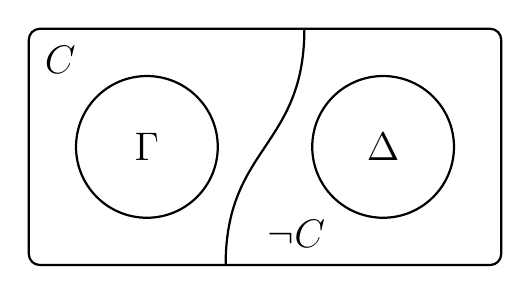
\begin{tikzpicture}[node distance=2cm, auto, thick]
    \draw [rounded corners] (0,0) -- (6,0) -- (6,3) -- (0,3) --  cycle;
    \draw (1.5,1.5) circle (0.9cm);
    \draw (4.5,1.5) circle (0.9cm);
    \path node at (1.5,1.5) {\Large $\Gamma$};
    \path node at (4.5,1.5) {\Large $\Delta$};
    \path node at (0.4,2.6) {\Large $\formula{C}$};
    \path node at (3.4,0.4) {\Large $\lnot \formula{C}$};
    \draw (2.5,0) .. controls (2.5,1.5) and (3.5,1.5) .. (3.5,3);
  \end{tikzpicture}
  \caption{$!C$, $\Gamma$ અને~$\Delta$ને પૃથક કરે છે}
  \ollabel{fig:sep}
\end{figure}


\begin{lem}\ollabel{lem:sep1}
ધારો કે $\Lang{L}_0$ એ એવી ભાષા છે જેમાં $\Gamma$ અને~$\Delta$
\emph{બંને}માં આવતા દરેક અચળ, ફલન અને વિધેય
($\doteq$ સિવાયના) છે, અને $n\ge 0$ માટે અનંત નવા અચળો
$\Obj c_n$ ઉમેરીને $\Lang{L}'_0$ મેળવાય છે. તો જો $\Gamma$ અને
$\Delta$, $\Lang{L}_0$માં અપૃથક્કરણીય હોય, તો તેઓ $\Lang{L}'_0$માં
પણ અપૃથક્કરણીય છે.
\end{lem}

\begin{proof}
આપણે પરોક્ષ રીતે આગળ વધીએ: વિરોધાભાસ માટે ધારો કે $\Gamma$ અને
$\Delta$, $\Lang{L}'_0$માં પૃથક્કરણીય છે. તો કોઈ $!C\in\Lang{L}_0$
માટે $\Gamma \Entails \Subst{!C}{c}{x}$ અને $\Delta \Entails \lnot
\Subst{!C}{c}{x}$ (અહીં $c$ નવો અચળ છે---$!C$માં આવા એકથી
વધુ નવા અચળ હોય તે કિસ્સો સમાન છે). સઘનતાથી, $\Gamma$નો
કોઈ \emph{સાન્ત} ઉપગણ~$\Gamma_0$ અને $\Delta$નો કોઈ \emph{સાન્ત}
ઉપગણ~$\Delta_0$ એવા છે કે $\Gamma_0 \Entails \Subst{!C}{c}{x}$ અને
$\Delta_0 \Entails \lnot \Subst{!C}{c}{x}$. $\Gamma_0$નાં બધાં
સૂત્રોના સંયોજનને~$!G$ અને $\Delta_0$નાં બધાં સૂત્રોના
સંયોજનને~$!H$ કહો. તો
\begin{align*}
  !G & \Entails \Subst{!C}{c}{x}, & !H  \Entails \lnot \Subst{!C}{c}{x}.
\end{align*}
પહેલામાંથી સર્વત્રીકરણ વડે $!G \Entails \lforall[x][!C]$ મળે છે;
બીજામાંથી પ્રતિપક્ષન વડે $\Subst{!C}{c}{x} \Entails \lnot !H$, અને
તેથી $\lforall[x][!C] \Entails \lnot !H$ પણ મળે છે. ફરી પ્રતિપક્ષનથી
$!H \Entails \lnot \lforall[x][!C]$. એકદિશવર્ધિતાથી,
\begin{align*}
  \Gamma &\Entails \lforall[x][!C], &
  \Delta & \Entails \lnot \lforall[x][!C],
\end{align*}
અને તેથી $\lforall[x][!C]$, $\Gamma$ અને~$\Delta$ને $\Lang{L}_0$માં
પૃથક કરે છે.
\sourcecorrection{OLINT-001}{સ્થિર અંગ્રેજી મૂળની
  \texttt{separation.tex}, પંક્તિ~75માં પૂર્વધારણા~$!H$ના સ્થાને
  અગાઉ ક્યાંય વ્યાખ્યાયિત ન થયેલું~$\delta$ આવે છે. પ્રતિપક્ષનથી
  મેળવવાના નિષ્કર્ષમાં અહીં $\lnot !H$ પુનઃસ્થાપિત કર્યું છે.}
\end{proof}

\begin{lem}\ollabel{lem:sep2}
ધારો કે $\Gamma \cup \{ \lexists[x][!S] \}$ અને~$\Delta$
અપૃથક્કરણીય છે, અને $c$ એવો નવો અચળ છે જે $\Gamma$,
$\Delta$ કે~$!S$માં આવતો નથી. તો $\Gamma \cup \{ \lexists[x][!S],
\Subst{!S}{c}{x} \}$ અને~$\Delta$ પણ અપૃથક્કરણીય છે.
\end{lem}

\begin{proof}
વિરોધાભાસ માટે ધારો કે $!C$, $\Gamma \cup \{ \lexists[x][!S],
\Subst{!S}{c}{x}\}$ અને~$\Delta$ને પૃથક કરે છે, જ્યારે $\Gamma \cup
\{\lexists[x][!S] \}$ અને~$\Delta$ અપૃથક્કરણીય છે. આપણે બે કિસ્સા
પાડીએ છીએ:
\sourcecorrection{OLINT-002}{સ્થિર અંગ્રેજી મૂળની
  \texttt{separation.tex}, પંક્તિ~95માં $\lexists$ના સૂત્ર-દલીલખંડને
  જરૂરી ચોરસ કૌંસને બદલે વાંકિયા કૌંસમાં મૂક્યો છે; તેથી તે
  ક્વાન્ટિફાયરના વ્યાપ તરીકે લેવાતો નથી. અહીં
  \texttt{\string\lexists[x][!S]} પુનઃસ્થાપિત કર્યું છે.}
\begin{enumerate}
\item $c$, $!C$માં આવતો નથી: આ કિસ્સામાં $\Gamma \cup
  \{\lexists[x][!S], \lnot!C \}$ સંતોષ્ય છે (નહિતર $!C$, $\Gamma
  \cup \{\lexists[x][!S] \}$ અને~$\Delta$ને પૃથક કરે). તેમાં
  $\Subst{!S}{c}{x}$ ઉમેર્યા પછી પણ તે સંતોષ્ય રહે છે, તેથી અંતે
  $!C$, $\Gamma \cup \{ \lexists[x][!S], \Subst{!S}{c}{x} \}$ અને
  $\Delta$ને પૃથક કરતું નથી.
\item $c$, $!C$માં આવે છે, જેથી $!C$નું સ્વરૂપ
  $\Subst{!C}{c}{x}$ છે. ત્યારે
  \[
  \Gamma \cup \{ \lexists[x][!S], \Subst{!S}{c}{x}\} \Entails \Subst{!C}{c}{x},
  \]
  અને તેથી નિગમન પ્રમેય તથા સર્વત્રીકરણ વડે
  $\Gamma, \lexists[x][!S] \Entails \lforall[x][(!S \lif !C)]$,
  અને છેવટે $\Gamma \cup \{ \lexists[x][!S] \} \Entails
  \lexists[x][!C]$. બીજી તરફ, $\Delta \Entails \lnot
  \Subst{!C}{c}{x}$ અને તેથી સર્વત્રીકરણ વડે $\Delta \Entails \lnot
  \lexists[x][!C]$. એટલે $\Gamma \cup \{\lexists[x][!S] \}$ અને
  $\Delta$ પૃથક્કરણીય છે, જે વિરોધાભાસ છે.
\end{enumerate}
\end{proof}
% END OLP-0200
\endgroup


\begingroup
\makeatletter\def\ol@sectioncs{section}\makeatother

% BEGIN OLP-0201
\olfileid{mod}{int}{prf}

\section{ક્રેગનું અંતર્વેશન પ્રમેય}
\phantomsection\label{guunit:OLP-0201}


\begin{thm}[ક્રેગનું અંતર્વેશન પ્રમેય]
\ollabel{thm:interpol}
જો $\Entails !A \lif !B$, તો એવું વાક્ય~$!C$ છે કે
$\Entails !A \lif !C$ અને $\Entails !C \lif !B$, અને $!C$માં આવતો
દરેક અચળ, ફલન અને વિધેય ($\eq$ સિવાયનો)
$!A$ અને~$!B$ બંનેમાં આવે છે. વાક્ય~$!C$ને $!A$ અને~$!B$નો
\emph{અંતર્વેશક} કહે છે.
\end{thm}

\begin{proof}
ધારો કે $\Lang{L}_1$, $!A$ની ભાષા છે અને $\Lang{L}_2$, $!B$ની ભાષા
છે. $\Lang{L}_0 = \Lang{L}_1 \cap \Lang{L}_2$ રાખો. દરેક $i \in
\{0, 1, 2 \}$ માટે, $\Lang{L}_i$માં અનંત નવા અચળો
$\Obj c_0, \Obj c_1, \Obj c_2, \dots$ ઉમેરીને $\Lang{L}'_i$ મેળવો.

જો $!A$ અસંતોષ્ય હોય, તો $\lexists[x][\eq/[x][x]]$ અંતર્વેશક છે.
જો $\lnot !B$ અસંતોષ્ય હોય (અને તેથી $!B$ પ્રામાણ્ય હોય), તો
$\lexists[x][\eq[x][x]]$ અંતર્વેશક છે. તેથી આપણે $!A$ અને
$\lnot !B$ બંને સંતોષ્ય છે એમ પણ ધારી શકીએ છીએ.

અંતર્વેશન પ્રમેયનું પ્રતિપક્ષી સ્વરૂપ સાબિત કરવા માટે ધારો કે $!A$
અને~$!B$ માટે કોઈ અંતર્વેશક નથી. બીજા શબ્દોમાં, ધારો કે $\{!A\}$ અને
$\{\lnot !B\}$, $\Lang{L}_0$માં અપૃથક્કરણીય છે.

આપણો ઉદ્દેશ જોડ $(\{ !A \}, \{\lnot!B\})$ને કોઈ મહત્તમ
અપૃથક્કરણીય જોડ $(\Gamma^*, \Delta^*)$ સુધી વિસ્તારવાનો છે.
$!A_0$, $!A_1$, $!A_2$,~\dots એ $\Lang{L}'_1$નાં વાક્યોની
ગણના અને $!B_0$, $!B_1$, $!B_2$,~\dots એ $\Lang{L}'_2$નાં
વાક્યોની ગણના હોય. નીચે પ્રમાણે $n\ge0$ માટે વાક્યોના
ગણોની બે વધતી શ્રેણીઓ $(\Gamma_n,\Delta_n)$ વ્યાખ્યાયિત કરીએ. $\Gamma_0
= \{!A\}$ અને $\Delta_0=\{\lnot !B\}$ રાખો. $(\Gamma_n,\Delta_n)$
પહેલેથી વ્યાખ્યાયિત છે એમ ધારીને, $\Gamma_{n+1}$ અને
$\Delta_{n+1}$ને આ પ્રમાણે વ્યાખ્યાયિત કરો:
\sourcecorrection{OLINT-003}{સ્થિર અંગ્રેજી મૂળની
  \texttt{interpolation-proof.tex}, પંક્તિઓ~41--43માં $!A_n$ અને
  $!B_n$ને અનુક્રમે $\Lang{L}_1$ અને $\Lang{L}_2$નાં વાક્યોની ગણના
  કહેવાય છે. પરંતુ પછીની પંક્તિઓ~107--108માં રચાયેલા ગણો
  $\Lang{L}'_1$ અને $\Lang{L}'_2$માં પૂર્ણ સુસંગત હોવાનો દાવો થાય છે,
  જેના માટે નવા અચળો ધરાવતાં વાક્યોની પણ ગણના જરૂરી છે. અહીં બંને
  વિસ્તૃત ભાષાઓ પર ગણના પુનઃસ્થાપિત કરી છે.}
\begin{enumerate}
\item જો $\Gamma_n \cup \{!A_n \}$ અને~$\Delta_n$, $\Lang{L}'_0$માં
  અપૃથક્કરણીય હોય, તો $!A_n$ને $\Gamma_{n+1}$માં મૂકો. વધુમાં, જો
  $!A_n$ કોઈ અસ્તિત્વવાચક સૂત્ર~$\lexists[x][!S]$ હોય, તો
  $\Gamma_n$, $\Delta_n$, $!A_n$ કે~$!B_n$માં ન આવતો નવો
  અચળ~$c$ પસંદ કરીને $\Subst{!S}{c}{x}$ને
  $\Gamma_{n+1}$માં મૂકો.
\item જો $\Gamma_{n+1}$ અને $\Delta_n \cup \{!B_n \}$,
  $\Lang{L}'_0$માં અપૃથક્કરણીય હોય, તો $!B_n$ને $\Delta_{n+1}$માં
  મૂકો. વધુમાં, જો $!B_n$ કોઈ અસ્તિત્વવાચક
  સૂત્ર~$\lexists[x][!S]$ હોય, તો $\Gamma_{n+1}$, $\Delta_n$,
  $!A_n$ કે~$!B_n$માં ન આવતો નવો અચળ~$c$ પસંદ કરીને
  $\Subst{!S}{c}{x}$ને $\Delta_{n+1}$માં મૂકો.
\end{enumerate}
છેવટે, આ પ્રમાણે વ્યાખ્યા કરો:
\begin{align*}
  \Gamma^* & = \bigcup_{n\ge 0} \Gamma_n, &
  \Delta^* & = \bigcup_{n\ge 0} \Delta_n.
\end{align*}
હવે $n$ પરના સમકાલીન આગમનથી આપણે નીચેના દાવા સાબિત કરી શકીએ છીએ:
\begin{enumerate}
\item\ollabel{part-a} $\Gamma_n$ અને~$\Delta_n$, $\Lang{L}'_0$માં
  અપૃથક્કરણીય છે;
\item\ollabel{part-b} $\Gamma_{n+1}$ અને~$\Delta_n$,
  $\Lang{L}'_0$માં અપૃથક્કરણીય છે.
\end{enumerate}
\olref{part-a}નો આધાર \olref[sep]{lem:sep1} આપે છે. ભાગ
\olref{part-b} માટે આપણે ત્રણ કિસ્સા પાડવા પડે છે:
\begin{enumerate}
\item જો $\Gamma_0 \cup \{!A_0 \}$ અને~$\Delta_0$ પૃથક્કરણીય હોય,
  તો $\Gamma_1=\Gamma_0$ અને \olref{part-b}, \olref{part-a} જ છે;
\item જો $\Gamma_1 = \Gamma_0 \cup\{!A_0\}$, તો રચના મુજબ
  $\Gamma_1$ અને~$\Delta_0$ અપૃથક્કરણીય છે.
\item હવે માત્ર $!A_0$ અસ્તિત્વવાચક હોય તે કિસ્સો બાકી રહે છે, જેમાં
  $\Gamma_1 = \Gamma_0 \cup \{ \lexists[x][!S], \Subst{!S}{c}{x}
  \}$. રચના મુજબ $\Gamma_0 \cup \{ \lexists[x][!S]\}$ અને
  $\Delta_0$ અપૃથક્કરણીય છે, તેથી \olref[sep]{lem:sep2} મુજબ
  $\Gamma_0 \cup \{ \lexists[x][!S], \Subst{!S}{c}{x} \}$ અને
  $\Delta_0$ પણ અપૃથક્કરણીય છે.
\end{enumerate}
આથી ઉપરના \olref{part-a} અને \olref{part-b} માટે આગમનનો આધાર પૂરો
થાય છે. હવે આગમન-પગલું લઈએ. \olref{part-a} માટે, જો $!B_n$ને
$\Delta_{n+1}$માં મૂકવામાં આવે, તો રચના મુજબ $\Gamma_{n+1}$ અને
$\Delta_n\cup\{!B_n\}$ અપૃથક્કરણીય છે; અને જો $!B_n$ અસ્તિત્વવાચક
હોય, તો સાક્ષી ઉમેર્યા પછીનો $\Delta_{n+1}$ પણ
\olref[sep]{lem:sep2} મુજબ અપૃથક્કરણીય રહે છે. જો
$\Delta_{n+1}=\Delta_n$ (કારણ કે $\Gamma_{n+1}$ અને
$\Delta_n\cup\{!B_n\}$ પૃથક્કરણીય છે), તો \olref{part-b} માટેની
આગમન-પરિકલ્પના વાપરીએ. \olref{part-b}ના આગમન-પગલા માટે, જો
$!A_{n+1}$ને $\Gamma_{n+2}$માં મૂકવામાં આવે, તો રચના મુજબ
$\Gamma_{n+1}\cup\{!A_{n+1}\}$ અને~$\Delta_{n+1}$ અપૃથક્કરણીય છે;
અને જો $!A_{n+1}$ અસ્તિત્વવાચક હોય, તો સાક્ષી ઉમેર્યા પછીનો
$\Gamma_{n+2}$ પણ \olref[sep]{lem:sep2} મુજબ અપૃથક્કરણીય રહે છે. જો
$\Gamma_{n+2}=\Gamma_{n+1}$, તો હમણાં જ સાબિત કરેલો
\olref{part-a}નો આગમન-કિસ્સો વાપરીએ. આથી \olref{part-a} અને
\olref{part-b} પરનું આગમન પૂરું થાય છે.
\sourcecorrection{OLINT-004}{સ્થિર અંગ્રેજી મૂળની
  \texttt{interpolation-proof.tex}, પંક્તિઓ~88--96માં અસ્તિત્વવાચક
  $!B_n$ કે $!A_{n+1}$ સ્વીકારાય ત્યારે સાક્ષી-સૂત્ર પણ ઉમેરવાની
  અગાઉની સૂચના હોવા છતાં અનુક્રમે
  $\Delta_{n+1}=\Delta_n\cup\{!B_n\}$ અને
  $\Gamma_{n+2}=\Gamma_{n+1}\cup\{!A_{n+1}\}$ લખાયું છે. અહીં
  સ્વીકારેલો વિધાન અને પછી ઉમેરાતો સાક્ષી અલગ કરીને, લેમા
  \olref[sep]{lem:sep2}નો ઉપયોગ બંને પૂર્ણ ગણો પર સ્પષ્ટ કર્યો છે.}

આમાંથી ફલિત થાય છે કે $\Gamma^*$ અને~$\Delta^*$ અપૃથક્કરણીય છે;
નહિતર સઘનતાથી એવું $n\ge0$ અને એવું $\Lang{L}'_0$-વિધાન મળે જે
$\Gamma_n$ અને~$\Delta_n$ને પૃથક કરે, જે \olref{part-a}ની વિરુદ્ધ
છે. ખાસ કરીને, $\Gamma^*$ અને~$\Delta^*$ સુસંગત છે: કારણ કે પહેલો
અથવા બીજો અસુસંગત હોય, તો અનુક્રમે $\lexists[x][\eq/[x][x]]$ અથવા
$\lforall[x][\eq[x][x]]$ તેમને પૃથક કરે.
\sourcecorrection{OLINT-005}{સ્થિર અંગ્રેજી મૂળની
  \texttt{interpolation-proof.tex}, પંક્તિઓ~100--102માં કોઈ
  $n\ge0$ પોતે $\Gamma_n$ અને $\Delta_n$ને પૃથક કરે છે તેમ લખાયું
  છે. પૃથક્કર્તા વિધાન હોય છે; સઘનતા માત્ર એવું એક જ~$n$ આપે છે જેમાં
  તેના માટે જરૂરી બંને સાન્ત ઉપગણો આવી જાય. અહીં એ વિધાન અને~$n$ની
  જુદી ભૂમિકાઓ સ્પષ્ટ કરી છે.}

હવે આપણે બતાવીએ કે $\Gamma^*$, $\Lang{L}'_1$માં પૂર્ણ સુસંગત છે અને
એ જ રીતે $\Delta^*$, $\Lang{L}'_2$માં પૂર્ણ સુસંગત છે. પહેલા માટે,
ધારો કે કોઈ $n\ge0$ માટે $!A_n\notin\Gamma^*$ અને $\lnot !A_n
\notin\Gamma^*$. જો $!A_n\notin\Gamma^*$, તો $\Gamma_n\cup\{!A_n\}$
$\Delta_n$થી પૃથક્કરણીય છે, તેથી એવું $!C\in\Lang{L}'_0$ છે કે આ
બંને વાતો સાચી છે:
\begin{align*}
  \Gamma^* & \Entails !A_n \lif !C, &
  \Delta^* & \Entails \lnot !C.
\end{align*}
એ જ રીતે, જો $\lnot !A_n\notin\Gamma^*$, તો એવું $!C'\in
\Lang{L}'_0$ છે કે આ બંને વાતો સાચી છે:
\begin{align*}
  \Gamma^* & \Entails \lnot !A_n \lif !C', &
  \Delta^* & \Entails \lnot !C'.
\end{align*}
વિધાનાત્મક તર્કશાસ્ત્રથી $\Gamma^*\Entails !C\lor !C'$ અને
$\Delta^*\Entails\lnot(!C\lor !C')$, તેથી $!C\lor !C'$,
$\Gamma^*$ અને~$\Delta^*$ને પૃથક કરે છે. સમાન દલીલથી $\Delta^*$ પૂર્ણ
છે.

છેવટે, આપણે બતાવીએ કે $\Gamma^*\cap\Delta^*$, $\Lang{L}'_0$માં પૂર્ણ
સુસંગત છે. તે સુસંગત ગણોનો છેદ હોવાથી દેખીતી રીતે સુસંગત છે. પૂર્ણતા
બતાવવા $!S\in\Lang{L}'_0$ લો. હવે $\Gamma^*$, $\Lang{L'_1}
\supseteq\Lang{L'_0}$માં પૂર્ણ છે અને એ જ રીતે $\Delta^*$,
$\Lang{L'_2}\supseteq\Lang{L'_0}$માં પૂર્ણ છે. તેથી કાં તો
$!S\in\Gamma^*$ અથવા $\lnot !S\in\Gamma^*$, અને કાં તો
$!S\in\Delta^*$ અથવા $\lnot !S\in\Delta^*$. જો $!S\in\Gamma^*$ અને
$\lnot !S\in\Delta^*$, તો $!S$, $\Gamma^*$ અને~$\Delta^*$ને પૃથક
કરે; અને જો $\lnot !S\in\Gamma^*$ અને $!S\in\Delta^*$, તો
$\Gamma^*$ અને~$\Delta^*$ને $\lnot !S$ પૃથક કરે. આથી, કાં તો
$!S\in\Gamma^*\cap\Delta^*$
અથવા $\lnot !S\in\Gamma^*\cap\Delta^*$, અને
$\Gamma^*\cap\Delta^*$ પૂર્ણ છે.

$\Gamma^*$ પૂર્ણ સુસંગત હોવાથી તેને એવો નિદર્શ $\Struct{M}'_1$ મળે
છે જેનું પ્રદેશ~$\Domain{M'_1}$, અચળોનાં અર્થઘટનો
$\Assign{c}{M'_1}$ એવા અને માત્ર એવા ઘટકોનું બનેલું છે---પૂર્ણતા
પ્રમેયની સાબિતીની જેમ (\olref[fol][com][cth]{thm:completeness}). એ જ
રીતે, $\Delta^*$ને એવો નિદર્શ~$\Struct{M}'_2$ મળે છે જેનું
પ્રદેશ~$\Domain{M'_2}$, અચળોનાં અર્થઘટનો
$\Assign{c}{M'_2}$થી બનેલું છે.

$\Struct{M'_1}$માંથી $\Lang{L'_1}\setminus\Lang{L'_0}$માંના
અચળો, ફલનો અને વિધેયોનાં અર્થઘટનો કાઢીને
$\Struct{M_1}$ મેળવો, અને $\Struct{M_2}$ પણ એ જ રીતે મેળવો. ત્યારે
$h(\Assign{c}{M'_1})=\Assign{c}{M'_2}$થી વ્યાખ્યાયિત કરેલો નકશો
$h\colon M_1\to M_2$, $\Lang{L}'_0$માં એકરૂપતા છે, કારણ કે બતાવ્યા
પ્રમાણે $\Gamma^*\cap\Delta^*$, $\Lang{L}'_0$માં પૂર્ણ સુસંગત છે.
આનું કારણ એ છે કે કોઈ પણ $\Lang{L}'_0$-વાક્ય કાં તો $\Gamma^*$
અને~$\Delta^*$ બંનેમાં આવે છે અથવા એકેયમાં આવતું નથી: તેથી
$\Assign{c}{M'_1}\in\Assign{P}{M'_1}$ જો અને માત્ર જો
$\Atom{P}{c}\in\Gamma^*$, જો અને માત્ર જો $\Atom{P}{c}\in\Delta^*$,
જો અને માત્ર જો $\Assign{c}{M'_2}\in\Assign{P}{M'_2}$. એકરૂપતાની
બીજી શરતો પણ એ જ રીતે સ્થાપિત કરી શકાય છે.

હવે ભાષા~$\Lang{L_1}\cup\Lang{L_2}$ માટેનો નિદર્શ
$\Struct{M}$ આ પ્રમાણે વ્યાખ્યાયિત કરીએ:
\begin{enumerate}
\item પ્રદેશ~$\Domain{M}$ એ $\Domain{M_2}$ જ છે, એટલે બધા
  ઘટકો~$\Assign{c}{M'_2}$નો ગણ;
\item જો કોઈ વિધેય~$P$, $\Lang{L_2}\setminus\Lang{L_1}$માં
  હોય, તો $\Assign{P}{M}=\Assign{P}{M'_2}$;
\item જો કોઈ વિધેય-સંકેત~$P$, $\Lang{L}_1\setminus\Lang{L}_2$માં હોય, તો
  $\Assign{P}{M}=h(\Assign{P}{M'_1})$, એટલે
  $\tuple{\Assign{c_1}{M'_2},\dots,\Assign{c_n}{M'_2}}\in
  \Assign{P}{M}$ જો અને માત્ર જો
  $\tuple{\Assign{c_1}{M'_1},\dots,\Assign{c_n}{M'_1}}\in
  \Assign{P}{M'_1}$.
\item જો કોઈ વિધેય~$P$, $\Lang{L}_0$માં હોય, તો
  $\Assign{P}{M}=\Assign{P}{M'_2}=h(\Assign{P}{M'_1})$.
\item ફલનોને, જેમાં અચળો પણ સામેલ છે,
  $\Lang{L}_1\cup\Lang{L}_2$ પર એ જ રીતે સંભાળો.
\end{enumerate}
\sourcecorrection{OLINT-006}{સ્થિર અંગ્રેજી મૂળની
  \texttt{interpolation-proof.tex}, પંક્તિ~173માં
  $P\in\Lang{L}_1\setminus\Lang{L}_2$ હોવા છતાં તેના અર્થઘટનને
  $\Struct{M'_2}$માંથી લઈ $h$ લગાડવામાં આવ્યું છે. $\Struct{M'_2}$
  પાસે $P$નું અર્થઘટન હોવું જરૂરી નથી અને $h$નું ક્ષેત્ર પણ
  $M_1$ છે. તરત પછી આપેલી ``એટલે'' શરત મુજબ અહીં
  $h(\Assign{P}{M'_1})$ પુનઃસ્થાપિત કર્યું છે.}

છેવટે, સૂત્રો પરના આગમનથી બતાવી શકાય છે કે $\Lang{L}_1$નાં
બધાં સૂત્રો માટે $\Struct{M'_1}$ના $\Lang{L}_1$-ન્યૂનરૂપમાં
સંતોષ, $h$ મારફતે $\Struct{M}$ના $\Lang{L}_1$-ન્યૂનરૂપમાં સંતોષને
બરાબર અનુરૂપ છે, અને $\Lang{L}_2$નાં બધાં સૂત્રો માટે
$\Struct{M}$ તથા $\Struct{M'_2}$નાં $\Lang{L}_2$-ન્યૂનરૂપોમાં સંતોષ
સંમત થાય છે. ખાસ કરીને,
$\Struct{M'_1}\Entails\Gamma^*$ તથા $!A\in\Gamma^*$, અને
$\Struct{M'_2}\Entails\Delta^*$ તથા $\lnot !B\in\Delta^*$ હોવાથી
$\Struct{M}\Entails !A$ અને $\Struct{M}\Entails\lnot !B$. તેથી
$\not\Entails !A\lif !B$. આથી ક્રેગના અંતર્વેશન પ્રમેયની સાબિતી
પૂરી થાય છે.
\sourcecorrection{OLINT-007}{સ્થિર અંગ્રેજી મૂળની
  \texttt{interpolation-proof.tex}, પંક્તિઓ~183--187માં
  $\Struct{M}$ને માત્ર $\Lang{L}_1\cup\Lang{L}_2$ માટે વ્યાખ્યાયિત
  કર્યા પછી તે નવા અચળો ધરાવતી વિસ્તૃત ભાષાઓ $\Lang{L}'_1$ અને
  $\Lang{L}'_2$નાં બધાં સૂત્રો પર સંમત થાય છે અને
  $\Gamma^*\cup\Delta^*$ને સંતોષે છે એવો અપરિભાષિત દાવો થાય છે.
  અહીં જરૂરી અને પર્યાપ્ત ન્યૂનરૂપ-દાવો મૂક્યો છે: $h$ પહેલા નિદર્શના
  $\Lang{L}_1$-ભાગને પરિવહિત કરે છે અને બીજાનો
  $\Lang{L}_2$-ભાગ યથાવત્ રહે છે; તેથી મૂળ વાક્યો $!A$ અને
  $\lnot !B$ સાચાં રહે છે.}
\end{proof}
% END OLP-0201
\endgroup


\begingroup
\makeatletter\def\ol@sectioncs{section}\makeatother

% BEGIN OLP-0202
\olfileid{mod}{int}{def}

\section{વ્યાખ્યેયતા પ્રમેય}
\phantomsection\label{guunit:OLP-0202}


અંતર્વેશન પ્રમેયનો એક મહત્વનો ઉપયોગ બેથનું વ્યાખ્યેયતા પ્રમેય છે.
$n$-સ્થાની સંબંધ~$R$ને વ્યાખ્યાયિત કરવા માટે આપણે $R$ ન આવતો હોય
અને $n$ મુક્ત ચલો ધરાવતો કોઈ સૂત્ર~$!C$ આપી શકીએ
છીએ. આ $!C$ દ્વારા $R$ની \emph{સ્પષ્ટ} વ્યાખ્યા થાય. પછી આપણે એમ
પણ કહી શકીએ કે $n$-સ્થાની વિધેય~$P$ ધરાવતી કોઈ ભાષામાં
સિદ્ધાંત~$\Sigma(P)$, $P$ને સ્પષ્ટ રીતે વ્યાખ્યાયિત કરે છે જો તેમાં
ઔપચારિક કરેલી સ્પષ્ટ વ્યાખ્યા હોય (અથવા ઓછામાં ઓછું તેમાંથી ફલિત થતી
હોય), એટલે કે,
\[
\Sigma(P) \Entails \lforall[x_1][\dots
  \lforall[x_n][(\Atom{P}{x_1,\dots, x_n} \liff !C(x_1, \dots,
    x_n))]].
\]
પરંતુ સંબંધને વ્યાખ્યાયિત કરવાનો---તેને સંપૂર્ણપણે નિશ્ચિત કરવાના
અર્થમાં---સ્પષ્ટ વ્યાખ્યા માત્ર એક માર્ગ છે. સિદ્ધાંત એવો પણ હોઈ શકે
કે કોઈ પણ નિદર્શમાં ભાષાના બાકીના ભાગના અર્થઘટનથી $P$નું
અર્થઘટન નિશ્ચિત થાય. વ્યાખ્યેયતા પ્રમેય કહે છે કે જ્યારે પણ સિદ્ધાંત
$P$નું અર્થઘટન આ રીતે નિશ્ચિત કરે---જ્યારે તે $P$ને \emph{ગૂઢ રીતે
વ્યાખ્યાયિત કરે}---ત્યારે તે તેને સ્પષ્ટ રીતે પણ વ્યાખ્યાયિત કરે છે.

\begin{defn}
ધારો કે $\Lang{L}$ એવી ભાષા છે જેમાં વિધેય~$P$ નથી.
$\Lang{L}\cup\{P\}$નાં વાક્યોનો ગણ~$\Sigma(P)$, $P$ને ત્યારે
અને માત્ર ત્યારે \emph{સ્પષ્ટ રીતે વ્યાખ્યાયિત કરે છે} જ્યારે
$\Lang{L}$નું એવું સૂત્ર~$!C(x_1,\dots,x_n)$ છે કે
\[
\Sigma(P) \Entails \lforall[x_1][\dots
  \lforall[x_n][(\Atom{P}{x_1,\dots, x_n} \liff !C(x_1, \dots,
    x_n))]].
\]
\end{defn}

\begin{defn}
ધારો કે $\Lang{L}$ એવી ભાષા છે જેમાં વિધેયો $P$
અને~$P'$ નથી. $\Lang{L}\cup\{P\}$નાં વાક્યોનો ગણ~$\Sigma(P)$,
$P$ને ત્યારે અને માત્ર ત્યારે \emph{ગૂઢ રીતે વ્યાખ્યાયિત કરે છે}
જ્યારે
\[
\Sigma(P) \cup \Sigma(P') \Entails \lforall[x_1][\dots
  \lforall[x_n][(\Atom{P}{x_1,\dots, x_n} \liff \Atom{P'}{x_1,\dots,
      x_n})]],
\]
જ્યાં $\Sigma(P')$ એ $\Sigma(P)$માં $P$ને સર્વત્ર $P'$થી બદલીને
મળતું પરિણામ છે.
\end{defn}

બીજા શબ્દોમાં, કોઈ પણ નિદર્શ~$\Struct{M}$ અને $R,R'\subseteq
\Domain{M}^n$ માટે, જો $\Expan{M}{R}\Entails\Sigma(P)$ અને
$\Expan{M}{R'}\Entails\Sigma(P')$ બંને, તો $R=R'$; અહીં
$\Expan{M}{R}$ એ $\Lang{L}$ના $\Lang{L}\cup\{P\}$ સુધીના વિસ્તાર
માટેની એવી સંરચના~$\Struct{M'}$ છે કે $\Assign{P}{M'}=R$, અને
$\Expan{M}{R'}$ માટે પણ એ જ રીતે.

\begin{thm}[બેથનું વ્યાખ્યેયતા પ્રમેય]
$\Lang{L}\cup\{P\}$નાં વાક્યોનો ગણ~$\Sigma(P)$, $P$ને ગૂઢ
રીતે વ્યાખ્યાયિત કરે છે જો અને માત્ર જો $\Sigma(P)$, $P$ને સ્પષ્ટ
રીતે વ્યાખ્યાયિત કરે છે.
\end{thm}
\sourcecorrection{OLINT-008}{સ્થિર અંગ્રેજી મૂળની
  \texttt{definability.tex}, પંક્તિઓ~66--68માં પ્રમેય $\Sigma(P)$ને
  સૂત્રોનો ગણ કહે છે, જ્યારે તરત અગાઉની બંને વ્યાખ્યાઓ તેને
  વાક્યોનો ગણ કહે છે અને નીચેની સાબિતી પણ સાન્ત ઉપગણનાં
  વાક્યોના સંયોજન પર ચાલે છે. અહીં વ્યાખ્યાઓ અને સાબિતી મુજબ
  વાક્યો પુનઃસ્થાપિત કર્યાં છે.}
\sourcecorrection{OLINT-009}{એ જ મૂળની પંક્તિ~67માં દ્વિમુખી શરતના
  ``if and only if''માંથી છેલ્લું ``if'' છૂટી ગયું છે. અહીં સંપૂર્ણ
  દ્વિમુખી શરત પુનઃસ્થાપિત કરી છે.}

\begin{proof}
જો $\Sigma(P)$, $P$ને સ્પષ્ટ રીતે વ્યાખ્યાયિત કરે, તો આ બંને સાચાં
છે:
\begin{align*}
  \Sigma(P) & \Entails & \lforall[x_1][\dots \lforall[x_n]
    [(\Atom{P}{x_1,\dots, x_n} \liff !C(x_1,\dots,x_n))]]\\
  \Sigma(P') & \Entails & \lforall[x_1][\dots \lforall[x_n]
    [(\Atom{P'}{x_1,\dots, x_n} \liff !C(x_1,\dots,x_n))]]
\end{align*}
અને નિષ્કર્ષ ફલિત થાય છે. વ્યસ્ત દિશા માટે ધારો કે $\Sigma(P)$,
$P$ને ગૂઢ રીતે વ્યાખ્યાયિત કરે છે. પહેલા $\Lang{L}$માં અચળો
$c_1$,~\dots,~$c_n$ ઉમેરીએ. ત્યારે
\[
\Sigma(P) \cup \Sigma(P') \Entails
\Atom{P}{c_1, \dots, c_n} \to \Atom{P'}{c_1, \dots, c_n}.
\]
સઘનતાથી એવા સાન્ત ગણો $\Delta_0\subseteq\Sigma(P)$ અને
$\Delta_1\subseteq\Sigma(P')$ છે કે
\[
\Delta_0 \cup \Delta_1 \Entails
\Atom{P}{c_1, \dots, c_n} \to \Atom{P'}{c_1, \dots, c_n}.
\]
એવા બધા વાક્યો~$!A(P)$નું સંયોજન~$!D(P)$ કહો કે કાં તો
$!A(P)\in\Delta_0$ અથવા $!A(P')\in\Delta_1$, અને એવા બધા
વાક્યો~$!A(P')$નું સંયોજન~$!D(P')$ કહો કે કાં તો
$!A(P)\in\Delta_0$ અથવા $!A(P')\in\Delta_1$. ત્યારે
$!D(P)\land !D(P')\Entails\Atom{P}{c_1,\dots,c_n}\to
\Atom{P'}{c_1,\dots,c_n}$. આને એવી રીતે ફરી ગોઠવી શકાય કે દરેક
વિધેય, $\Entails$ની એક બાજુ જ આવે:
\sourcecorrection{OLINT-010}{સ્થિર અંગ્રેજી મૂળની
  \texttt{definability.tex}, પંક્તિ~96માં જમણી બાજુનું પરમાણુક સૂત્ર
  આસપાસનાં બધાં દાખલાથી જુદું $P'c_1\dots c_n$ લખાયું છે. અહીં એ જ
  $n$-સ્થાની પરમાણુક સૂત્ર માટેનું આવૃત્તિ-સુસંગત
  \texttt{\string\Atom\{P'\}\{c\_1,\string\dots,c\_n\}} સ્વરૂપ વાપર્યું
  છે.}
\[
!D(P) \land \Atom{P}{c_1, \dots, c_n} \Entails
!D(P') \to \Atom{P'}{c_1, \dots, c_n}.
\]
ક્રેગના અંતર્વેશન પ્રમેય મુજબ $P$ કે~$P'$ ન ધરાવતું એવું
વાક્ય~$!C(c_1,\dots,c_n)$ છે કે
\begin{align*}
  !D(P) \land \Atom{P}{c_1, \dots, c_n} & \Entails !C(c_1,\dots, c_n); \\
  !C(c_1,\dots, c_n) & \Entails !D(P') \to \Atom{P'}{c_1, \dots, c_n}.
\end{align*}
આ બે ફલિતતાઓમાંથી પહેલામાંથી મળે છે: $!D(P)\Entails
\Atom{P}{c_1,\dots,c_n}\lif !C(c_1,\dots,c_n)$. અને બીજામાંથી,
કારણ કે કોઈ $\Lang{L}\cup\{P\}$-નિદર્શ $\Expan{M}{R}\Entails
!A(P)$ જો અને માત્ર જો તેને અનુરૂપ $\Lang{L}\cup\{P'\}$-નિદર્શ
$\Expan{M}{R}\models !A(P')$, આપણને
$!C(c_1,\dots,c_n)\Entails !D(P)\lif\Atom{P}{c_1,\dots,c_n}$ મળે છે,
અને તેમાંથી
\[
!D(P) \Entails !C(c_1,\dots,c_n) \to \Atom{P}{c_1,\dots, c_n}.
\]
બંનેને સાથે મૂકતાં $!D(P)\Entails\Atom{P}{c_1,\dots,c_n}\liff
!C(c_1,\dots,c_n)$ મળે છે, અને એકદિશવર્ધિતા તથા સર્વત્રીકરણથી આ પણ
મળે છે:
\[
\Sigma(P) \Entails
\lforall[x_1][\dots\lforall[x_n][(\Atom{P}{x_1,\dots, x_n} \liff
    !C(x_1,\dots, x_n))]].
\]
\end{proof}
% END OLP-0202
\endgroup


\OLEndChapterHook
% END OLP-0198
\endgroup


\begingroup
\makeatletter\def\ol@sectioncs{section}\makeatother

% BEGIN OLP-0203
\olchapter{mod}{lin}{લિન્ડસ્ટ્રોમનું પ્રમેય}
\olchapterid{mod}{lin}
\phantomsection\label{guunit:OLP-0203}


\begingroup
\makeatletter\def\ol@sectioncs{section}\makeatother

% BEGIN OLP-0204
\olfileid{mod}{lin}{int}
\section{પરિચય}
\phantomsection\label{guunit:OLP-0204}


આ પ્રકરણમાં આપણે પ્રથમ-ક્રમ તર્કશાસ્ત્રનું લિન્ડસ્ટ્રોમ-લક્ષણન સાબિત
કરવાનું લક્ષ્ય રાખીએ છીએ: અમુક વધારાની મર્યાદાઓ હેઠળ સઘનતા અને અધોગામી
લેવેનહાઇમ--સ્કોલેમ પ્રમેયો જે મહત્તમ તર્કશાસ્ત્ર માટે સત્ય છે તે
પ્રથમ-ક્રમ તર્કશાસ્ત્ર છે
(\olref[fol][com][com]{thm:compactness} અને
\olref[fol][com][dls]{thm:downward-ls}). પહેલાં આપણે આ પ્રમેય જેમને લાગુ
પડે છે તે તર્કશાસ્ત્રોના સામાન્ય વર્ગનું વધુ વ્યાપક લક્ષણન જોઈએ. આપણે
પોતાને \emph{સંબંધાત્મક} ભાષાઓ પૂરતા મર્યાદિત રાખીશું, એટલે કે એવી
ભાષાઓ જેમાં માત્ર વિધેયો અને વ્યક્તિ-અચળો હોય, પણ કોઈ
ફલનો ન હોય.
% END OLP-0204
\endgroup


\begingroup
\makeatletter\def\ol@sectioncs{section}\makeatother

% BEGIN OLP-0205
\olfileid{mod}{lin}{alg}
\olsection{અમૂર્ત તર્કશાસ્ત્રો}
\phantomsection\label{guunit:OLP-0205}


\begin{defn}
  \emph{અમૂર્ત તર્કશાસ્ત્ર} એ યુગ્મ $\tuple{L, \models_L}$ છે, જ્યાં
  $L$ એવું વિધેય છે જે દરેક ભાષા~$\Lang{L}$ને
  વાક્યોનો ગણ $L(\Lang{L})$ નિયુક્ત કરે છે, અને $\models_L$ એ
  ભાષા~$\Lang{L}$ માટેની સંરચનાઓ તથા $L(\Lang{L})$ના
  ઘટકો વચ્ચેનો સંબંધ છે. ખાસ કરીને, $\tuple{F, \models}$ એ
  સામાન્ય પ્રથમ-ક્રમ તર્કશાસ્ત્ર છે; એટલે કે, $F$ એવું વિધેય છે જે
  ભાષા~$\Lang{L}$ને $\Lang{L}$ના સંકેતોમાંથી બનેલાં પ્રથમ-ક્રમ
  વાક્યોનો ગણ નિયુક્ત કરે છે, અને $\models$ એ પ્રથમ-ક્રમ
  તર્કશાસ્ત્રનો સંતોષ-સંબંધ છે.
  \sourcecorrection{OLLIN-001}{સ્થિર અંગ્રેજી મૂળની
    \texttt{abstract-logics.tex}, પંક્તિઓ~18--20માં પ્રથમ-ક્રમનાં વાક્યો
    ભાષાના માત્ર અચળોમાંથી બને છે એમ કહેવાયું છે, જેથી વિધેય-સંકેતો
    છૂટી જાય છે. $F(\Lang L)$માં ભાષાના બધા સંકેતો વડે બનેલાં
    પ્રથમ-ક્રમ વાક્યો આવે છે; અહીં એ વ્યાપ રાખ્યો છે.}
\end{defn}

નોંધો કે આપેલી ભાષા માટે આપણે હજી પણ પ્રથમ-ક્રમ તર્કશાસ્ત્રમાં
હોય એ જ સંરચનાની વિભાવના વાપરીએ છીએ. પરંતુ આપણે એવું પૂર્વધારતા
નથી કે વાક્યો સામાન્ય રીતે $\Lang{L}$ના મૂળભૂત સંકેતોમાંથી
બનાવાય છે, કે $\models_L$ સંબંધ પણ પ્રથમ-ક્રમ તર્કશાસ્ત્રની જેમ જ
આવર્ત રીતે વ્યાખ્યાયિત થાય છે. તેથી, દાખલા તરીકે, આ તદ્દન સામાન્ય
વ્યાખ્યાનો આશય એવા કિસ્સાઓને પણ આવરી લેવાનો છે જેમાં
$\tuple{L,\models_L}$નાં વાક્યો અનંત લાંબાં સંયોજનો કે વિયોજનો,
$\lexists$ અને $\lforall$ સિવાયના પરિમાણકો (જેમ કે ``એવા અનંત ઘણા
$x$ છે કે \dots''), અથવા કદાચ અનંત લાંબા પરિમાણક-ઉપસર્ગો ધરાવે.
$L(\Lang{L})$નાં ``વાક્યો'' પ્રથમ-ક્રમ તર્કશાસ્ત્રનાં સામાન્ય
વાક્યો હોવાં જરૂરી નથી એ પર ભાર મૂકવા આ પ્રકરણમાં તેમના માટે
ચલો $!E$, $!F$,~\dots વાપરીએ છીએ અને સામાન્ય પ્રથમ-ક્રમ
સૂત્રો માટે $!A$, $!B$,~\dots અનામત રાખીએ છીએ.

\begin{defn}
  વર્ગ $\Setabs{\Struct{M}}{\Struct{M} \models_L !E}$ને
  $\Mod(L){!E}$થી દર્શાવીએ. ભાષા સ્પષ્ટ કરવી જરૂરી હોય તો
  $\Mod[L](L){!E}$ લખીએ. $\Lang{L}$ માટેની બે સંરચનાઓ
  $\Struct{M}$ અને $\Struct{N}$માં $L(\Lang{L})$નાં એ જ
  વાક્યો સાચાં હોય તો તેમને $\tuple{L, \models_L}$માં
  \emph{પ્રાથમિક રીતે સમકક્ષ} કહીએ છીએ અને $\Struct{M}
  \elemequiv[L] \Struct{N}$ લખીએ છીએ.
\end{defn}

\begin{defn}
  ભાષા~$\Lang{L}$ માટેનું અમૂર્ત તર્કશાસ્ત્ર
  $\tuple{L,\models_L}$
  નીચેના ગુણધર્મો સંતોષે તો તેને \emph{સામાન્ય} કહીએ છીએ:
\begin{enumerate}
\item (\emph{$L$-એકદિશવર્ધિતા}) ભાષાઓ $\Lang{L}$ અને
  $\Lang{L'}$ માટે જો $\Lang{L} \subseteq \Lang{L'}$, તો
  $L(\Lang{L}) \subseteq L(\Lang{L'})$.
\item (\emph{વિસ્તાર ગુણધર્મ}) દરેક $!E \in L(\Lang{L})$ માટે
  $\Lang{L}$નો એવો \emph{સાન્ત} ઉપગણ $\Lang{L'}$ છે કે
  $\Struct{M} \models_L !E$ સંબંધ $\Struct{M}$ના $\Lang{L'}$ પરના
  ન્યૂનરૂપ પર જ આધાર રાખે; એટલે કે, $\Struct{M}$ અને $\Struct{N}$નાં
  $\Lang{L'}$ પરનાં ન્યૂનરૂપો સરખાં હોય, તો $\Struct{M} \models_L !E$
  ત્યારે અને માત્ર ત્યારે જ્યારે $\Struct{N} \models_L !E$.
\item (\emph{એકરૂપતા ગુણધર્મ}) જો $\Struct{M} \models_L !E$ અને
  $\Struct{M} \simeq \Struct{N}$, તો $\Struct{N} \models_L !E$ પણ.
\item (\emph{પુનઃનામકરણ ગુણધર્મ}) $\models_L$ સંબંધ પુનઃનામકરણ હેઠળ
  જળવાય છે: જો ભાષા~$\Lang{L}'$, $\Lang{L}$ના દરેક સંકેત
  $P$ને એ જ સ્થાનકતાવાળા સંકેત $P'$થી અને દરેક અચળ $c$ને ભિન્ન અચળ
  $c'$થી બદલીને મળે, તો દરેક સંરચના~$\Struct{M}$ અને
  વાક્ય~$!E$ માટે $\Struct{M} \models_L !E$ ત્યારે અને માત્ર
  ત્યારે જ્યારે $\Struct{M}' \models_L !E'$, જ્યાં $\Struct{M}'$ એ
  $\Struct{M}$ને અનુરૂપ $\Lang{L}'$-સંરચના છે અને $!E' \in
  L(\Lang{L}')$.
  \sourcecorrection{OLLIN-002}{સ્થિર અંગ્રેજી મૂળની
    \texttt{abstract-logics.tex}, પંક્તિઓ~69--71માં
    $\Struct{M}'$ને $\Lang L$ને અનુરૂપ સંરચના કહેવામાં આવી છે. ભાષાના
    પુનઃનામકરણ હેઠળ $\Lang L'$ ભાષા $\Lang L$ને અનુરૂપ છે, જ્યારે
    $\Struct{M}'$ સંરચના $\Struct M$ને અનુરૂપ છે; અહીં બીજો, યોગ્ય
    સંદર્ભ મૂક્યો છે.}
\item (\emph{બૂલીય ગુણધર્મ}) અમૂર્ત તર્કશાસ્ત્ર
  $\tuple{L,\models_L}$ બૂલીય સંયોજકો હેઠળ એ અર્થમાં બંધ છે કે દરેક
  $!E \in L(\Lang{L})$ માટે એવું $!F \in L(\Lang{L})$ છે કે
  $\Struct{M} \models_L !F$ ત્યારે અને માત્ર ત્યારે જ્યારે
  $\Struct{M} \not\models_L !E$; અને દરેક $!E$ તથા $!F$ માટે એવું
  $!G$ છે કે $\Mod(L){!G} = \Mod(L){!E} \cap \Mod(L){!F}$. આણ્વિક
  સૂત્રો અને બીજા સંયોજકો માટે પણ એ જ રીતે.
\item (\emph{પરિમાણક ગુણધર્મ}) $\Lang{L}$ના દરેક અચળ $c$ અને
  $!E \in L(\Lang{L})$ માટે એવું $!F \in L(\Lang{L'})$ છે કે
  \[
  \Mod[L'](L){!F} = \Setabs{\Struct{M}}{\Expan{M}{a} \in
  \Mod[L](L){!E} \text{ કોઈક } a \in \Domain{M}},
  \]
  જ્યાં $\Lang{L'} = \Lang{L} \setminus \{c\}$ અને
  $\Expan{M}{a}$ એ $c$ને $a$ નિયુક્ત કરતો $\Struct{M}$નો
  $\Lang{L}$ સુધીનો વિસ્તાર છે.
  \sourcecorrection{OLLIN-003}{સ્થિર અંગ્રેજી મૂળની
    \texttt{abstract-logics.tex}, પંક્તિઓ~80--87માં $!F$ને
    $L(\Lang L)$માં મૂકવામાં આવ્યું છે, પરંતુ એની નિદર્શ-શ્રેણી
    $\Lang L'=\Lang L\setminus\{c\}$ની સંરચનાઓની છે. તેથી $!F$ એ
    $L(\Lang L')$નું વાક્ય હોવું જોઈએ; અહીં આ પ્રકાર સુધાર્યો છે.}
\item (\emph{સાપેક્ષીકરણ ગુણધર્મ}) વાક્ય $!E \in
  L(\Lang{L})$ અને $\Lang{L}$માં ન હોય એવા સંકેતો $R$, $c_1$,
  \dots, $c_n$ આપેલા હોય ત્યારે એવું વાક્ય $!F \in
  L(\Lang{L} \cup \{R,c_1,\ldots,c_n\})$ છે, જેને $!E$નું
  $\Atom{R}{x, c_1, \dots c_n}$ને \emph{સાપેક્ષીકરણ} કહીએ છીએ, કે
  દરેક સંરચના~$\Struct{M}$ માટે:
  \[
  \Expan{M}{X, b_1, \ldots, b_n} \models_L !F \text{ ત્યારે અને
    માત્ર ત્યારે જ્યારે } \Struct{N} \models_L !E,
  \]
  જ્યાં $\Struct{N}$ એ $\Struct{M}$ની એવી ઉપસંરચના છે જેનું
  પ્રદેશ
  $\Domain{N} = \Setabs{a\in \Domain{M}}{\Assign{R}{M}(a, b_1,
  \dots, b_n)}$ છે (જુઓ \olref[bas][sub]{rem:substructure}), અને
  $\Expan{M}{X, b_1, \ldots, b_n}$ એ $R$, $c_1$, \dots, $c_n$નું
  અનુક્રમે $X$, $b_1,$ \dots, $b_n$ તરીકે અર્થઘટન કરતો
  $\Struct{M}$નો વિસ્તાર છે (જ્યાં $X \subseteq M^{n+1}$).
\end{enumerate}
\end{defn}

\begin{defn}
બે અમૂર્ત તર્કશાસ્ત્રો $\tuple{L_1, \models_{L_1}}$ અને
$\tuple{L_2, \models_{L_2}}$ આપેલાં હોય ત્યારે, દરેક ભાષા
$\Lang{L}$ અને વાક્ય $!E \in L_1(\Lang{L})$ માટે એવું
વાક્ય $!F \in L_2(\Lang{L})$ હોય કે
$\Mod[L](L_1){!E} = \Mod[L](L_2){!F}$, તો બીજું તર્કશાસ્ત્ર પહેલા
જેટલું ઓછામાં ઓછું \emph{અભિવ્યક્તિશીલ} છે એમ કહીએ છીએ અને
$\tuple{L_1, \models_{L_1}} \leq \tuple{L_2, \models_{L_2}}$ લખીએ
છીએ. જો $\tuple{L_1, \models_{L_1}} \leq \tuple{L_2,
\models_{L_2}}$ અને $\tuple{L_2, \models_{L_2}} \leq \tuple{L_1,
\models_{L_1}}$, તો તર્કશાસ્ત્રો $\tuple{L_1, \models_{L_1}}$ અને
$\tuple{L_2, \models_{L_2}}$ \emph{સમકક્ષ} છે.
\end{defn}

\begin{rem}
  પ્રથમ-ક્રમ તર્કશાસ્ત્ર, એટલે કે અમૂર્ત તર્કશાસ્ત્ર
  $\tuple{F, \models}$, સામાન્ય છે. વાસ્તવમાં ઉપરના ગુણધર્મો
  પ્રથમ-ક્રમ તર્કશાસ્ત્ર માટે મોટે ભાગે સીધા છે. આપણે માત્ર એટલું
  નોંધીએ કે વિસ્તાર ગુણધર્મ પ્રસ્તુત ઘટકો દ્વારા નિર્ધારણ સુધી આવે છે,
  અને વાક્ય $!E$નું $\Atom{R}{x, c_1, \dots, c_n}$ને
  સાપેક્ષીકરણ દરેક ઉપસૂત્ર $\lforall[x][!F]$ને
  $\lforall[x][(\Atom{R}{x, c_1, \dots, c_n} \lif \ !F)]$થી બદલીને
  મળે છે. વધુમાં, જો $\tuple{L, \models_L}$ સામાન્ય હોય, તો
  $\tuple{F, \models} \leq \tuple{L, \models_{L}}$; આ પ્રથમ-ક્રમ
  સૂત્રો પરના આગમનથી બતાવી શકાય છે. તેથી કોઈ સામાન્યતા ગુમાવ્યા
  વિના આપણે માની શકીએ છીએ કે દરેક પ્રથમ-ક્રમ વાક્ય દરેક સામાન્ય
  તર્કશાસ્ત્રમાં આવે છે.
\end{rem}
% END OLP-0205
\endgroup


\begingroup
\makeatletter\def\ol@sectioncs{section}\makeatother

% BEGIN OLP-0206
\olfileid{mod}{lin}{lsp}

\olsection{સઘનતા અને લેવેનહાઇમ--સ્કોલેમ ગુણધર્મો}
\phantomsection\label{guunit:OLP-0206}


હવે આપણે સઘનતા અને લેવેનહાઇમ--સ્કોલેમને અમૂર્ત તર્કશાસ્ત્રોના કિસ્સા
સુધીના સીધા વિસ્તારો આપીએ છીએ.

\begin{defn}
અમૂર્ત તર્કશાસ્ત્ર $\tuple{L, \models_L}$ પાસે \emph{સઘનતા
  ગુણધર્મ} છે, જો $L(\Lang{L})$-વાક્યોનો દરેક ગણ $\Gamma$ તેના
દરેક સાન્ત ઉપગણ $\Gamma_0 \subseteq \Gamma$ સંતોષ્ય હોય ત્યારે સંતોષ્ય
હોય.
\end{defn}

\begin{defn}
$\tuple{L, \models_L}$ પાસે \emph{અધોગામી લેવેનહાઇમ--સ્કોલેમ
  ગુણધર્મ} છે, જો દરેક સંતોષ્ય $\Gamma$ને ગણનીય નિદર્શ હોય.
\end{defn}


\olref[bas][pis]{defn:partialisom}માંની આંશિક એકરૂપતાની વિભાવના તદ્દન
``બીજગણિતીય'' છે (એટલે કે, ભાષાનાં વાક્યોનો સંદર્ભ લીધા વિના,
માત્ર સંરચનાઓની ભાષા~$\Lang{L}$ આપતા બિનતાર્કિક સંકેતો
વડે અપાયેલી છે), તેથી એ અમૂર્ત તર્કશાસ્ત્રોના કિસ્સામાં પણ લાગુ પડે છે.
પ્રથમ-ક્રમ તર્કશાસ્ત્રના કિસ્સામાં આપણે
\olref[bas][pis]{thm:p-isom2}થી જાણીએ છીએ કે બે સંરચનાઓ આંશિક
રીતે એકરૂપ હોય, તો તેઓ પ્રાથમિક રીતે સમકક્ષ છે. એ સાબિતી અમૂર્ત
તર્કશાસ્ત્રો સુધી ચાલતી નથી, કારણ કે મનસ્વી $!E \in L(\Lang{L})$ માટે
સૂત્રો પરનું આગમન ઉપલબ્ધ હોવું જરૂરી નથી. છતાં લેવેનહાઇમ--સ્કોલેમ
ગુણધર્મ હોય તો આ પ્રમેય સત્ય છે.
\sourcecorrection{OLLIN-004}{સ્થિર અંગ્રેજી મૂળની
  \texttt{ls-property.tex}, પંક્તિઓ~29--33માં આંશિક એકરૂપતા ભાષાનાં
  માત્ર અચળો પર આધાર રાખે છે એમ કહેવાયું છે. એની વ્યાખ્યામાં અચળો ઉપરાંત
  વિધેયો અને વિધેય-સંકેતોની શરતો પણ આવે છે; અહીં ``બિનતાર્કિક સંકેતો''
  કહીને યોગ્ય વ્યાપ રાખ્યો છે.}

\begin{thm}
\ollabel{thm:abstract-p-isom}
ધારો કે $\tuple{L, \models_L}$ એ લેવેનહાઇમ--સ્કોલેમ ગુણધર્મ ધરાવતું
સામાન્ય તર્કશાસ્ત્ર છે. ત્યારે કોઈ પણ બે આંશિક રીતે એકરૂપ
સંરચનાઓ $\tuple{L, \models_L}$માં પ્રાથમિક રીતે સમકક્ષ છે.
\end{thm}

\begin{proof}
ધારો કે $\Struct{M} \simeq_p \Struct{N}$, પણ કોઈ $!E$ માટે
$\Struct{M} \models_L !E$ જ્યારે $\Struct{N} \not\models_L !E$ પણ છે.
એકરૂપતા ગુણધર્મથી આપણે માની શકીએ છીએ કે $\Domain{M}$ અને $\Domain{N}$
અસંયુક્ત છે, અને વિસ્તાર ગુણધર્મથી માની શકીએ છીએ કે કોઈ સાન્ત
ભાષા~$\Lang{L}$ માટે $!E \in L(\Lang{L})$. $\Struct{M}$ અને
$\Struct{N}$ વચ્ચેની આંશિક એકરૂપતાઓનો ગણ $\mathcal{I}$ લો; અને કોઈ
સામાન્યતા ગુમાવ્યા વિના એમ પણ ધારો કે $p \in \mathcal{I}$ અને $q
\subseteq p$ હોય, તો $q \in \mathcal{I}$ પણ.

$\Domain{M}^{<\omega}$ એ $\Domain{M}$ના ઘટકોની બધી સાન્ત
શ્રેણીઓનો ગણ છે. $S$ને $\Domain{M}^{<\omega}$ પરનો જોડાણ દર્શાવતો
ત્રિસ્થાની સંબંધ ગણો; એટલે કે, $\mathbf{a}, \mathbf{b}, \mathbf{c}
\in \Domain{M}^{<\omega}$ હોય, તો $S(\mathbf{a}, \mathbf{b},
\mathbf{c})$ ત્યારે અને માત્ર ત્યારે જ્યારે $\mathbf{c}$ એ
$\mathbf{a}$ અને $\mathbf{b}$નું જોડાણ હોય. અને $T$ એવો ત્રિસ્થાની
સંબંધ ગણો કે $b \in M$ તથા $\mathbf{a}, \mathbf{c} \in
\Domain{M}^{<\omega}$ માટે $T(\mathbf{a}, b, \mathbf{c})$ ત્યારે અને
માત્ર ત્યારે જ્યારે $\mathbf{a} = a_1, \dots a_n$ અને
$\mathbf{c} = a_1, \dots a_n, b$. નવાં ત્રિસ્થાની વિધેયો
$P$ અને $Q$ લો અને એવી સંરચના $\Struct{M}^*$ બનાવો જેનું
વ્યાપકક્ષેત્ર $\Domain{M} \cup \Domain{M}^{<\omega}$ છે, જેમાં
$\Struct{M}$ ઉપસંરચના છે અને જે $P$ તથા $Q$નું અર્થઘટન અનુક્રમે
જોડાણ-સંબંધો $S$ તથા $T$ તરીકે કરે છે (આથી $\Struct{M}^*$ ભાષા
$\Lang{L} \cup \{ P, Q\}$માં છે).

$\Domain{N}^{<\omega}$, $S'$, $T'$, $P'$, $Q'$ અને
$\Struct{N}^*$ને એ જ રીતે વ્યાખ્યાયિત કરો. પરિકલ્પનાથી $\Struct{M}
\simeq_p \Struct{N}$ હોવાથી $\Domain{M}^{<\omega}$ અને
$\Domain{N}^{<\omega}$ વચ્ચે એવો સંબંધ $I$ છે કે
$I(\mathbf{a}, \mathbf{b})$ ત્યારે અને માત્ર ત્યારે જ્યારે
$\mathbf{a}$ અને $\mathbf{b}$ એકરૂપ હોય અને
\olref[bas][pis]{defn:partialisom}નો આગળ-પાછળ ગુણધર્મ સંતોષે. હવે
$\Struct{A}$ને એવી સંરચના ગણો જેનું પ્રદેશ
$\Struct{M}^*$ અને $\Struct{N}^*$નાં પ્રદેશોનો સંઘ છે, જેમાં
$\Struct{M}^*$ અને $\Struct{N}^*$ ઉપસંરચનાઓ છે, અને જેની
ભાષામાં એક વધારાનું દ્વિસ્થાની વિધેય~$R$ છે જેનું
અર્થઘટન સંબંધ~$I$ છે તથા પ્રદેશો $\Domain{M}^*$ અને $\Domain{N}^*$ દર્શાવતાં
વિધેયો છે.
\sourcecorrection{OLLIN-005}{સ્થિર અંગ્રેજી મૂળની
  \texttt{ls-property.tex}, પંક્તિઓ~80--86માં નવી વ્યાપક સંરચનાને ફરી
  $\Struct M$ નામ અપાયું છે, જોકે એ જ અનુચ્છેદોમાં $\Struct M$ મૂળ
  આંતરિક સંરચના છે. નવી સંરચના માટે $\Struct A$ રાખીને બંને સંદર્ભો
  અલગ કર્યા છે; આ સુધારો આકૃતિ અને આગળની સાબિતીમાં પણ લાગુ પડે છે.}
\sourcecorrection{OLLIN-006}{સ્થિર અંગ્રેજી મૂળની
  \texttt{ls-property.tex}, પંક્તિ~86માં $\Domain{N}*$ લખવાથી તારક
  ઘાતમાં રહેતો નથી. અહીં સમાંતર $\Domain{M}^*$ પ્રમાણે
  $\Domain{N}^*$ લખ્યું છે.}

\begin{figure}[h]
  \centering
  \begin{tikzpicture}[node distance=2cm, auto, thick, >=stealth']
    \draw [rounded corners] (0,0) -- (8,0) -- (8,4) -- (0,4) --  cycle;
    \draw (2,2) circle (0.5cm);
    \draw (2,2) circle (1.25cm);
    \draw (6,2) circle (0.5cm);
    \draw (6,2) circle (1.25cm);
    \path node at (0.75,3.5) {\large $\Struct{A}$};
    \path node at (2,2) {\large $\Struct{M}$};
    \path node at (6,2) {\large $\Struct{N}$};
    \path node at (3.5,1) {\large $\Struct{M}^*$};
    \path node at (7.5,1) {\large $\Struct{N}^*$};
    \node (Idom) at (2.8,2) {};
    \node (Irng) at (5.2,2) {};
    \draw[<->, bend left] (Idom) to node {\large $I$} (Irng) ;
  \end{tikzpicture}
  \caption{આંતરિક આંશિક એકરૂપતા ધરાવતી સંરચના~$\Struct{A}$.}
\end{figure}

નિર્ણાયક અવલોકન એ છે કે સંરચના~$\Struct{A}$ની ભાષામાં
એવું $L$-વાક્ય $!D_1$ છે જે $\Struct{A}$માં સાચું છે અને કહે છે
કે $\Struct{M} \models_L !E$ તથા $\Struct{N} \not\models_L !E$ (આમાં
સાપેક્ષીકરણ અને બૂલીય ગુણધર્મો જરૂરી છે); અને એવું પ્રથમ-ક્રમ
વાક્ય $!D_2$ પણ છે જે $\Struct{A}$માં સાચું છે અને કહે છે કે
આંશિક એકરૂપતા~$I$ દ્વારા $\Struct{M} \simeq_p \Struct{N}$.
\sourcecorrection{OLLIN-007}{સ્થિર અંગ્રેજી મૂળની
  \texttt{ls-property.tex}, પંક્તિઓ~109--115માં $!D_1$ને પ્રથમ-ક્રમ
  વાક્ય કહેવામાં આવ્યું છે. મનસ્વી અમૂર્ત વાક્ય $!E$નો આંતરિક
  સંરચનાઓ પર સંતોષ સાપેક્ષીકરણથી $L$-વાક્ય તરીકે વ્યક્ત થાય છે;
  $!D_2$ પ્રથમ-ક્રમ વાક્ય છે અને સામાન્યતા પરથી $L$માં પણ આવે છે.
  અહીં આ પ્રકારભેદ સ્પષ્ટ કર્યો છે.}
લેવેનહાઇમ--સ્કોલેમ ગુણધર્મથી $!D_1$ અને $!D_2$ કોઈ
ગણનીય નિદર્શ $\Struct{A}_0$માં એકસાથે સાચાં છે. તેમાં એવી
આંશિક રીતે એકરૂપ ઉપસંરચનાઓ $\Struct{M}_0$ અને $\Struct{N}_0$ છે કે
$\Struct{M}_0 \models_L !E$ અને $\Struct{N}_0 \not\models_L !E$.
\sourcecorrection{OLLIN-008}{સ્થિર અંગ્રેજી મૂળની
  \texttt{ls-property.tex}, પંક્તિઓ~115--118માં ગણનીય વ્યાપક નિદર્શ અને
  એની એક આંતરિક ઉપસંરચના બંનેને $\Struct M_0$ કહેવામાં આવ્યાં છે.
  વ્યાપક નિદર્શ માટે $\Struct A_0$ અને અંદરની બે સંરચનાઓ માટે
  $\Struct M_0,\Struct N_0$ રાખ્યાં છે.}
પરંતુ ગણનીય આંશિક રીતે એકરૂપ સંરચનાઓ વાસ્તવમાં
\olref[bas][pis]{thm:p-isom1}થી એકરૂપ છે, જે સામાન્ય અમૂર્ત
તર્કશાસ્ત્રોના એકરૂપતા ગુણધર્મનો વિરોધ કરે છે.
\end{proof}
% END OLP-0206
\endgroup


\begingroup
\makeatletter\def\ol@sectioncs{section}\makeatother

% BEGIN OLP-0207
\olfileid{mod}{lin}{prf}

\olsection{લિન્ડસ્ટ્રોમનું પ્રમેય}
\phantomsection\label{guunit:OLP-0207}


\begin{lem}
\ollabel{lem:lindstrom}
ધારો કે $\Lang{L}$ સાન્ત છે, $!E \in L(\Lang{L})$, અને એવું
$n \in \Nat$ પણ છે કે કોઈ પણ બે સંરચનાઓ $\Struct{M}$ અને
$\Struct{N}$ માટે, જો $\Struct{M} \equiv_n \Struct{N}$ અને
$\Struct{M} \models_L !E$, તો $\Struct{N} \models_L !E$ પણ. ત્યારે
$!E$ કોઈ પ્રથમ-ક્રમ વાક્યને સમકક્ષ છે; એટલે કે, એવું પ્રથમ-ક્રમ
$!D$ છે કે $\Mod(L){!E} = \Mod(L){!D}$.
\end{lem}

\begin{proof}
એવું $n$ લો કે કોઈ પણ બે $n$-સમકક્ષ સંરચનાઓ $\Struct{M}$ અને
$\Struct{N}$, $!E$ને આપાતા સત્યમૂલ્ય પર સંમત હોય.
\olref[bas][pis]{prop:qr-finite} યાદ કરો: સાન્ત ભાષામાં
પરિમાણક-ક્રમ વધુમાં વધુ~$n$ હોય એવાં પ્રથમ-ક્રમ વાક્યો તાર્કિક
સમકક્ષતા સુધી માત્ર સાન્ત સંખ્યામાં છે. હવે દરેક નિશ્ચિત
સંરચના~$\Struct{M}$ માટે $!D_{\Struct{M}}$ને $\Struct{M}$માં
સાચાં અને $\QuantRank{!A} \le n$ ધરાવતાં બધાં પ્રથમ-ક્રમ
વાક્યો~$!A$નું સંયોજન ગણો (તાર્કિક સમકક્ષતા સુધી આ સંયોજન
સાન્ત છે), જેથી $\Struct{N} \models !D_{\Struct{M}}$ ત્યારે અને માત્ર
ત્યારે જ્યારે $\Struct{N} \equiv_n \Struct{M}$. પછી
$!D = \textstyle\bigvee
\Setabs{!D_{\Struct{M}}}{\Struct{M} \models_L !E}$ મૂકો; આ વિયોજન પણ
તાર્કિક સમકક્ષતા સુધી સાન્ત છે.
\sourcecorrection{OLLIN-009}{સ્થિર અંગ્રેજી મૂળની
  \texttt{lindstrom-proof.tex}, પંક્તિઓ~30--32માં નિશ્ચિત અમૂર્ત વાક્ય
  $!E$ જ ફરીથી સંયોજનમાં વ્યાપ્ત પ્રથમ-ક્રમ વાક્ય માટે વપરાય છે. અંદરના
  બંધ ચલને $!A$ કરીને નિશ્ચિત $!E$થી અલગ રાખ્યો છે.}

$\Mod(L){!E} = \Mod(L){!D}$નો નિષ્કર્ષ હવે મળે છે. ખરેખર, જો
$\Struct{N} \models_L !D$, તો કોઈ $\Struct{M} \models_L !E$ માટે
$\Struct{N} \models !D_{\Struct{M}}$; તેથી લેમાની પરિકલ્પનાથી
$\Struct{N} \models_L !E$ પણ. ઊલટું, જો $\Struct{N} \models_L !E$,
તો $!D_\Struct{N}$ એ $!D$માંનો એક વિયોજ્ય છે, અને $\Struct{N}
\models !D_\Struct{N}$ હોવાથી $\Struct{N} \models_L !D$ પણ.
\end{proof}

\begin{thm}[લિન્ડસ્ટ્રોમનું પ્રમેય]
  \ollabel{thm:lindstrom} ધારો કે $\tuple{L, \models_L}$ એ સઘનતા અને
  લેવેનહાઇમ--સ્કોલેમ ગુણધર્મો ધરાવતું સામાન્ય તર્કશાસ્ત્ર છે. ત્યારે
  $\tuple{L, \models_L} \le \tuple{F, \models}$ (આથી
  $\tuple{L, \models_L}$ પ્રથમ-ક્રમ તર્કશાસ્ત્રને સમકક્ષ છે).
  \sourcecorrection{OLLIN-010}{સ્થિર અંગ્રેજી મૂળની
    \texttt{lindstrom-proof.tex}, પંક્તિઓ~47--51ના પ્રમેયમાં
    સામાન્યતા-પરિકલ્પના છૂટી ગઈ છે, જોકે સાબિતીમાં એકરૂપતા, વિસ્તાર,
    બૂલીય અને સાપેક્ષીકરણ ગુણધર્મો વપરાય છે અને સમકક્ષતાનો ઊલટો ક્રમ
    પણ સામાન્યતા પરથી આવે છે. અહીં આવશ્યક પરિકલ્પના સ્પષ્ટ કરી છે.}
\end{thm}

\begin{proof}
\olref{lem:lindstrom} મુજબ એટલું બતાવવું પૂરતું છે કે સાન્ત
$\Lang{L}$ માટેના દરેક $!E \in L(\Lang{L})$ માટે એવું $n \in \Nat$
છે કે કોઈ પણ બે સંરચનાઓ $\Struct{M}$ અને $\Struct{N}$ માટે: જો
$\Struct{M} \equiv_n \Struct{N}$, તો $\Struct{M}$ અને $\Struct{N}$
$!E$ પર સંમત હોય. કારણ કે ત્યારે $!E$ પ્રથમ-ક્રમ વાક્યને સમકક્ષ
હશે અને તેમાંથી $\tuple{L, \models_L} \le \tuple{F, \models}$
ફલિત થાય છે. આપણે સાન્ત, શુદ્ધ સંબંધાત્મક ભાષામાં કામ કરીએ
છીએ, તેથી \olref[bas][pis]{thm:b-n-f}થી $\Struct{M} \equiv_n
\Struct{N}$ને અનુરૂપ બીજગણિતીય વિધાન $I_n(\emptyset,\emptyset)$થી
બદલી શકીએ છીએ.

$!E$ આપેલું હોય ત્યારે વિરોધાભાસ માટે ધારો કે દરેક $n$ માટે એવી
સંરચનાઓ $\Struct{M}_n$ અને $\Struct{N}_n$ છે કે
$I_n(\emptyset, \emptyset)$, પણ (ધારો કે) $\Struct{M}_n \models_L !E$
જ્યારે $\Struct{N}_n \not\models_L !E$. એકરૂપતા ગુણધર્મથી આપણે માની
શકીએ છીએ કે બધી $\Struct{M}_n$ ભાષાનાં અચળોનું સમાન પદાર્થો તરીકે
અર્થઘટન કરે છે. વધુમાં, ભાષામાં માત્ર સાન્ત સંખ્યામાં આણ્વિક
વાક્યો હોવાથી તેઓ એ જ આણ્વિક વાક્યો સંતોષે છે એમ પણ
માની શકીએ છીએ (નહિતર $\Struct{M}$ની શ્રેણીમાંથી ઉપશ્રેણી લઈ શકાય).
$\Struct{M}$ને બધી $\Struct{M}_n$નો સંઘ ગણો, એટલે કે દરેક
$\Struct{M}_n$ને ઉપસંરચના તરીકે ધરાવતી અદ્વિતીય લઘુતમ સંરચના.
\olref[lsp]{thm:abstract-p-isom}ની સાબિતીની જેમ $\Struct{M}^*$ને
$\Domain{M} \cup \Domain{M}^{<\omega}$ પ્રદેશ ધરાવતો અને જોડાણ
વિધેયો $P$ અને $Q$ ધરાવતી વિસ્તૃત ભાષામાંનો
$\Struct{M}$નો વિસ્તાર ગણો.

$\Struct{N}_n$, $\Struct{N}$ અને $\Struct{N}^*$ને એ જ રીતે વ્યાખ્યાયિત
કરો. હવે $\Struct{A}$ને એવી સંરચના ગણો જેના પ્રદેશમાં
$\Struct{M}^*$ અને $\Struct{N}^*$નાં પ્રદેશો ઉપરાંત પ્રાકૃતિક
સંખ્યાઓ~$\Nat$ તથા તેમનો સ્વાભાવિક ક્રમ~$\le$ આવે છે. એની
ભાષામાં પ્રદેશો $\Domain{M}$, $\Domain{N}$,
$\Domain{M}^{<\omega}$ અને $\Domain{N}^{<\omega}$ દર્શાવતાં વધારાનાં
વિધેયો છે, તેમજ નીચેના અર્થમાં $\Struct{M}_n$ અને
$\Struct{N}_n$નાં વ્યાપકક્ષેત્રોને સાંકેતિક રીતે રજૂ કરતાં
વિધેયો છે:
\begin{align*}
  \Domain{M_n} & = \Setabs{a \in \Domain{M}}{R(a, n)}; &
  \Domain{N_n} & = \Setabs{a \in \Domain{N}}{S(a,n)}; \\
  \Domain{M}^{<\omega}_n & = \Setabs{a \in \Domain{M}^{<\omega}}{R(a,n)}; &
  \Domain{N}^{<\omega}_n & = \Setabs{a \in \Domain{N}^{<\omega}}{S(a,n)}.
\end{align*}
સંરચના~$\Struct{A}$માં એવો ત્રિસ્થાની સંબંધ $J$ પણ છે કે
$J(n, \mathbf{a}, \mathbf{b})$ ત્યારે અને માત્ર ત્યારે જ્યારે
$I_n(\mathbf{a}, \mathbf{b})$.
\sourcecorrection{OLLIN-011}{સ્થિર અંગ્રેજી મૂળની
  \texttt{lindstrom-proof.tex}, પંક્તિઓ~74--98માં સંઘ
  $\Struct M$ને વ્યાખ્યાયિત કર્યા પછી પ્રાકૃતિક સંખ્યાઓ અને બંને તારકિત
  સંરચનાઓ ધરાવતી વધુ મોટી સંરચનાને પણ ફરી $\Struct M$ કહેવામાં આવી છે.
  વ્યાપક સંરચના માટે $\Struct A$ રાખીને બધા અનુગામી સંદર્ભો અલગ કર્યા
  છે.}

હવે $R$, $S$, $J$ વગેરે વડે વિસ્તૃત ભાષા~$\Lang{L}$માં એવું
વાક્ય~$!D$ છે જે કહે છે કે $\le$ એ પ્રથમ પરંતુ અંતિમ ઘટક વિનાનો
વિકિર્ણ સુરેખ ક્રમ છે, $\Struct{M}_n \models_L !E$ અને
$\Struct{N}_n \not\models_L !E$, અને ક્રમના દરેક $n$ માટે
$J(n, \mathbf{a}, \mathbf{b})$ ત્યારે અને માત્ર ત્યારે જ્યારે
$I_n(\mathbf{a}, \mathbf{b})$.
\sourcecorrection{OLLIN-012}{સ્થિર અંગ્રેજી મૂળની
  \texttt{lindstrom-proof.tex}, પંક્તિઓ~100--105માં અમૂર્ત વાક્ય
  $!E$ માટે $\models$ લખાયું છે. $!E\in L(\Lang L)$ હોવાથી અહીં
  સંતોષ-સંબંધ $\models_L$ અને તેનો નિષેધ જરૂરી છે; બંને મૂક્યાં છે.}

એક નવું અચળ $c$ ઉમેરો અને દરેક પ્રમાણભૂત $m\in\Nat$ માટે
$!B_m(c)$ને એવું પ્રથમ-ક્રમ વાક્ય ગણો જે કહે છે કે ક્રમમાં
$c$ પહેલાં ઓછામાં ઓછા $m$ ઘટકો છે. ગણ
\[
  \{!D\} \cup \Setabs{!B_m(c)}{m\in\Nat}
\]
નો દરેક સાન્ત ઉપગણ $\Struct{A}$માં $c$નું અર્થઘટન પૂરતી મોટી પ્રાકૃતિક
સંખ્યા તરીકે કરીને સંતોષી શકાય છે. સઘનતા ગુણધર્મથી સમગ્ર ગણને સંતોષતું
નિદર્શ $\Struct{A}^*$ મળે છે. જો $n^*=\Assign{c}{A^*}$, તો દરેક
પ્રમાણભૂત $m$ માટે $n^*$ પહેલાં ઓછામાં ઓછા $m$ ઘટકો છે; તેથી $n^*$
અપ્રમાણભૂત ઘટક છે.
\sourcecorrection{OLLIN-013}{સ્થિર અંગ્રેજી મૂળની
  \texttt{lindstrom-proof.tex}, પંક્તિઓ~107--108માં એકલા $!D$ પર
  સઘનતા લાગુ કરીને અપ્રમાણભૂત ઘટકવાળું નિદર્શ મળતું હોવાનું કહેવાયું
  છે. $!D$નું પ્રમાણભૂત પ્રાકૃતિક-ક્રમવાળું નિદર્શ પણ છે, તેથી એ
  નિષ્કર્ષ માટે નવું અચળ અને દરેક પ્રમાણભૂત સાન્ત ઊંચાઈને વટાવતાં
  વાક્યોનો પ્રકાર જરૂરી છે. દરેક સાન્ત ભાગની સંતોષ્યતા અને ત્યાર પછીની
  સઘનતા અહીં સ્પષ્ટ કરી છે; મળતા વ્યાપક નિદર્શને અગાઉના
  $\Struct M^*$થી ભિન્ન $\Struct A^*$ નામ પણ આપ્યું છે.}
ખાસ કરીને, $\Struct{A^*}$માં એવી ઉપસંરચનાઓ
$\Struct{M_{n^*}}$ અને $\Struct{N_{n^*}}$ હશે કે
$\Struct{M_{n^*}} \models_L !E$ અને $\Struct{N_{n^*}}
\not\models_L !E$. હવે $\Domain{M_{n^*}}$ અને
$\Domain{N_{n^*}}$ની $k$-યુગ્મકોનાં યુગ્મોનો ગણ $\mathcal{I}$ એ રીતે
વ્યાખ્યાયિત કરી શકીએ કે
$\tuple{\mathbf{a}, \mathbf{b}} \in \mathcal{I}$ ત્યારે અને માત્ર
ત્યારે જ્યારે $J(n^*-k, \mathbf{a}, \mathbf{b})$, જ્યાં $k$ એ
$\mathbf{a}$ અને $\mathbf{b}$ની લંબાઈ છે. $n^*$ અપ્રમાણભૂત હોવાથી
દરેક પ્રમાણભૂત $k$ માટે $n^* - k >0$, અને ગણ $\mathcal{I}$ એ હકીકતનો
સાક્ષી છે કે $\Struct{M_{n^*}} \simeq_p \Struct{N_{n^*}}$. પરંતુ
\olref[lsp]{thm:abstract-p-isom}થી $\Struct{M_{n^*}}$ અને
$\Struct{N_{n^*}}$ $L$-સમકક્ષ છે, જે વિરોધાભાસ છે.
\end{proof}
% END OLP-0207
\endgroup


\OLEndChapterHook
% END OLP-0203
\endgroup


\OLEndPartHook
% END OLP-0182
